% Options for packages loaded elsewhere
\PassOptionsToPackage{unicode}{hyperref}
\PassOptionsToPackage{hyphens}{url}
%
\documentclass[
]{article}
\usepackage{amsmath,amssymb}
\usepackage{iftex}
\ifPDFTeX
  \usepackage[T1]{fontenc}
  \usepackage[utf8]{inputenc}
  \usepackage{textcomp} % provide euro and other symbols
\else % if luatex or xetex
  \usepackage{unicode-math} % this also loads fontspec
  \defaultfontfeatures{Scale=MatchLowercase}
  \defaultfontfeatures[\rmfamily]{Ligatures=TeX,Scale=1}
\fi
\usepackage{lmodern}
\ifPDFTeX\else
  % xetex/luatex font selection
\fi
% Use upquote if available, for straight quotes in verbatim environments
\IfFileExists{upquote.sty}{\usepackage{upquote}}{}
\IfFileExists{microtype.sty}{% use microtype if available
  \usepackage[]{microtype}
  \UseMicrotypeSet[protrusion]{basicmath} % disable protrusion for tt fonts
}{}
\makeatletter
\@ifundefined{KOMAClassName}{% if non-KOMA class
  \IfFileExists{parskip.sty}{%
    \usepackage{parskip}
  }{% else
    \setlength{\parindent}{0pt}
    \setlength{\parskip}{6pt plus 2pt minus 1pt}}
}{% if KOMA class
  \KOMAoptions{parskip=half}}
\makeatother
\usepackage{xcolor}
\usepackage[margin = 2cm]{geometry}
\usepackage{longtable,booktabs,array}
\usepackage{calc} % for calculating minipage widths
% Correct order of tables after \paragraph or \subparagraph
\usepackage{etoolbox}
\makeatletter
\patchcmd\longtable{\par}{\if@noskipsec\mbox{}\fi\par}{}{}
\makeatother
% Allow footnotes in longtable head/foot
\IfFileExists{footnotehyper.sty}{\usepackage{footnotehyper}}{\usepackage{footnote}}
\makesavenoteenv{longtable}
\usepackage{graphicx}
\makeatletter
\def\maxwidth{\ifdim\Gin@nat@width>\linewidth\linewidth\else\Gin@nat@width\fi}
\def\maxheight{\ifdim\Gin@nat@height>\textheight\textheight\else\Gin@nat@height\fi}
\makeatother
% Scale images if necessary, so that they will not overflow the page
% margins by default, and it is still possible to overwrite the defaults
% using explicit options in \includegraphics[width, height, ...]{}
\setkeys{Gin}{width=\maxwidth,height=\maxheight,keepaspectratio}
% Set default figure placement to htbp
\makeatletter
\def\fps@figure{htbp}
\makeatother
\setlength{\emergencystretch}{3em} % prevent overfull lines
\providecommand{\tightlist}{%
  \setlength{\itemsep}{0pt}\setlength{\parskip}{0pt}}
\setcounter{secnumdepth}{-\maxdimen} % remove section numbering
\usepackage{titling}
\pretitle{\begin{center}

\includegraphics[width=1in,height=1in]{Ellison Medical Institute Logo_Bronze.png}\LARGE\\}
\posttitle{\end{center}}
\usepackage{fancyhdr}
\pagestyle{fancy}
\fancyhead[C]{Sandbox Round 1}
\fancyhead[L]{
\includegraphics[width=0.5in]{Ellison Medical Institute Logo_Bronze.png}}
\fancyfoot[L]{Ellison Medical Institute}
\setlength{\headheight}{30.10677pt}
\usepackage{booktabs}
\usepackage{longtable}
\usepackage{array}
\usepackage{multirow}
\usepackage{wrapfig}
\usepackage{float}
\usepackage{colortbl}
\usepackage{pdflscape}
\usepackage{tabu}
\usepackage{threeparttable}
\usepackage{threeparttablex}
\usepackage[normalem]{ulem}
\usepackage{makecell}
\usepackage{xcolor}
\ifLuaTeX
  \usepackage{selnolig}  % disable illegal ligatures
\fi
\usepackage{bookmark}
\IfFileExists{xurl.sty}{\usepackage{xurl}}{} % add URL line breaks if available
\urlstyle{same}
\hypersetup{
  pdftitle={Sandbox Round 1},
  pdfauthor={Abby Coleman},
  hidelinks,
  pdfcreator={LaTeX via pandoc}}

\title{Sandbox Round 1}
\author{Abby Coleman}
\date{2025-05-01}

\begin{document}
\maketitle

{
\setcounter{tocdepth}{2}
\tableofcontents
}
\newpage

\section{Introduction}\label{introduction}

The following report analyzes ``Round 1'' of the screening data produced
for EMI's collaboration with SandboxAQ.

Colloquially referred to as the ``Sandbox'' project at EMI, this project
is a collaboration between EMILA and SandboxAQ to discover better drug
candidates targeting the Androgen Receptor (AR) by using Generative AI
and traditional biological assays.

Most AR drugs compete with the AR ligand testosterone at the Ligand
Binding Domain (LBD) and as a result resistance arises from the mutation
of or complete loss of function of the LBD.

The DNA Binding Domain (DBD) is crucial for AR dimerization and is
present in all ARs which makes the DBD a possible high value target for
AR drug discovery. The difficulty with the DBD as a target is two-fold.
Firstly, the DBD is structurally disordered, except for two zinc
fingers. Secondly, the DBD is highly conserved across nuclear receptors
where a short C-terminal extension confers specificity.

The Sandbox project would like to leverage the Generative AI technology
of SandboxAQ to produce a list of novel molecules and to conduct
in-silico screens of millions of commercially available compounds. The
top hits of the in-silico screens would then be screened at EMILA in
traditional biological assays. EMILA would screen to identify hits and
then conduct counter screens to eliminated AR-LBD hits. Hits would then
be confirmed via dose response curves. Hits would then be tested in drug
resistant AR cell lines.

The results herein consist of the ``screen and test in vitro'' portion
of the overall workflow of EMI's collaboration with SandboxAQ, pictured
below.

\begin{center}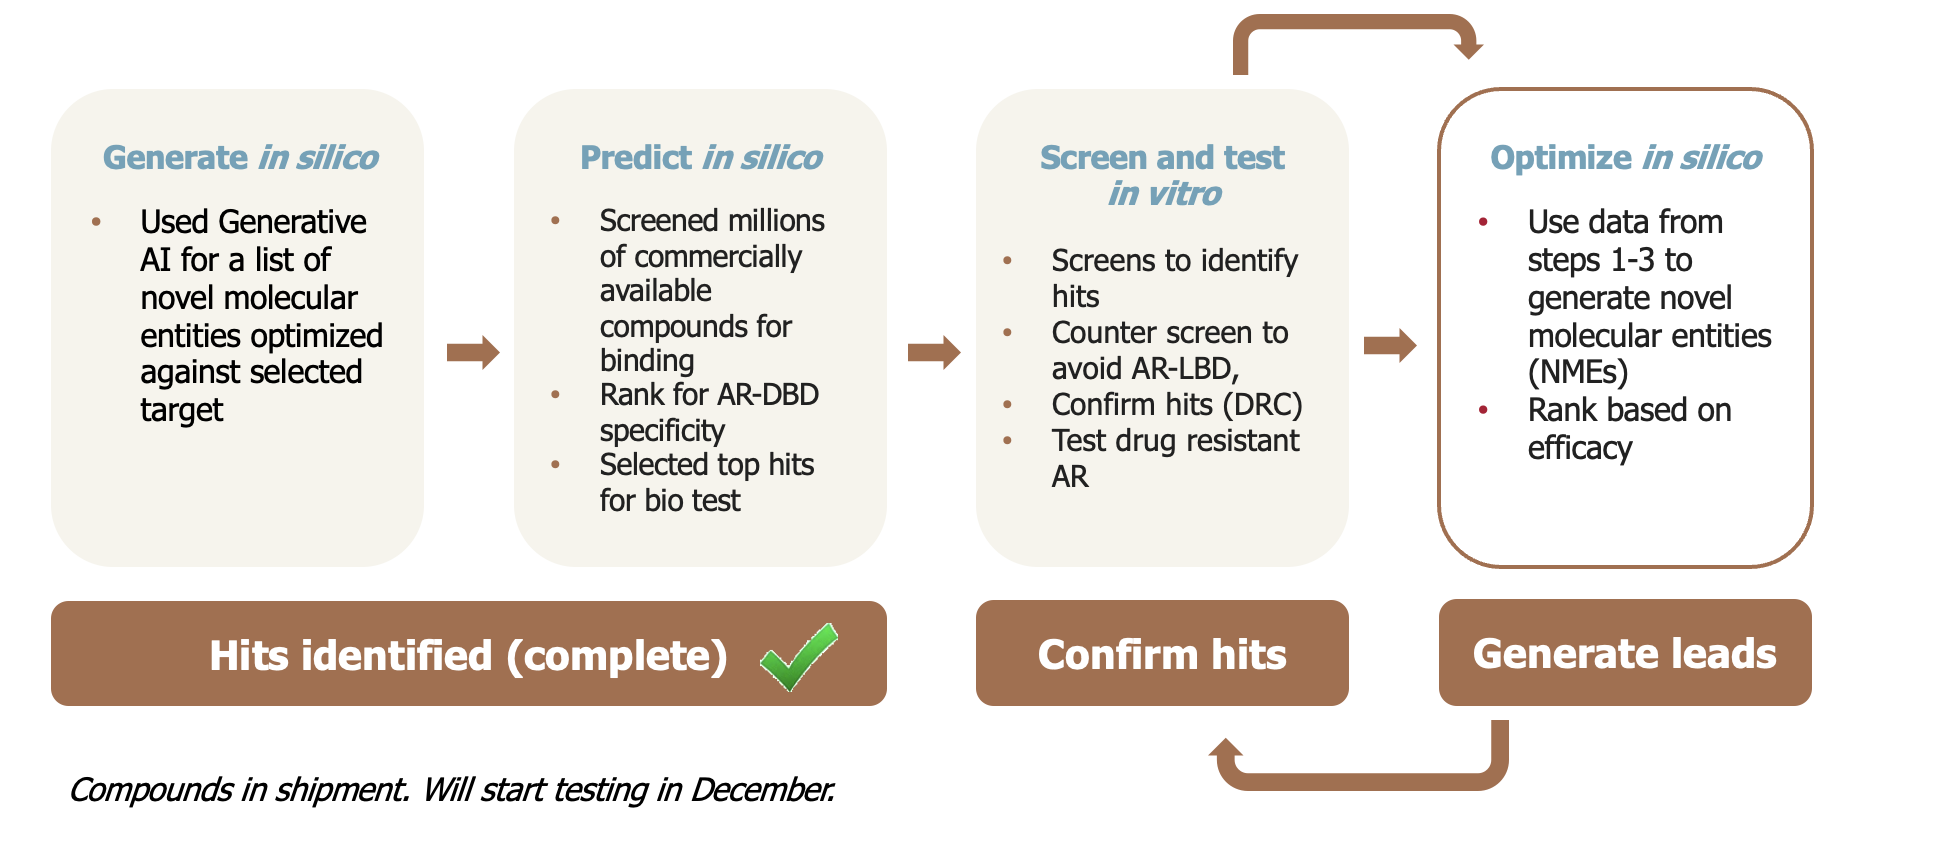
\includegraphics[width=1\linewidth]{../images/overall_workflow} \end{center}

\newpage

More specifically, this report analyzes assays from the target and
counter screen sections of the graphic below. Lab researchers led by
Mickey Huang used luciferase assays to screen 294 compounds generated by
SandboxAQ in silico. Then, they used this same assay to generate dose
response curves and conduct an AR Polar Binding Counter Screen.
Specificity assays are being optimized as of 4/24/2025.

\begin{center}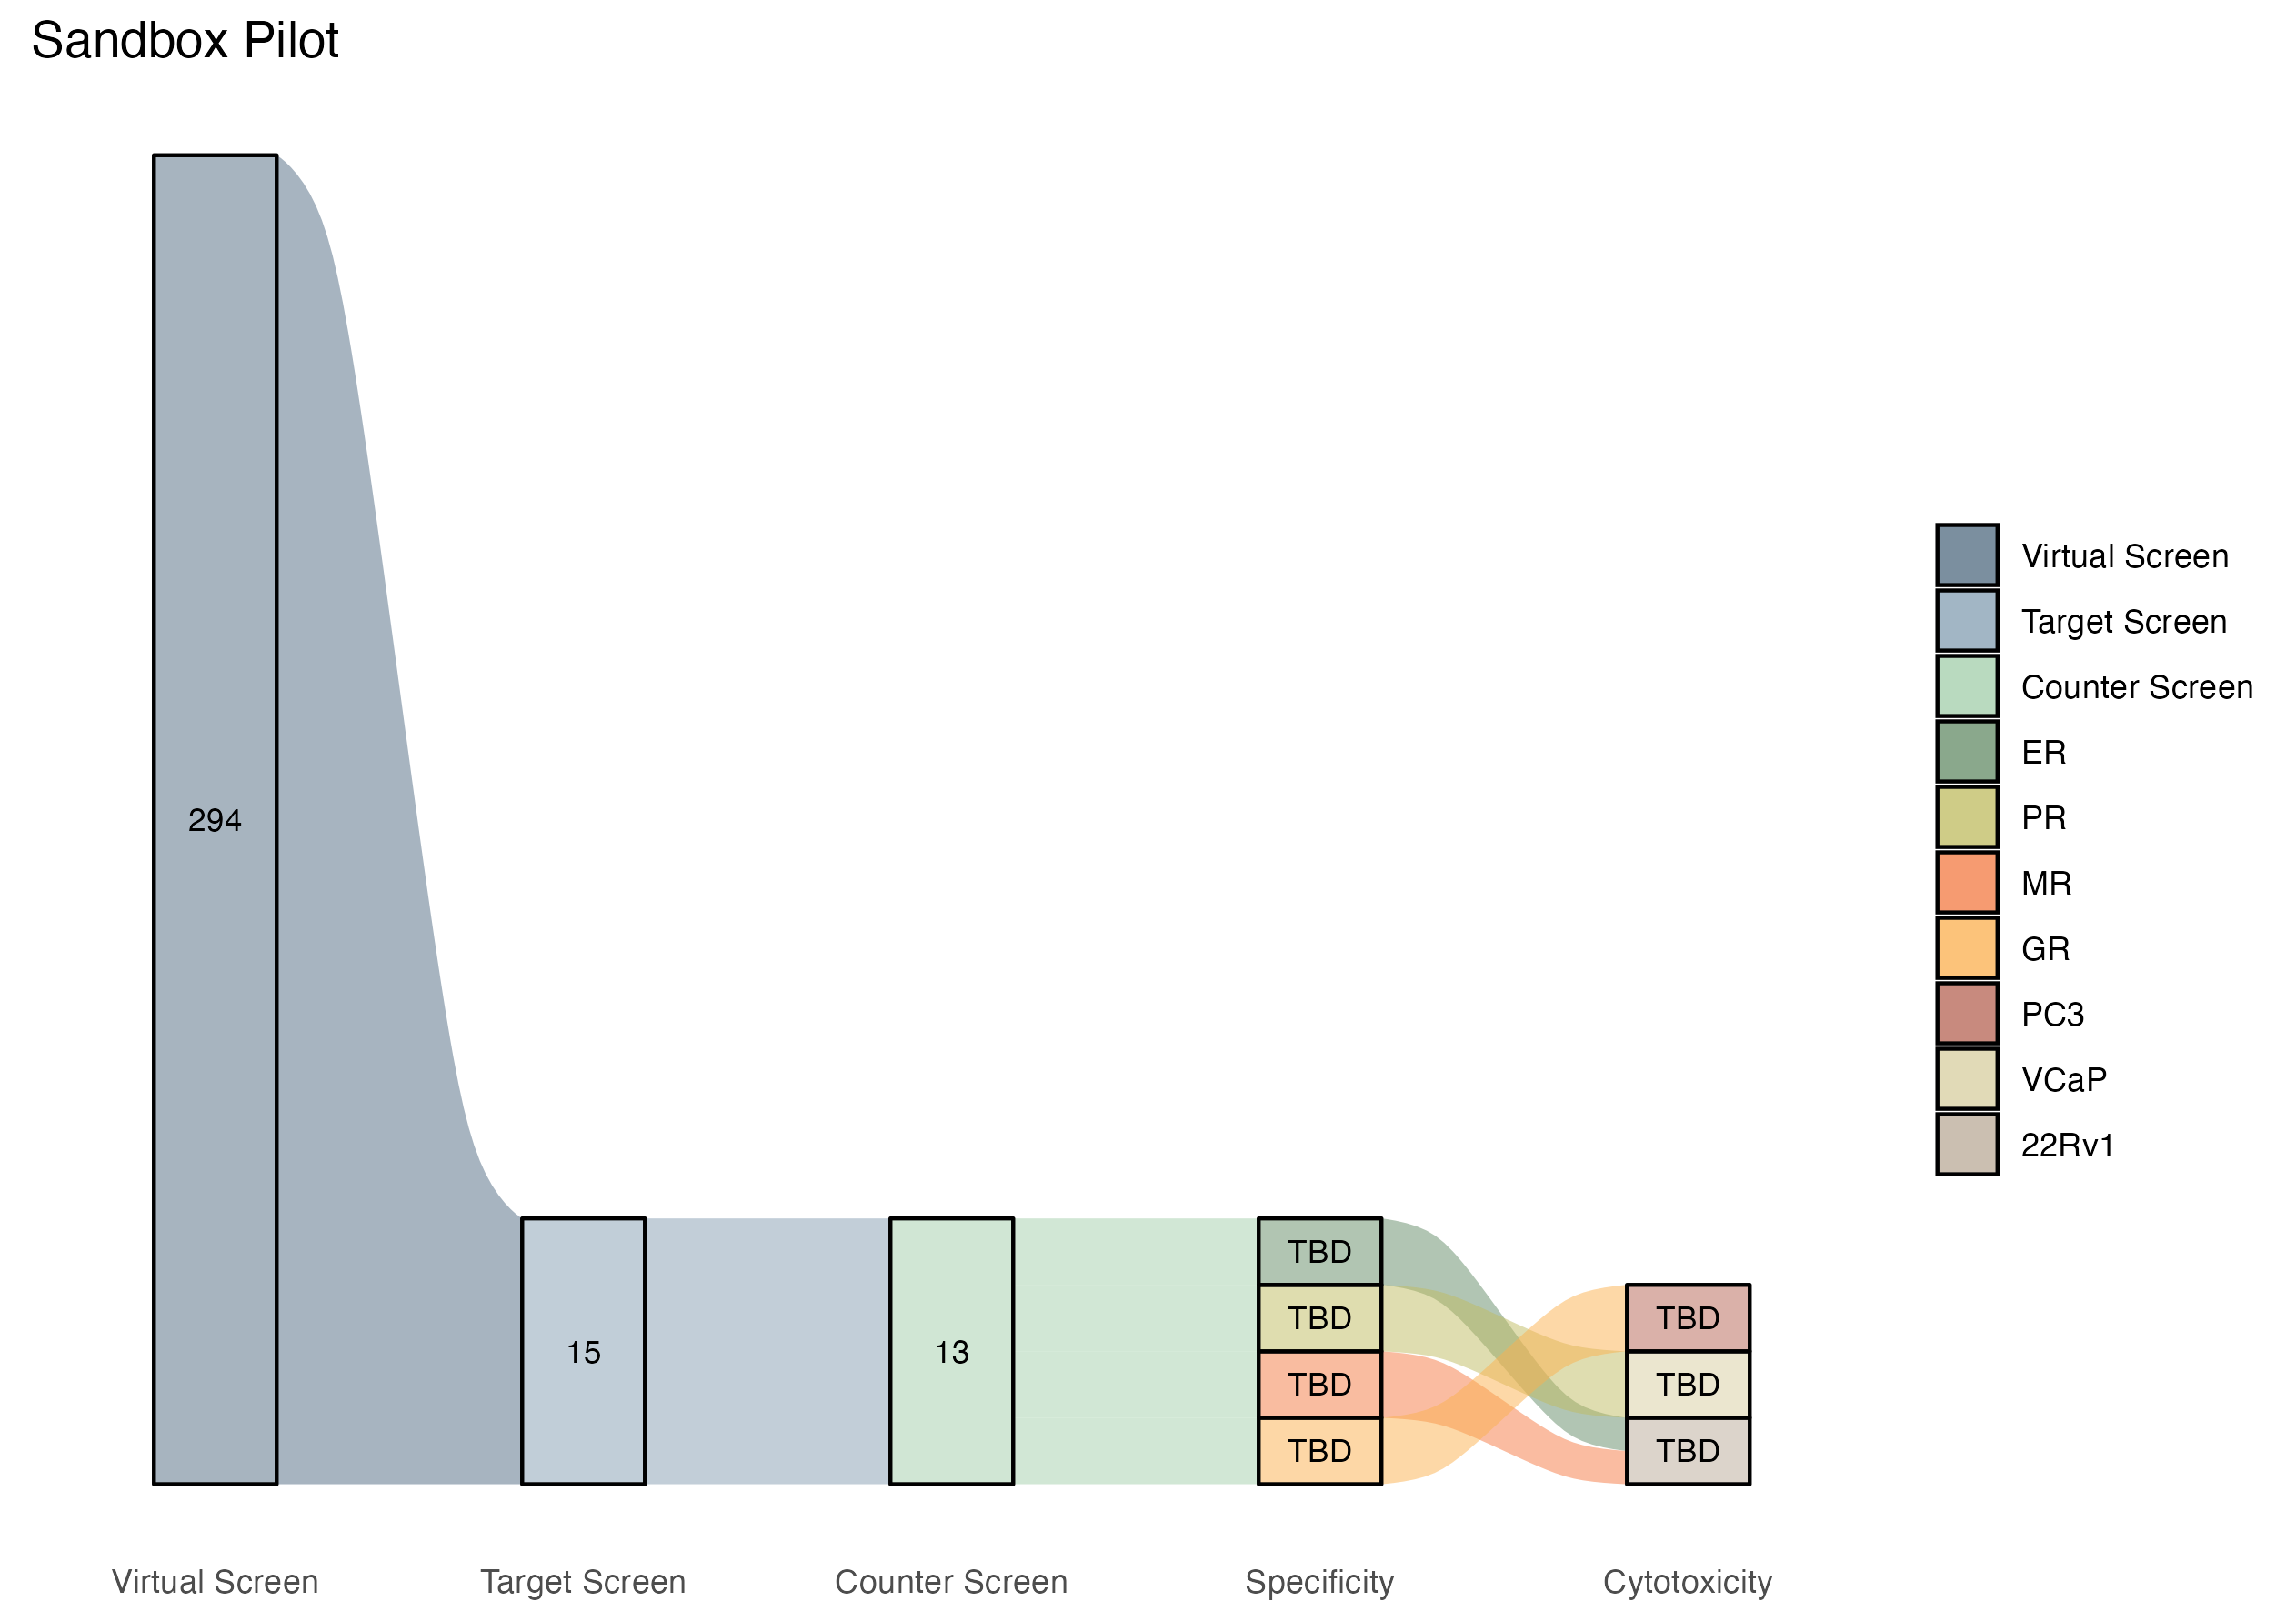
\includegraphics[width=1\linewidth]{../images/pilot_sankey} \end{center}

\newpage

\section{Overall Summary}\label{overall-summary}

\begin{itemize}
\tightlist
\item
  Initial Screen

  \begin{itemize}
  \tightlist
  \item
    In total, 68 had an average percent control lower than that of the
    100\% control - 3SD. This represents 24.29\% of the total number of
    compounds tested.
  \end{itemize}
\item
  Viability Dose Response

  \begin{itemize}
  \tightlist
  \item
    15 compounds were advanced to the next round of screening using
    interim criteria.
  \item
    16 compounds produced reliable relative and absolute EC50s (not
    extrapolated, RSE's below quantile outlier cutoff). In the table
    below, they are sorted by Absolute EC50.
  \end{itemize}
\end{itemize}

\begin{longtable}[]{@{}
  >{\raggedright\arraybackslash}p{(\columnwidth - 4\tabcolsep) * \real{0.6593}}
  >{\raggedright\arraybackslash}p{(\columnwidth - 4\tabcolsep) * \real{0.1868}}
  >{\raggedleft\arraybackslash}p{(\columnwidth - 4\tabcolsep) * \real{0.1538}}@{}}
\toprule\noalign{}
\begin{minipage}[b]{\linewidth}\raggedright
Experiment Name
\end{minipage} & \begin{minipage}[b]{\linewidth}\raggedright
Compound
\end{minipage} & \begin{minipage}[b]{\linewidth}\raggedleft
Absolute EC50
\end{minipage} \\
\midrule\noalign{}
\endhead
\bottomrule\noalign{}
\endlastfoot
New 20250128\_Luciferase\_Assay\_DRC\_priority2\_PC3\_K22\_ARE\_LUC &
MCULE-1287264115 & 31.64 \\
new 20250121\_Luciferase\_Assay\_DRC\_priority1\_PC3\_K22\_ARE\_LUC &
MCULE-1473251078 & 10.99 \\
New 20250128\_Luciferase\_Assay\_DRC\_priority2\_PC3\_K22\_ARE\_LUC &
MCULE-1862106206 & 14.75 \\
new 20250204\_Luciferase\_Assay\_DRC\_priority2\_PC3\_K22\_ARE-LUC &
MCULE-1862106206 & 10.18 \\
New 20250113\_Luciferase\_Assay\_DRC\_priority1\_PC3\_K22\_ARE\_LUC &
MCULE-2500215977 & 15.19 \\
New 20250128\_Luciferase\_Assay\_DRC\_priority2\_PC3\_K22\_ARE\_LUC &
MCULE-3983305475 & 17.33 \\
new 20250121\_Luciferase\_Assay\_DRC\_priority1\_PC3\_K22\_ARE\_LUC &
MCULE-4074783148 & 35.49 \\
new 20250121\_Luciferase\_Assay\_DRC\_priority1\_PC3\_K22\_ARE\_LUC &
MCULE-4701897276 & 27.67 \\
New 20250113\_Luciferase\_Assay\_DRC\_priority1\_PC3\_K22\_ARE\_LUC &
MCULE-4886311520 & 8.63 \\
new 20250121\_Luciferase\_Assay\_DRC\_priority1\_PC3\_K22\_ARE\_LUC &
MCULE-4886311520 & 7.87 \\
New 20250128\_Luciferase\_Assay\_DRC\_priority2\_PC3\_K22\_ARE\_LUC &
MCULE-5647507283 & 25.52 \\
new 20250204\_Luciferase\_Assay\_DRC\_priority2\_PC3\_K22\_ARE-LUC &
MCULE-5647507283 & 16.55 \\
new 20250121\_Luciferase\_Assay\_DRC\_priority1\_PC3\_K22\_ARE\_LUC &
MCULE-6507164368 & 30.90 \\
New 20250128\_Luciferase\_Assay\_DRC\_priority2\_PC3\_K22\_ARE\_LUC &
MCULE-9383018269 & 10.64 \\
new 20250204\_Luciferase\_Assay\_DRC\_priority2\_PC3\_K22\_ARE-LUC &
MCULE-9383018269 & 15.80 \\
New 20250128\_Luciferase\_Assay\_DRC\_priority2\_PC3\_K22\_ARE\_LUC &
MCULE-9598397280 & 21.13 \\
\end{longtable}

\begin{itemize}
\tightlist
\item
  Polar Binding Dose Response

  \begin{itemize}
  \tightlist
  \item
    15 compounds were included in the polar binding assay.
  \item
    6 compounds produced reliable relative and absolute EC50s (not
    extrapolated, RSE's below quantile outlier cutoff). In the table
    below, they are sorted by Absolute EC50.
  \end{itemize}
\end{itemize}

\begin{longtable}[]{@{}
  >{\raggedright\arraybackslash}p{(\columnwidth - 4\tabcolsep) * \real{0.6395}}
  >{\raggedright\arraybackslash}p{(\columnwidth - 4\tabcolsep) * \real{0.1977}}
  >{\raggedleft\arraybackslash}p{(\columnwidth - 4\tabcolsep) * \real{0.1628}}@{}}
\toprule\noalign{}
\begin{minipage}[b]{\linewidth}\raggedright
Experiment Name
\end{minipage} & \begin{minipage}[b]{\linewidth}\raggedright
Compound
\end{minipage} & \begin{minipage}[b]{\linewidth}\raggedleft
Absolute EC50
\end{minipage} \\
\midrule\noalign{}
\endhead
\bottomrule\noalign{}
\endlastfoot
20250326\_Polar Screen AR competitor assay Rep 2\_680426 &
MCULE-1473251078 & 19.85 \\
20250224\_PolarScreen\_Priority\_Compounds\_646129 & MCULE-1473251078 &
52.90 \\
20250326\_Polar Screen AR competitor assay Rep 2\_680426 &
MCULE-3983305476 & 73.22 \\
20250326\_Polar Screen AR competitor assay Rep 2\_680426 &
MCULE-4701897276 & 3.27 \\
20250224\_PolarScreen\_Priority\_Compounds\_646129 & MCULE-4701897276 &
15.90 \\
20250326\_Polar Screen AR competitor assay Rep 2\_680426 &
MCULE-9598397280 & 61.90 \\
\end{longtable}

\newpage

\section{Quality Control}\label{quality-control}

\subsection{Overall Summary}\label{overall-summary-1}

question: should we be calling these ``cutoffs''?

We collect these assay quality control statistics:

\begin{itemize}
\tightlist
\item
  Z'Factor

  \begin{itemize}
  \tightlist
  \item
    measures separation between high and low controls
  \item
    cutoff: \textless{} 0
  \end{itemize}
\item
  Average Intra-Assay \%CV, or Average\%CV

  \begin{itemize}
  \tightlist
  \item
    measures overall assay variation
  \item
    cutoff: \textgreater{} quantile outlier bound
  \end{itemize}
\end{itemize}

\begin{longtable}[]{@{}
  >{\raggedright\arraybackslash}p{(\columnwidth - 12\tabcolsep) * \real{0.0667}}
  >{\raggedright\arraybackslash}p{(\columnwidth - 12\tabcolsep) * \real{0.0429}}
  >{\raggedright\arraybackslash}p{(\columnwidth - 12\tabcolsep) * \real{0.2048}}
  >{\raggedright\arraybackslash}p{(\columnwidth - 12\tabcolsep) * \real{0.0952}}
  >{\raggedright\arraybackslash}p{(\columnwidth - 12\tabcolsep) * \real{0.0952}}
  >{\raggedright\arraybackslash}p{(\columnwidth - 12\tabcolsep) * \real{0.2476}}
  >{\raggedright\arraybackslash}p{(\columnwidth - 12\tabcolsep) * \real{0.2476}}@{}}
\toprule\noalign{}
\begin{minipage}[b]{\linewidth}\raggedright
Experiment ID
\end{minipage} & \begin{minipage}[b]{\linewidth}\raggedright
Plate ID
\end{minipage} & \begin{minipage}[b]{\linewidth}\raggedright
Experiment Type
\end{minipage} & \begin{minipage}[b]{\linewidth}\raggedright
Assay Type
\end{minipage} & \begin{minipage}[b]{\linewidth}\raggedright
Start Date
\end{minipage} & \begin{minipage}[b]{\linewidth}\raggedright
Plate Z'Factor
\end{minipage} & \begin{minipage}[b]{\linewidth}\raggedright
Summary Percent CV
\end{minipage} \\
\midrule\noalign{}
\endhead
\bottomrule\noalign{}
\endlastfoot
679577 & 1479 & Luciferase Assay & Screen & 2024-12-16 00:00:00 &
\cellcolor[HTML]{A96D4B}{\textcolor{white}{-0.146}} &
\cellcolor{white}{\textcolor{black}{12.61}} \\
679577 & 1480 & Luciferase Assay & Screen & 2024-12-16 00:00:00 &
\cellcolor{white}{\textcolor{black}{0.594}} &
\cellcolor{white}{\textcolor{black}{12.61}} \\
679577 & 1481 & Luciferase Assay & Screen & 2024-12-16 00:00:00 &
\cellcolor{white}{\textcolor{black}{0.501}} &
\cellcolor{white}{\textcolor{black}{12.61}} \\
679768 & 1482 & Luciferase Assay & Screen & 2025-03-26 10:06:39 &
\cellcolor{white}{\textcolor{black}{0.697}} &
\cellcolor{white}{\textcolor{black}{12.964}} \\
679768 & 1483 & Luciferase Assay & Screen & 2025-03-26 10:06:39 &
\cellcolor{white}{\textcolor{black}{0.65}} &
\cellcolor{white}{\textcolor{black}{12.964}} \\
679768 & 1484 & Luciferase Assay & Screen & 2025-03-26 10:06:39 &
\cellcolor{white}{\textcolor{black}{0.776}} &
\cellcolor{white}{\textcolor{black}{12.964}} \\
679915 & 1485 & Luciferase Assay & Screen & 2024-12-18 00:00:00 &
\cellcolor{white}{\textcolor{black}{0.622}} &
\cellcolor{white}{\textcolor{black}{17.649}} \\
679915 & 1486 & Luciferase Assay & Screen & 2024-12-18 00:00:00 &
\cellcolor{white}{\textcolor{black}{0.676}} &
\cellcolor{white}{\textcolor{black}{17.649}} \\
679915 & 1487 & Luciferase Assay & Screen & 2024-12-18 00:00:00 &
\cellcolor{white}{\textcolor{black}{0.665}} &
\cellcolor{white}{\textcolor{black}{17.649}} \\
680021 & 1495 & Luciferase Assay & Screen & 2025-01-06 00:00:00 &
\cellcolor{white}{\textcolor{black}{0.19}} &
\cellcolor[HTML]{A96D4B}{\textcolor{white}{69.297}} \\
680021 & 1496 & Luciferase Assay & Screen & 2025-01-06 00:00:00 &
\cellcolor[HTML]{A96D4B}{\textcolor{white}{-0.102}} &
\cellcolor[HTML]{A96D4B}{\textcolor{white}{69.297}} \\
680021 & 1497 & Luciferase Assay & Screen & 2025-01-06 00:00:00 &
\cellcolor[HTML]{A96D4B}{\textcolor{white}{-0.161}} &
\cellcolor[HTML]{A96D4B}{\textcolor{white}{69.297}} \\
680122 & 1498 & Luciferase Assay & Screen & 2025-03-26 11:46:32 &
\cellcolor{white}{\textcolor{black}{0.711}} &
\cellcolor{white}{\textcolor{black}{24.524}} \\
680122 & 1499 & Luciferase Assay & Screen & 2025-03-26 11:46:32 &
\cellcolor{white}{\textcolor{black}{0.89}} &
\cellcolor{white}{\textcolor{black}{24.524}} \\
680122 & 1500 & Luciferase Assay & Screen & 2025-03-26 11:46:32 &
\cellcolor{white}{\textcolor{black}{0.834}} &
\cellcolor{white}{\textcolor{black}{24.524}} \\
686250 & 1501 & Dose Response Curve (DRC),Luciferase Assay & Dose
Response Curve & 2025-01-03 00:00:00 &
\cellcolor{white}{\textcolor{black}{0.707}} &
\cellcolor{white}{\textcolor{black}{5.142}} \\
686250 & 1502 & Dose Response Curve (DRC),Luciferase Assay & Dose
Response Curve & 2025-01-03 00:00:00 &
\cellcolor{white}{\textcolor{black}{0.892}} &
\cellcolor{white}{\textcolor{black}{5.6}} \\
686250 & 1503 & Dose Response Curve (DRC),Luciferase Assay & Dose
Response Curve & 2025-01-03 00:00:00 &
\cellcolor{white}{\textcolor{black}{0.679}} &
\cellcolor{white}{\textcolor{black}{6.129}} \\
686250 & 1504 & Dose Response Curve (DRC),Luciferase Assay & Dose
Response Curve & 2025-01-03 00:00:00 &
\cellcolor{white}{\textcolor{black}{0.747}} &
\cellcolor{white}{\textcolor{black}{8.264}} \\
686372 & 1505 & Dose Response Curve (DRC),Luciferase Assay & Dose
Response Curve & 2025-01-21 00:00:00 &
\cellcolor{white}{\textcolor{black}{0.554}} &
\cellcolor{white}{\textcolor{black}{12.39}} \\
686372 & 1506 & Dose Response Curve (DRC),Luciferase Assay & Dose
Response Curve & 2025-01-21 00:00:00 &
\cellcolor{white}{\textcolor{black}{0.591}} &
\cellcolor{white}{\textcolor{black}{14.649}} \\
686372 & 1507 & Dose Response Curve (DRC),Luciferase Assay & Dose
Response Curve & 2025-01-21 00:00:00 &
\cellcolor{white}{\textcolor{black}{0.617}} &
\cellcolor{white}{\textcolor{black}{9.831}} \\
686372 & 1508 & Dose Response Curve (DRC),Luciferase Assay & Dose
Response Curve & 2025-01-21 00:00:00 &
\cellcolor{white}{\textcolor{black}{0.616}} &
\cellcolor{white}{\textcolor{black}{10.336}} \\
686503 & 1509 & Dose Response Curve (DRC),Luciferase Assay & Dose
Response Curve & 2025-01-28 00:00:00 &
\cellcolor{white}{\textcolor{black}{0.805}} &
\cellcolor{white}{\textcolor{black}{12.378}} \\
686503 & 1510 & Dose Response Curve (DRC),Luciferase Assay & Dose
Response Curve & 2025-01-28 00:00:00 &
\cellcolor{white}{\textcolor{black}{0.71}} &
\cellcolor{white}{\textcolor{black}{7.052}} \\
686503 & 1511 & Dose Response Curve (DRC),Luciferase Assay & Dose
Response Curve & 2025-01-28 00:00:00 &
\cellcolor{white}{\textcolor{black}{0.822}} &
\cellcolor{white}{\textcolor{black}{14.717}} \\
686503 & 1512 & Dose Response Curve (DRC),Luciferase Assay & Dose
Response Curve & 2025-01-28 00:00:00 &
\cellcolor{white}{\textcolor{black}{0.806}} &
\cellcolor{white}{\textcolor{black}{6.305}} \\
686609 & 1513 & Dose Response Curve (DRC),Luciferase Assay & Dose
Response Curve & 2025-02-04 00:00:00 &
\cellcolor{white}{\textcolor{black}{0.877}} &
\cellcolor{white}{\textcolor{black}{12.53}} \\
686609 & 1514 & Dose Response Curve (DRC),Luciferase Assay & Dose
Response Curve & 2025-02-04 00:00:00 &
\cellcolor{white}{\textcolor{black}{0.737}} &
\cellcolor{white}{\textcolor{black}{10.066}} \\
686609 & 1515 & Dose Response Curve (DRC),Luciferase Assay & Dose
Response Curve & 2025-02-04 00:00:00 &
\cellcolor{white}{\textcolor{black}{0.872}} &
\cellcolor{white}{\textcolor{black}{7.3}} \\
686609 & 1516 & Dose Response Curve (DRC),Luciferase Assay & Dose
Response Curve & 2025-02-04 00:00:00 &
\cellcolor{white}{\textcolor{black}{0.866}} &
\cellcolor{white}{\textcolor{black}{6.112}} \\
680426 & 1521 & AR Binding & Polar Binding & 2025-03-26 15:06:16 &
\cellcolor{white}{\textcolor{black}{0.114}} &
\cellcolor{white}{\textcolor{black}{2.947}} \\
689281 & 1520 & AR Binding & Polar Binding & 2025-04-10 10:14:36 &
\cellcolor{white}{\textcolor{black}{0.522}} &
\cellcolor{white}{\textcolor{black}{2.781}} \\
\end{longtable}

\newpage

\subsection{Z'Factor}\label{zfactor}

This QC statistic measures the separation band between high and low
controls.

\begin{center}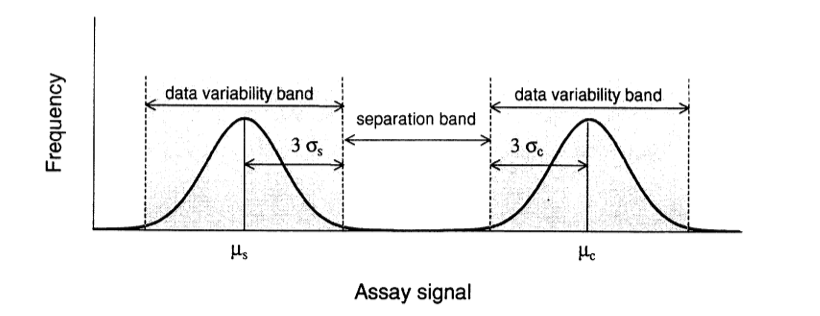
\includegraphics[width=1\linewidth]{../images/zfactor_explainer} \end{center}

Z'Factor is calculated with the following formula:

\[
\text{Z'Factor} = 1 - \frac{3*(\sigma_{c^{+}} - \sigma_{c^{-}})}{|\mu_{c^{+}} - \mu_{c^{-}}|}
\]

A Z'Factor above 0 is considered sufficient at EMI.

\href{https://pubmed.ncbi.nlm.nih.gov/10838414/}{Further reading.}

\newpage

\begin{center}\includegraphics[width=0.8\linewidth]{round1_init-screen-thru-counter-screen_files/figure-latex/qcbox-1} \end{center}

The above plot shows Z'factors calculated for each plate. There are 3
plates with Z'factors less than 0. These plates are numbered: 1479,
1496, 1497.

\begin{center}\includegraphics{round1_init-screen-thru-counter-screen_files/figure-latex/zprime-1} \end{center}

These plots show that high variability in 100\% control conditions are
likely the cause for the low Z'Factors in this plate.

Also of note: many molecules generated by the SandboxAQ algorithm and in
silico screen produce RLU higher than the 100\% control condition.

\newpage

For further examination, below are plate heat maps for each plate with a
Z'Factor less than 0.

\paragraph{Platemap for Plate 1479 , Experiment
679577}\label{platemap-for-plate-1479-experiment-679577}

\begin{center}\includegraphics{round1_init-screen-thru-counter-screen_files/figure-latex/platemaps-1} \end{center}

\newpage

\paragraph{Platemap for Plate 1496 , Experiment
680021}\label{platemap-for-plate-1496-experiment-680021}

\begin{center}\includegraphics{round1_init-screen-thru-counter-screen_files/figure-latex/platemaps-2} \end{center}

\newpage

\paragraph{Platemap for Plate 1497 , Experiment
680021}\label{platemap-for-plate-1497-experiment-680021}

\begin{center}\includegraphics{round1_init-screen-thru-counter-screen_files/figure-latex/platemaps-3} \end{center}

\newpage[[1]

{]} NULL

{[}{[}2{]}{]} NULL

{[}{[}3{]}{]} NULL

\newpage

\subsection{Average Intra-Assay \%CV}\label{average-intra-assay-cv}

Average Intra-Assay \%CV is measure on a \([0, +\inf]\) scale. A higher
Average\%CV indicates a higher level of variability in the assay. It is
calculated by taking the mean of all Intra-Assay \%CVs over all
conditions of an assay. Intra-Assay \%CV is calculated for each
condition in an assay by dividing the standard deviation of its signals
by the mean of its signals.

\href{https://toptipbio.com/calculate-coefficient-variation-cv/}{Further
reading.}

Unlike Z'Factor, Average Intra-Assay \%CV does not have a built-in
cutoff. For this project, we will collect Average\%CV's for all assays
and calculate their quantile outlier bounds. This will serve as a
cutoff.

\begin{longtable}[]{@{}lr@{}}
\toprule\noalign{}
Assay Type & Summary \%CV Cutoff \\
\midrule\noalign{}
\endhead
\bottomrule\noalign{}
\endlastfoot
Screen & 41.864911 \\
Dose Response Curve & 21.561305 \\
Polar Binding & 3.029843 \\
\end{longtable}

\begin{center}\includegraphics[width=0.7\linewidth]{round1_init-screen-thru-counter-screen_files/figure-latex/cvs-1} \end{center}

\begin{center}\includegraphics{round1_init-screen-thru-counter-screen_files/figure-latex/cv_outliers-1} \end{center}

Experiment 680021 appears to have high variability within all compounds.
Especially of note is the apparently high variation in the condition
R1881, which served as our 100\% control. Two of the plates (in this
project, screens have technical replicates across plates) in this
experiment, specifially 1496 and 1497, were also flagged for Z'Factors
lower than 0.

\newpage

\section{Initial Screen}\label{initial-screen}

The purpose of the initial screen was to designate ``hit compounds,''
which would then move to the next phase of testing.

This was a viability assay, meaning that low RLU indicates cell death.

In this project, screens have technical replicates across plates.

In the following plots, horizontal lines represent hit designation
cutoffs at 3-9 standard deviations away from the mean of the 100\%
control. Lower lines serve as stricter cutoffs for designating hits.

Z'Factor is calculated relative to 0\% control condition.

In total, 68 had an average percent control lower than that of the 100\%
control - 3SD. This represents 24.29\% of the total number of compounds
tested.

\subsection{679577 All Compounds}\label{all-compounds}

\begin{center}\includegraphics{round1_init-screen-thru-counter-screen_files/figure-latex/initial_screen_plots-1} \end{center}

\newpage

\subsection{679915 All Compounds}\label{all-compounds-1}

\begin{center}\includegraphics{round1_init-screen-thru-counter-screen_files/figure-latex/initial_screen_plots-2} \end{center}

\newpage

\subsection{680021 All Compounds}\label{all-compounds-2}

\begin{center}\includegraphics{round1_init-screen-thru-counter-screen_files/figure-latex/initial_screen_plots-3} \end{center}

\newpage

\subsection{679768 All Compounds}\label{all-compounds-3}

\begin{center}\includegraphics{round1_init-screen-thru-counter-screen_files/figure-latex/initial_screen_plots-4} \end{center}

\newpage

\subsection{680122 All Compounds}\label{all-compounds-4}

\begin{center}\includegraphics{round1_init-screen-thru-counter-screen_files/figure-latex/initial_screen_plots-5} \end{center}

\newpage
\newpage

see fold change plot

\begin{center}\includegraphics{round1_init-screen-thru-counter-screen_files/figure-latex/fcplot-1} \end{center}

\subsection{Designated Hits}\label{designated-hits}

how many 9sd hits for each experiment? and see z'factors for each

\begin{center}\includegraphics{round1_init-screen-thru-counter-screen_files/figure-latex/hitplots-1} \end{center}

\begin{longtable}[]{@{}
  >{\raggedright\arraybackslash}p{(\columnwidth - 12\tabcolsep) * \real{0.1750}}
  >{\raggedright\arraybackslash}p{(\columnwidth - 12\tabcolsep) * \real{0.2500}}
  >{\raggedleft\arraybackslash}p{(\columnwidth - 12\tabcolsep) * \real{0.0875}}
  >{\raggedleft\arraybackslash}p{(\columnwidth - 12\tabcolsep) * \real{0.1375}}
  >{\raggedright\arraybackslash}p{(\columnwidth - 12\tabcolsep) * \real{0.1375}}
  >{\raggedleft\arraybackslash}p{(\columnwidth - 12\tabcolsep) * \real{0.1125}}
  >{\raggedright\arraybackslash}p{(\columnwidth - 12\tabcolsep) * \real{0.1000}}@{}}
\toprule\noalign{}
\begin{minipage}[b]{\linewidth}\raggedright
experiment\_id
\end{minipage} & \begin{minipage}[b]{\linewidth}\raggedright
start\_date
\end{minipage} & \begin{minipage}[b]{\linewidth}\raggedleft
exp\_cv
\end{minipage} & \begin{minipage}[b]{\linewidth}\raggedleft
exp\_zprime
\end{minipage} & \begin{minipage}[b]{\linewidth}\raggedright
coi\_lab
\end{minipage} & \begin{minipage}[b]{\linewidth}\raggedleft
coi\_dose
\end{minipage} & \begin{minipage}[b]{\linewidth}\raggedright
scr\_hit
\end{minipage} \\
\midrule\noalign{}
\endhead
\bottomrule\noalign{}
\endlastfoot
679915 & 2024-12-18 00:00:00 & 17.649 & 0.665 & 1473251078 & 30 & 9SD
hit \\
679768 & 2025-03-26 10:06:39 & 12.964 & 0.622 & 1862106206 & 30 & 9SD
hit \\
679768 & 2025-03-26 10:06:39 & 12.964 & 0.622 & 5647507283 & 30 & 9SD
hit \\
680122 & 2025-03-26 11:46:32 & 24.524 & 0.518 & 1287264115 & 30 & 9SD
hit \\
680122 & 2025-03-26 11:46:32 & 24.524 & 0.518 & 2500215977 & 30 & 9SD
hit \\
680122 & 2025-03-26 11:46:32 & 24.524 & 0.518 & 4074783148 & 30 & 9SD
hit \\
680122 & 2025-03-26 11:46:32 & 24.524 & 0.518 & 4886311520 & 30 & 9SD
hit \\
680122 & 2025-03-26 11:46:32 & 24.524 & 0.518 & 7049591067 & 30 & 9SD
hit \\
680122 & 2025-03-26 11:46:32 & 24.524 & 0.518 & 8006451741 & 30 & 9SD
hit \\
680122 & 2025-03-26 11:46:32 & 24.524 & 0.518 & 9383018269 & 30 & 9SD
hit \\
\end{longtable}

\newpage

\section{Dose Response}\label{dose-response}

The purpose of this assay was to further investigate our hits by
modelling their dose responses.

This was a viability assay, meaning that low RLU indicates cell death.

Response is normalized to control using this formula:

\[
\frac{\text{signal} - mean(\text{0% control signal})}{mean(\text{100% control signal}) - mean(\text{0% control signal})}
\]

The following table includes all compounds that achieved 50\% (absolute
and relative) inhibition without extrapolating. Compounds with outlier
RSE's are excluded.

\begin{longtable}[]{@{}
  >{\raggedright\arraybackslash}p{(\columnwidth - 8\tabcolsep) * \real{0.1284}}
  >{\raggedright\arraybackslash}p{(\columnwidth - 8\tabcolsep) * \real{0.5505}}
  >{\raggedright\arraybackslash}p{(\columnwidth - 8\tabcolsep) * \real{0.1560}}
  >{\raggedleft\arraybackslash}p{(\columnwidth - 8\tabcolsep) * \real{0.0826}}
  >{\raggedleft\arraybackslash}p{(\columnwidth - 8\tabcolsep) * \real{0.0826}}@{}}
\toprule\noalign{}
\begin{minipage}[b]{\linewidth}\raggedright
experiment\_id
\end{minipage} & \begin{minipage}[b]{\linewidth}\raggedright
experiment\_name
\end{minipage} & \begin{minipage}[b]{\linewidth}\raggedright
coi
\end{minipage} & \begin{minipage}[b]{\linewidth}\raggedleft
abs\_ec50
\end{minipage} & \begin{minipage}[b]{\linewidth}\raggedleft
rel\_ec50
\end{minipage} \\
\midrule\noalign{}
\endhead
\bottomrule\noalign{}
\endlastfoot
686503 & New
20250128\_Luciferase\_Assay\_DRC\_priority2\_PC3\_K22\_ARE\_LUC &
MCULE-1287264115 & 31.639 & 30.626 \\
686372 & new
20250121\_Luciferase\_Assay\_DRC\_priority1\_PC3\_K22\_ARE\_LUC &
MCULE-1473251078 & 10.993 & 25.179 \\
686503 & New
20250128\_Luciferase\_Assay\_DRC\_priority2\_PC3\_K22\_ARE\_LUC &
MCULE-1862106206 & 14.749 & 15.424 \\
686609 & new
20250204\_Luciferase\_Assay\_DRC\_priority2\_PC3\_K22\_ARE-LUC &
MCULE-1862106206 & 10.181 & 13.541 \\
686250 & New
20250113\_Luciferase\_Assay\_DRC\_priority1\_PC3\_K22\_ARE\_LUC &
MCULE-2500215977 & 15.194 & 13.818 \\
686503 & New
20250128\_Luciferase\_Assay\_DRC\_priority2\_PC3\_K22\_ARE\_LUC &
MCULE-3983305475 & 17.332 & 20.629 \\
686372 & new
20250121\_Luciferase\_Assay\_DRC\_priority1\_PC3\_K22\_ARE\_LUC &
MCULE-4074783148 & 35.486 & 36.468 \\
686372 & new
20250121\_Luciferase\_Assay\_DRC\_priority1\_PC3\_K22\_ARE\_LUC &
MCULE-4701897276 & 27.672 & 26.852 \\
686250 & New
20250113\_Luciferase\_Assay\_DRC\_priority1\_PC3\_K22\_ARE\_LUC &
MCULE-4886311520 & 8.630 & 9.187 \\
686372 & new
20250121\_Luciferase\_Assay\_DRC\_priority1\_PC3\_K22\_ARE\_LUC &
MCULE-4886311520 & 7.867 & 7.646 \\
686503 & New
20250128\_Luciferase\_Assay\_DRC\_priority2\_PC3\_K22\_ARE\_LUC &
MCULE-5647507283 & 25.517 & 12.032 \\
686609 & new
20250204\_Luciferase\_Assay\_DRC\_priority2\_PC3\_K22\_ARE-LUC &
MCULE-5647507283 & 16.550 & 40.689 \\
686372 & new
20250121\_Luciferase\_Assay\_DRC\_priority1\_PC3\_K22\_ARE\_LUC &
MCULE-6507164368 & 30.898 & 30.337 \\
686503 & New
20250128\_Luciferase\_Assay\_DRC\_priority2\_PC3\_K22\_ARE\_LUC &
MCULE-9383018269 & 10.641 & 9.611 \\
686609 & new
20250204\_Luciferase\_Assay\_DRC\_priority2\_PC3\_K22\_ARE-LUC &
MCULE-9383018269 & 15.799 & 13.002 \\
686503 & New
20250128\_Luciferase\_Assay\_DRC\_priority2\_PC3\_K22\_ARE\_LUC &
MCULE-9598397280 & 21.132 & 19.315 \\
\end{longtable}

16 molecules of the 30 tested (53.3333333) produced quality EC50s.

\newpage

\subsection{MCULE-1287264115}\label{mcule-1287264115}

MCULE-1287264115 Raw Plot

\begin{center}\includegraphics{round1_init-screen-thru-counter-screen_files/figure-latex/drcs-1} \end{center}

\begin{longtable}[]{@{}
  >{\raggedright\arraybackslash}p{(\columnwidth - 18\tabcolsep) * \real{0.1007}}
  >{\raggedright\arraybackslash}p{(\columnwidth - 18\tabcolsep) * \real{0.1439}}
  >{\raggedright\arraybackslash}p{(\columnwidth - 18\tabcolsep) * \real{0.0647}}
  >{\raggedleft\arraybackslash}p{(\columnwidth - 18\tabcolsep) * \real{0.0719}}
  >{\raggedleft\arraybackslash}p{(\columnwidth - 18\tabcolsep) * \real{0.1079}}
  >{\raggedleft\arraybackslash}p{(\columnwidth - 18\tabcolsep) * \real{0.1079}}
  >{\raggedleft\arraybackslash}p{(\columnwidth - 18\tabcolsep) * \real{0.0935}}
  >{\raggedleft\arraybackslash}p{(\columnwidth - 18\tabcolsep) * \real{0.1007}}
  >{\raggedleft\arraybackslash}p{(\columnwidth - 18\tabcolsep) * \real{0.0863}}
  >{\raggedleft\arraybackslash}p{(\columnwidth - 18\tabcolsep) * \real{0.1223}}@{}}
\toprule\noalign{}
\begin{minipage}[b]{\linewidth}\raggedright
Experiment ID
\end{minipage} & \begin{minipage}[b]{\linewidth}\raggedright
Start Date
\end{minipage} & \begin{minipage}[b]{\linewidth}\raggedright
Plate ID
\end{minipage} & \begin{minipage}[b]{\linewidth}\raggedleft
Plate \%CV
\end{minipage} & \begin{minipage}[b]{\linewidth}\raggedleft
Plate Z'Factor
\end{minipage} & \begin{minipage}[b]{\linewidth}\raggedleft
Mean R1881 RLU
\end{minipage} & \begin{minipage}[b]{\linewidth}\raggedleft
SD R1881 RLU
\end{minipage} & \begin{minipage}[b]{\linewidth}\raggedleft
Mean DMSO RLU
\end{minipage} & \begin{minipage}[b]{\linewidth}\raggedleft
SD DMSO RLU
\end{minipage} & \begin{minipage}[b]{\linewidth}\raggedleft
Plate \%CV Cutoff
\end{minipage} \\
\midrule\noalign{}
\endhead
\bottomrule\noalign{}
\endlastfoot
686503 & 2025-01-28 00:00:00 & 1512 & 15.285 & 0.965 & 505928.8 &
31028.74 & 12649.67 & 803.262 & 21.561 \\
686609 & 2025-02-04 00:00:00 & 1516 & 14.760 & 0.919 & 716364.7 &
30393.05 & 16944.67 & 872.006 & 21.561 \\
\end{longtable}

\newpage

MCULE-1287264115 Normalized Plot

\begin{center}\includegraphics{round1_init-screen-thru-counter-screen_files/figure-latex/drcs-2} \end{center}

\begin{longtable}[]{@{}
  >{\raggedright\arraybackslash}p{(\columnwidth - 18\tabcolsep) * \real{0.0733}}
  >{\raggedright\arraybackslash}p{(\columnwidth - 18\tabcolsep) * \real{0.0400}}
  >{\raggedleft\arraybackslash}p{(\columnwidth - 18\tabcolsep) * \real{0.0933}}
  >{\raggedright\arraybackslash}p{(\columnwidth - 18\tabcolsep) * \real{0.1133}}
  >{\raggedleft\arraybackslash}p{(\columnwidth - 18\tabcolsep) * \real{0.0933}}
  >{\raggedright\arraybackslash}p{(\columnwidth - 18\tabcolsep) * \real{0.1133}}
  >{\raggedleft\arraybackslash}p{(\columnwidth - 18\tabcolsep) * \real{0.0467}}
  >{\raggedleft\arraybackslash}p{(\columnwidth - 18\tabcolsep) * \real{0.0733}}
  >{\raggedright\arraybackslash}p{(\columnwidth - 18\tabcolsep) * \real{0.1733}}
  >{\raggedright\arraybackslash}p{(\columnwidth - 18\tabcolsep) * \real{0.1800}}@{}}
\toprule\noalign{}
\begin{minipage}[b]{\linewidth}\raggedright
Experiment
\end{minipage} & \begin{minipage}[b]{\linewidth}\raggedright
Plate
\end{minipage} & \begin{minipage}[b]{\linewidth}\raggedleft
Absolute EC50
\end{minipage} & \begin{minipage}[b]{\linewidth}\raggedright
Absolute EC50 CI
\end{minipage} & \begin{minipage}[b]{\linewidth}\raggedleft
Relative EC50
\end{minipage} & \begin{minipage}[b]{\linewidth}\raggedright
Relative EC50 CI
\end{minipage} & \begin{minipage}[b]{\linewidth}\raggedleft
RSE
\end{minipage} & \begin{minipage}[b]{\linewidth}\raggedleft
RSE Cutoff
\end{minipage} & \begin{minipage}[b]{\linewidth}\raggedright
Extrapolated Relative C50
\end{minipage} & \begin{minipage}[b]{\linewidth}\raggedright
Extrapolated Absolute EC50
\end{minipage} \\
\midrule\noalign{}
\endhead
\bottomrule\noalign{}
\endlastfoot
686503 & 1512 & 31.639 & (24.43, 38.84) & 30.626 & (27.71, 33.54) &
9.906 & 20.22 & FALSE & FALSE \\
686609 & 1516 & 44.806 & (-31.92, 121.53) & 57.510 & (-55.79, 170.81) &
10.291 & 20.22 & TRUE & FALSE \\
\end{longtable}

\newpage

\subsection{MCULE-1473251078}\label{mcule-1473251078}

MCULE-1473251078 Raw Plot

\begin{center}\includegraphics{round1_init-screen-thru-counter-screen_files/figure-latex/drcs-3} \end{center}

\begin{longtable}[]{@{}
  >{\raggedright\arraybackslash}p{(\columnwidth - 18\tabcolsep) * \real{0.1007}}
  >{\raggedright\arraybackslash}p{(\columnwidth - 18\tabcolsep) * \real{0.1439}}
  >{\raggedright\arraybackslash}p{(\columnwidth - 18\tabcolsep) * \real{0.0647}}
  >{\raggedleft\arraybackslash}p{(\columnwidth - 18\tabcolsep) * \real{0.0719}}
  >{\raggedleft\arraybackslash}p{(\columnwidth - 18\tabcolsep) * \real{0.1079}}
  >{\raggedleft\arraybackslash}p{(\columnwidth - 18\tabcolsep) * \real{0.1079}}
  >{\raggedleft\arraybackslash}p{(\columnwidth - 18\tabcolsep) * \real{0.0935}}
  >{\raggedleft\arraybackslash}p{(\columnwidth - 18\tabcolsep) * \real{0.1007}}
  >{\raggedleft\arraybackslash}p{(\columnwidth - 18\tabcolsep) * \real{0.0863}}
  >{\raggedleft\arraybackslash}p{(\columnwidth - 18\tabcolsep) * \real{0.1223}}@{}}
\toprule\noalign{}
\begin{minipage}[b]{\linewidth}\raggedright
Experiment ID
\end{minipage} & \begin{minipage}[b]{\linewidth}\raggedright
Start Date
\end{minipage} & \begin{minipage}[b]{\linewidth}\raggedright
Plate ID
\end{minipage} & \begin{minipage}[b]{\linewidth}\raggedleft
Plate \%CV
\end{minipage} & \begin{minipage}[b]{\linewidth}\raggedleft
Plate Z'Factor
\end{minipage} & \begin{minipage}[b]{\linewidth}\raggedleft
Mean R1881 RLU
\end{minipage} & \begin{minipage}[b]{\linewidth}\raggedleft
SD R1881 RLU
\end{minipage} & \begin{minipage}[b]{\linewidth}\raggedleft
Mean DMSO RLU
\end{minipage} & \begin{minipage}[b]{\linewidth}\raggedleft
SD DMSO RLU
\end{minipage} & \begin{minipage}[b]{\linewidth}\raggedleft
Plate \%CV Cutoff
\end{minipage} \\
\midrule\noalign{}
\endhead
\bottomrule\noalign{}
\endlastfoot
686372 & 2025-01-21 00:00:00 & 1505 & 21.221 & 0.714 & 567612.2 &
81888.42 & 13843.67 & 446.821 & 21.561 \\
686250 & 2025-01-03 00:00:00 & 1501 & 5.814 & 0.707 & 917504.0 &
86194.29 & 19038.20 & 1634.492 & 21.561 \\
\end{longtable}

\newpage

MCULE-1473251078 Normalized Plot

\begin{center}\includegraphics{round1_init-screen-thru-counter-screen_files/figure-latex/drcs-4} \end{center}

\begin{longtable}[]{@{}
  >{\raggedright\arraybackslash}p{(\columnwidth - 18\tabcolsep) * \real{0.0733}}
  >{\raggedright\arraybackslash}p{(\columnwidth - 18\tabcolsep) * \real{0.0400}}
  >{\raggedleft\arraybackslash}p{(\columnwidth - 18\tabcolsep) * \real{0.0933}}
  >{\raggedright\arraybackslash}p{(\columnwidth - 18\tabcolsep) * \real{0.1133}}
  >{\raggedleft\arraybackslash}p{(\columnwidth - 18\tabcolsep) * \real{0.0933}}
  >{\raggedright\arraybackslash}p{(\columnwidth - 18\tabcolsep) * \real{0.1200}}
  >{\raggedleft\arraybackslash}p{(\columnwidth - 18\tabcolsep) * \real{0.0400}}
  >{\raggedleft\arraybackslash}p{(\columnwidth - 18\tabcolsep) * \real{0.0733}}
  >{\raggedright\arraybackslash}p{(\columnwidth - 18\tabcolsep) * \real{0.1733}}
  >{\raggedright\arraybackslash}p{(\columnwidth - 18\tabcolsep) * \real{0.1800}}@{}}
\toprule\noalign{}
\begin{minipage}[b]{\linewidth}\raggedright
Experiment
\end{minipage} & \begin{minipage}[b]{\linewidth}\raggedright
Plate
\end{minipage} & \begin{minipage}[b]{\linewidth}\raggedleft
Absolute EC50
\end{minipage} & \begin{minipage}[b]{\linewidth}\raggedright
Absolute EC50 CI
\end{minipage} & \begin{minipage}[b]{\linewidth}\raggedleft
Relative EC50
\end{minipage} & \begin{minipage}[b]{\linewidth}\raggedright
Relative EC50 CI
\end{minipage} & \begin{minipage}[b]{\linewidth}\raggedleft
RSE
\end{minipage} & \begin{minipage}[b]{\linewidth}\raggedleft
RSE Cutoff
\end{minipage} & \begin{minipage}[b]{\linewidth}\raggedright
Extrapolated Relative C50
\end{minipage} & \begin{minipage}[b]{\linewidth}\raggedright
Extrapolated Absolute EC50
\end{minipage} \\
\midrule\noalign{}
\endhead
\bottomrule\noalign{}
\endlastfoot
686372 & 1505 & 10.993 & (-1.26, 23.25) & 25.179 & (-14.72, 65.08) &
7.751 & 20.22 & FALSE & FALSE \\
686250 & 1501 & 8.199 & (-4.7, 21.1) & 96.958 & (-106.37, 300.28) &
4.794 & 20.22 & TRUE & FALSE \\
\end{longtable}

\newpage

\subsection{MCULE-1862106206}\label{mcule-1862106206}

MCULE-1862106206 Raw Plot

\begin{center}\includegraphics{round1_init-screen-thru-counter-screen_files/figure-latex/drcs-5} \end{center}

\begin{longtable}[]{@{}
  >{\raggedright\arraybackslash}p{(\columnwidth - 18\tabcolsep) * \real{0.1007}}
  >{\raggedright\arraybackslash}p{(\columnwidth - 18\tabcolsep) * \real{0.1439}}
  >{\raggedright\arraybackslash}p{(\columnwidth - 18\tabcolsep) * \real{0.0647}}
  >{\raggedleft\arraybackslash}p{(\columnwidth - 18\tabcolsep) * \real{0.0719}}
  >{\raggedleft\arraybackslash}p{(\columnwidth - 18\tabcolsep) * \real{0.1079}}
  >{\raggedleft\arraybackslash}p{(\columnwidth - 18\tabcolsep) * \real{0.1079}}
  >{\raggedleft\arraybackslash}p{(\columnwidth - 18\tabcolsep) * \real{0.0935}}
  >{\raggedleft\arraybackslash}p{(\columnwidth - 18\tabcolsep) * \real{0.1007}}
  >{\raggedleft\arraybackslash}p{(\columnwidth - 18\tabcolsep) * \real{0.0863}}
  >{\raggedleft\arraybackslash}p{(\columnwidth - 18\tabcolsep) * \real{0.1223}}@{}}
\toprule\noalign{}
\begin{minipage}[b]{\linewidth}\raggedright
Experiment ID
\end{minipage} & \begin{minipage}[b]{\linewidth}\raggedright
Start Date
\end{minipage} & \begin{minipage}[b]{\linewidth}\raggedright
Plate ID
\end{minipage} & \begin{minipage}[b]{\linewidth}\raggedleft
Plate \%CV
\end{minipage} & \begin{minipage}[b]{\linewidth}\raggedleft
Plate Z'Factor
\end{minipage} & \begin{minipage}[b]{\linewidth}\raggedleft
Mean R1881 RLU
\end{minipage} & \begin{minipage}[b]{\linewidth}\raggedleft
SD R1881 RLU
\end{minipage} & \begin{minipage}[b]{\linewidth}\raggedleft
Mean DMSO RLU
\end{minipage} & \begin{minipage}[b]{\linewidth}\raggedleft
SD DMSO RLU
\end{minipage} & \begin{minipage}[b]{\linewidth}\raggedleft
Plate \%CV Cutoff
\end{minipage} \\
\midrule\noalign{}
\endhead
\bottomrule\noalign{}
\endlastfoot
686503 & 2025-01-28 00:00:00 & 1511 & 21.967 & 0.892 & 551547.8 &
31778.38 & 14741.67 & 144.032 & 21.561 \\
686609 & 2025-02-04 00:00:00 & 1515 & 17.330 & 0.851 & 683719.5 &
27959.44 & 17511.00 & 389.324 & 21.561 \\
\end{longtable}

\newpage

MCULE-1862106206 Normalized Plot

\begin{center}\includegraphics{round1_init-screen-thru-counter-screen_files/figure-latex/drcs-6} \end{center}

\begin{longtable}[]{@{}
  >{\raggedright\arraybackslash}p{(\columnwidth - 18\tabcolsep) * \real{0.0733}}
  >{\raggedright\arraybackslash}p{(\columnwidth - 18\tabcolsep) * \real{0.0400}}
  >{\raggedleft\arraybackslash}p{(\columnwidth - 18\tabcolsep) * \real{0.0933}}
  >{\raggedright\arraybackslash}p{(\columnwidth - 18\tabcolsep) * \real{0.1133}}
  >{\raggedleft\arraybackslash}p{(\columnwidth - 18\tabcolsep) * \real{0.0933}}
  >{\raggedright\arraybackslash}p{(\columnwidth - 18\tabcolsep) * \real{0.1133}}
  >{\raggedleft\arraybackslash}p{(\columnwidth - 18\tabcolsep) * \real{0.0467}}
  >{\raggedleft\arraybackslash}p{(\columnwidth - 18\tabcolsep) * \real{0.0733}}
  >{\raggedright\arraybackslash}p{(\columnwidth - 18\tabcolsep) * \real{0.1733}}
  >{\raggedright\arraybackslash}p{(\columnwidth - 18\tabcolsep) * \real{0.1800}}@{}}
\toprule\noalign{}
\begin{minipage}[b]{\linewidth}\raggedright
Experiment
\end{minipage} & \begin{minipage}[b]{\linewidth}\raggedright
Plate
\end{minipage} & \begin{minipage}[b]{\linewidth}\raggedleft
Absolute EC50
\end{minipage} & \begin{minipage}[b]{\linewidth}\raggedright
Absolute EC50 CI
\end{minipage} & \begin{minipage}[b]{\linewidth}\raggedleft
Relative EC50
\end{minipage} & \begin{minipage}[b]{\linewidth}\raggedright
Relative EC50 CI
\end{minipage} & \begin{minipage}[b]{\linewidth}\raggedleft
RSE
\end{minipage} & \begin{minipage}[b]{\linewidth}\raggedleft
RSE Cutoff
\end{minipage} & \begin{minipage}[b]{\linewidth}\raggedright
Extrapolated Relative C50
\end{minipage} & \begin{minipage}[b]{\linewidth}\raggedright
Extrapolated Absolute EC50
\end{minipage} \\
\midrule\noalign{}
\endhead
\bottomrule\noalign{}
\endlastfoot
686503 & 1511 & 14.749 & (8.46, 21.03) & 15.424 & (8.45, 22.4) & 15.737
& 20.22 & FALSE & FALSE \\
686609 & 1515 & 10.181 & (8.45, 11.91) & 13.541 & (10.77, 16.32) & 4.234
& 20.22 & FALSE & FALSE \\
\end{longtable}

\newpage

\subsection{MCULE-2233744168}\label{mcule-2233744168}

MCULE-2233744168 Raw Plot

\begin{center}\includegraphics{round1_init-screen-thru-counter-screen_files/figure-latex/drcs-7} \end{center}

\begin{longtable}[]{@{}
  >{\raggedright\arraybackslash}p{(\columnwidth - 18\tabcolsep) * \real{0.1007}}
  >{\raggedright\arraybackslash}p{(\columnwidth - 18\tabcolsep) * \real{0.1439}}
  >{\raggedright\arraybackslash}p{(\columnwidth - 18\tabcolsep) * \real{0.0647}}
  >{\raggedleft\arraybackslash}p{(\columnwidth - 18\tabcolsep) * \real{0.0719}}
  >{\raggedleft\arraybackslash}p{(\columnwidth - 18\tabcolsep) * \real{0.1079}}
  >{\raggedleft\arraybackslash}p{(\columnwidth - 18\tabcolsep) * \real{0.1079}}
  >{\raggedleft\arraybackslash}p{(\columnwidth - 18\tabcolsep) * \real{0.0935}}
  >{\raggedleft\arraybackslash}p{(\columnwidth - 18\tabcolsep) * \real{0.1007}}
  >{\raggedleft\arraybackslash}p{(\columnwidth - 18\tabcolsep) * \real{0.0863}}
  >{\raggedleft\arraybackslash}p{(\columnwidth - 18\tabcolsep) * \real{0.1223}}@{}}
\toprule\noalign{}
\begin{minipage}[b]{\linewidth}\raggedright
Experiment ID
\end{minipage} & \begin{minipage}[b]{\linewidth}\raggedright
Start Date
\end{minipage} & \begin{minipage}[b]{\linewidth}\raggedright
Plate ID
\end{minipage} & \begin{minipage}[b]{\linewidth}\raggedleft
Plate \%CV
\end{minipage} & \begin{minipage}[b]{\linewidth}\raggedleft
Plate Z'Factor
\end{minipage} & \begin{minipage}[b]{\linewidth}\raggedleft
Mean R1881 RLU
\end{minipage} & \begin{minipage}[b]{\linewidth}\raggedleft
SD R1881 RLU
\end{minipage} & \begin{minipage}[b]{\linewidth}\raggedleft
Mean DMSO RLU
\end{minipage} & \begin{minipage}[b]{\linewidth}\raggedleft
SD DMSO RLU
\end{minipage} & \begin{minipage}[b]{\linewidth}\raggedleft
Plate \%CV Cutoff
\end{minipage} \\
\midrule\noalign{}
\endhead
\bottomrule\noalign{}
\endlastfoot
686503 & 2025-01-28 00:00:00 & 1509 & 22.111 & 0.887 & 643181.7 &
39901.18 & 16728.67 & 817.534 & 21.561 \\
686609 & 2025-02-04 00:00:00 & 1513 & 24.149 & 0.898 & 835199.2 &
32529.72 & 23835.33 & 721.579 & 21.561 \\
\end{longtable}

\newpage

MCULE-2233744168 Normalized Plot

\begin{center}\includegraphics{round1_init-screen-thru-counter-screen_files/figure-latex/drcs-8} \end{center}

\begin{longtable}[]{@{}
  >{\raggedright\arraybackslash}p{(\columnwidth - 18\tabcolsep) * \real{0.0733}}
  >{\raggedright\arraybackslash}p{(\columnwidth - 18\tabcolsep) * \real{0.0400}}
  >{\raggedleft\arraybackslash}p{(\columnwidth - 18\tabcolsep) * \real{0.0933}}
  >{\raggedright\arraybackslash}p{(\columnwidth - 18\tabcolsep) * \real{0.1133}}
  >{\raggedleft\arraybackslash}p{(\columnwidth - 18\tabcolsep) * \real{0.0933}}
  >{\raggedright\arraybackslash}p{(\columnwidth - 18\tabcolsep) * \real{0.1133}}
  >{\raggedleft\arraybackslash}p{(\columnwidth - 18\tabcolsep) * \real{0.0467}}
  >{\raggedleft\arraybackslash}p{(\columnwidth - 18\tabcolsep) * \real{0.0733}}
  >{\raggedright\arraybackslash}p{(\columnwidth - 18\tabcolsep) * \real{0.1733}}
  >{\raggedright\arraybackslash}p{(\columnwidth - 18\tabcolsep) * \real{0.1800}}@{}}
\toprule\noalign{}
\begin{minipage}[b]{\linewidth}\raggedright
Experiment
\end{minipage} & \begin{minipage}[b]{\linewidth}\raggedright
Plate
\end{minipage} & \begin{minipage}[b]{\linewidth}\raggedleft
Absolute EC50
\end{minipage} & \begin{minipage}[b]{\linewidth}\raggedright
Absolute EC50 CI
\end{minipage} & \begin{minipage}[b]{\linewidth}\raggedleft
Relative EC50
\end{minipage} & \begin{minipage}[b]{\linewidth}\raggedright
Relative EC50 CI
\end{minipage} & \begin{minipage}[b]{\linewidth}\raggedleft
RSE
\end{minipage} & \begin{minipage}[b]{\linewidth}\raggedleft
RSE Cutoff
\end{minipage} & \begin{minipage}[b]{\linewidth}\raggedright
Extrapolated Relative C50
\end{minipage} & \begin{minipage}[b]{\linewidth}\raggedright
Extrapolated Absolute EC50
\end{minipage} \\
\midrule\noalign{}
\endhead
\bottomrule\noalign{}
\endlastfoot
686503 & 1509 & 23.762 & (-0.33, 47.86) & 22.253 & (7.81, 36.7) & 61.223
& 20.22 & FALSE & FALSE \\
686609 & 1513 & 29.998 & (-3.52, 63.52) & 18.696 & (3.66, 33.73) &
38.501 & 20.22 & FALSE & FALSE \\
\end{longtable}

\newpage

\subsection{MCULE-2500215977}\label{mcule-2500215977}

MCULE-2500215977 Raw Plot

\begin{center}\includegraphics{round1_init-screen-thru-counter-screen_files/figure-latex/drcs-9} \end{center}

\begin{longtable}[]{@{}
  >{\raggedright\arraybackslash}p{(\columnwidth - 18\tabcolsep) * \real{0.1007}}
  >{\raggedright\arraybackslash}p{(\columnwidth - 18\tabcolsep) * \real{0.1439}}
  >{\raggedright\arraybackslash}p{(\columnwidth - 18\tabcolsep) * \real{0.0647}}
  >{\raggedleft\arraybackslash}p{(\columnwidth - 18\tabcolsep) * \real{0.0719}}
  >{\raggedleft\arraybackslash}p{(\columnwidth - 18\tabcolsep) * \real{0.1079}}
  >{\raggedleft\arraybackslash}p{(\columnwidth - 18\tabcolsep) * \real{0.1079}}
  >{\raggedleft\arraybackslash}p{(\columnwidth - 18\tabcolsep) * \real{0.0935}}
  >{\raggedleft\arraybackslash}p{(\columnwidth - 18\tabcolsep) * \real{0.1007}}
  >{\raggedleft\arraybackslash}p{(\columnwidth - 18\tabcolsep) * \real{0.0863}}
  >{\raggedleft\arraybackslash}p{(\columnwidth - 18\tabcolsep) * \real{0.1223}}@{}}
\toprule\noalign{}
\begin{minipage}[b]{\linewidth}\raggedright
Experiment ID
\end{minipage} & \begin{minipage}[b]{\linewidth}\raggedright
Start Date
\end{minipage} & \begin{minipage}[b]{\linewidth}\raggedright
Plate ID
\end{minipage} & \begin{minipage}[b]{\linewidth}\raggedleft
Plate \%CV
\end{minipage} & \begin{minipage}[b]{\linewidth}\raggedleft
Plate Z'Factor
\end{minipage} & \begin{minipage}[b]{\linewidth}\raggedleft
Mean R1881 RLU
\end{minipage} & \begin{minipage}[b]{\linewidth}\raggedleft
SD R1881 RLU
\end{minipage} & \begin{minipage}[b]{\linewidth}\raggedleft
Mean DMSO RLU
\end{minipage} & \begin{minipage}[b]{\linewidth}\raggedleft
SD DMSO RLU
\end{minipage} & \begin{minipage}[b]{\linewidth}\raggedleft
Plate \%CV Cutoff
\end{minipage} \\
\midrule\noalign{}
\endhead
\bottomrule\noalign{}
\endlastfoot
686372 & 2025-01-21 00:00:00 & 1507 & 18.768 & 0.713 & 466992.3 &
57979.78 & 12262 & 116.863 & 21.561 \\
686250 & 2025-01-03 00:00:00 & 1503 & 6.500 & 0.679 & 894756.4 &
92775.52 & 18431 & 848.298 & 21.561 \\
\end{longtable}

\newpage

MCULE-2500215977 Normalized Plot

\begin{center}\includegraphics{round1_init-screen-thru-counter-screen_files/figure-latex/drcs-10} \end{center}

\begin{longtable}[]{@{}
  >{\raggedright\arraybackslash}p{(\columnwidth - 18\tabcolsep) * \real{0.0733}}
  >{\raggedright\arraybackslash}p{(\columnwidth - 18\tabcolsep) * \real{0.0400}}
  >{\raggedleft\arraybackslash}p{(\columnwidth - 18\tabcolsep) * \real{0.0933}}
  >{\raggedright\arraybackslash}p{(\columnwidth - 18\tabcolsep) * \real{0.1133}}
  >{\raggedleft\arraybackslash}p{(\columnwidth - 18\tabcolsep) * \real{0.0933}}
  >{\raggedright\arraybackslash}p{(\columnwidth - 18\tabcolsep) * \real{0.1200}}
  >{\raggedleft\arraybackslash}p{(\columnwidth - 18\tabcolsep) * \real{0.0400}}
  >{\raggedleft\arraybackslash}p{(\columnwidth - 18\tabcolsep) * \real{0.0733}}
  >{\raggedright\arraybackslash}p{(\columnwidth - 18\tabcolsep) * \real{0.1733}}
  >{\raggedright\arraybackslash}p{(\columnwidth - 18\tabcolsep) * \real{0.1800}}@{}}
\toprule\noalign{}
\begin{minipage}[b]{\linewidth}\raggedright
Experiment
\end{minipage} & \begin{minipage}[b]{\linewidth}\raggedright
Plate
\end{minipage} & \begin{minipage}[b]{\linewidth}\raggedleft
Absolute EC50
\end{minipage} & \begin{minipage}[b]{\linewidth}\raggedright
Absolute EC50 CI
\end{minipage} & \begin{minipage}[b]{\linewidth}\raggedleft
Relative EC50
\end{minipage} & \begin{minipage}[b]{\linewidth}\raggedright
Relative EC50 CI
\end{minipage} & \begin{minipage}[b]{\linewidth}\raggedleft
RSE
\end{minipage} & \begin{minipage}[b]{\linewidth}\raggedleft
RSE Cutoff
\end{minipage} & \begin{minipage}[b]{\linewidth}\raggedright
Extrapolated Relative C50
\end{minipage} & \begin{minipage}[b]{\linewidth}\raggedright
Extrapolated Absolute EC50
\end{minipage} \\
\midrule\noalign{}
\endhead
\bottomrule\noalign{}
\endlastfoot
686372 & 1507 & 28.075 & (-32.68, 88.83) & 89.429 & (-166.88, 345.74) &
8.152 & 20.22 & TRUE & FALSE \\
686250 & 1503 & 15.194 & (NaN, NaN) & 13.818 & (NaN, NaN) & 6.902 &
20.22 & FALSE & FALSE \\
\end{longtable}

\newpage

\subsection{MCULE-3983305475}\label{mcule-3983305475}

MCULE-3983305475 Raw Plot

\begin{center}\includegraphics{round1_init-screen-thru-counter-screen_files/figure-latex/drcs-11} \end{center}

\begin{longtable}[]{@{}
  >{\raggedright\arraybackslash}p{(\columnwidth - 18\tabcolsep) * \real{0.1007}}
  >{\raggedright\arraybackslash}p{(\columnwidth - 18\tabcolsep) * \real{0.1439}}
  >{\raggedright\arraybackslash}p{(\columnwidth - 18\tabcolsep) * \real{0.0647}}
  >{\raggedleft\arraybackslash}p{(\columnwidth - 18\tabcolsep) * \real{0.0719}}
  >{\raggedleft\arraybackslash}p{(\columnwidth - 18\tabcolsep) * \real{0.1079}}
  >{\raggedleft\arraybackslash}p{(\columnwidth - 18\tabcolsep) * \real{0.1079}}
  >{\raggedleft\arraybackslash}p{(\columnwidth - 18\tabcolsep) * \real{0.0935}}
  >{\raggedleft\arraybackslash}p{(\columnwidth - 18\tabcolsep) * \real{0.1007}}
  >{\raggedleft\arraybackslash}p{(\columnwidth - 18\tabcolsep) * \real{0.0863}}
  >{\raggedleft\arraybackslash}p{(\columnwidth - 18\tabcolsep) * \real{0.1223}}@{}}
\toprule\noalign{}
\begin{minipage}[b]{\linewidth}\raggedright
Experiment ID
\end{minipage} & \begin{minipage}[b]{\linewidth}\raggedright
Start Date
\end{minipage} & \begin{minipage}[b]{\linewidth}\raggedright
Plate ID
\end{minipage} & \begin{minipage}[b]{\linewidth}\raggedleft
Plate \%CV
\end{minipage} & \begin{minipage}[b]{\linewidth}\raggedleft
Plate Z'Factor
\end{minipage} & \begin{minipage}[b]{\linewidth}\raggedleft
Mean R1881 RLU
\end{minipage} & \begin{minipage}[b]{\linewidth}\raggedleft
SD R1881 RLU
\end{minipage} & \begin{minipage}[b]{\linewidth}\raggedleft
Mean DMSO RLU
\end{minipage} & \begin{minipage}[b]{\linewidth}\raggedleft
SD DMSO RLU
\end{minipage} & \begin{minipage}[b]{\linewidth}\raggedleft
Plate \%CV Cutoff
\end{minipage} \\
\midrule\noalign{}
\endhead
\bottomrule\noalign{}
\endlastfoot
686503 & 2025-01-28 00:00:00 & 1510 & 15.599 & 0.874 & 586414.5 &
54592.37 & 13761.00 & 801.962 & 21.561 \\
686609 & 2025-02-04 00:00:00 & 1514 & 17.521 & 0.771 & 765575.7 &
64221.79 & 18369.67 & 1160.097 & 21.561 \\
\end{longtable}

\newpage

MCULE-3983305475 Normalized Plot

\begin{center}\includegraphics{round1_init-screen-thru-counter-screen_files/figure-latex/drcs-12} \end{center}

\begin{longtable}[]{@{}
  >{\raggedright\arraybackslash}p{(\columnwidth - 18\tabcolsep) * \real{0.0733}}
  >{\raggedright\arraybackslash}p{(\columnwidth - 18\tabcolsep) * \real{0.0400}}
  >{\raggedleft\arraybackslash}p{(\columnwidth - 18\tabcolsep) * \real{0.0933}}
  >{\raggedright\arraybackslash}p{(\columnwidth - 18\tabcolsep) * \real{0.1133}}
  >{\raggedleft\arraybackslash}p{(\columnwidth - 18\tabcolsep) * \real{0.0933}}
  >{\raggedright\arraybackslash}p{(\columnwidth - 18\tabcolsep) * \real{0.1200}}
  >{\raggedleft\arraybackslash}p{(\columnwidth - 18\tabcolsep) * \real{0.0400}}
  >{\raggedleft\arraybackslash}p{(\columnwidth - 18\tabcolsep) * \real{0.0733}}
  >{\raggedright\arraybackslash}p{(\columnwidth - 18\tabcolsep) * \real{0.1733}}
  >{\raggedright\arraybackslash}p{(\columnwidth - 18\tabcolsep) * \real{0.1800}}@{}}
\toprule\noalign{}
\begin{minipage}[b]{\linewidth}\raggedright
Experiment
\end{minipage} & \begin{minipage}[b]{\linewidth}\raggedright
Plate
\end{minipage} & \begin{minipage}[b]{\linewidth}\raggedleft
Absolute EC50
\end{minipage} & \begin{minipage}[b]{\linewidth}\raggedright
Absolute EC50 CI
\end{minipage} & \begin{minipage}[b]{\linewidth}\raggedleft
Relative EC50
\end{minipage} & \begin{minipage}[b]{\linewidth}\raggedright
Relative EC50 CI
\end{minipage} & \begin{minipage}[b]{\linewidth}\raggedleft
RSE
\end{minipage} & \begin{minipage}[b]{\linewidth}\raggedleft
RSE Cutoff
\end{minipage} & \begin{minipage}[b]{\linewidth}\raggedright
Extrapolated Relative C50
\end{minipage} & \begin{minipage}[b]{\linewidth}\raggedright
Extrapolated Absolute EC50
\end{minipage} \\
\midrule\noalign{}
\endhead
\bottomrule\noalign{}
\endlastfoot
686503 & 1510 & 17.332 & (9.17, 25.49) & 20.629 & (9.53, 31.73) & 9.072
& 20.22 & FALSE & FALSE \\
686609 & 1514 & 20.943 & (-25.73, 67.62) & 130.986 & (-262.06, 524.04) &
8.417 & 20.22 & TRUE & FALSE \\
\end{longtable}

\newpage

\subsection{MCULE-4074783148}\label{mcule-4074783148}

MCULE-4074783148 Raw Plot

\begin{center}\includegraphics{round1_init-screen-thru-counter-screen_files/figure-latex/drcs-13} \end{center}

\begin{longtable}[]{@{}
  >{\raggedright\arraybackslash}p{(\columnwidth - 18\tabcolsep) * \real{0.1007}}
  >{\raggedright\arraybackslash}p{(\columnwidth - 18\tabcolsep) * \real{0.1439}}
  >{\raggedright\arraybackslash}p{(\columnwidth - 18\tabcolsep) * \real{0.0647}}
  >{\raggedleft\arraybackslash}p{(\columnwidth - 18\tabcolsep) * \real{0.0719}}
  >{\raggedleft\arraybackslash}p{(\columnwidth - 18\tabcolsep) * \real{0.1079}}
  >{\raggedleft\arraybackslash}p{(\columnwidth - 18\tabcolsep) * \real{0.1079}}
  >{\raggedleft\arraybackslash}p{(\columnwidth - 18\tabcolsep) * \real{0.0935}}
  >{\raggedleft\arraybackslash}p{(\columnwidth - 18\tabcolsep) * \real{0.1007}}
  >{\raggedleft\arraybackslash}p{(\columnwidth - 18\tabcolsep) * \real{0.0863}}
  >{\raggedleft\arraybackslash}p{(\columnwidth - 18\tabcolsep) * \real{0.1223}}@{}}
\toprule\noalign{}
\begin{minipage}[b]{\linewidth}\raggedright
Experiment ID
\end{minipage} & \begin{minipage}[b]{\linewidth}\raggedright
Start Date
\end{minipage} & \begin{minipage}[b]{\linewidth}\raggedright
Plate ID
\end{minipage} & \begin{minipage}[b]{\linewidth}\raggedleft
Plate \%CV
\end{minipage} & \begin{minipage}[b]{\linewidth}\raggedleft
Plate Z'Factor
\end{minipage} & \begin{minipage}[b]{\linewidth}\raggedleft
Mean R1881 RLU
\end{minipage} & \begin{minipage}[b]{\linewidth}\raggedleft
SD R1881 RLU
\end{minipage} & \begin{minipage}[b]{\linewidth}\raggedleft
Mean DMSO RLU
\end{minipage} & \begin{minipage}[b]{\linewidth}\raggedleft
SD DMSO RLU
\end{minipage} & \begin{minipage}[b]{\linewidth}\raggedleft
Plate \%CV Cutoff
\end{minipage} \\
\midrule\noalign{}
\endhead
\bottomrule\noalign{}
\endlastfoot
686372 & 2025-01-21 00:00:00 & 1507 & 18.768 & 0.713 & 466992.3 &
57979.78 & 12262 & 116.863 & 21.561 \\
686250 & 2025-01-03 00:00:00 & 1503 & 6.500 & 0.679 & 894756.4 &
92775.52 & 18431 & 848.298 & 21.561 \\
\end{longtable}

\newpage

MCULE-4074783148 Normalized Plot

\begin{center}\includegraphics{round1_init-screen-thru-counter-screen_files/figure-latex/drcs-14} \end{center}

\begin{longtable}[]{@{}
  >{\raggedright\arraybackslash}p{(\columnwidth - 18\tabcolsep) * \real{0.0728}}
  >{\raggedright\arraybackslash}p{(\columnwidth - 18\tabcolsep) * \real{0.0397}}
  >{\raggedleft\arraybackslash}p{(\columnwidth - 18\tabcolsep) * \real{0.0927}}
  >{\raggedright\arraybackslash}p{(\columnwidth - 18\tabcolsep) * \real{0.1126}}
  >{\raggedleft\arraybackslash}p{(\columnwidth - 18\tabcolsep) * \real{0.0927}}
  >{\raggedright\arraybackslash}p{(\columnwidth - 18\tabcolsep) * \real{0.1192}}
  >{\raggedleft\arraybackslash}p{(\columnwidth - 18\tabcolsep) * \real{0.0464}}
  >{\raggedleft\arraybackslash}p{(\columnwidth - 18\tabcolsep) * \real{0.0728}}
  >{\raggedright\arraybackslash}p{(\columnwidth - 18\tabcolsep) * \real{0.1722}}
  >{\raggedright\arraybackslash}p{(\columnwidth - 18\tabcolsep) * \real{0.1788}}@{}}
\toprule\noalign{}
\begin{minipage}[b]{\linewidth}\raggedright
Experiment
\end{minipage} & \begin{minipage}[b]{\linewidth}\raggedright
Plate
\end{minipage} & \begin{minipage}[b]{\linewidth}\raggedleft
Absolute EC50
\end{minipage} & \begin{minipage}[b]{\linewidth}\raggedright
Absolute EC50 CI
\end{minipage} & \begin{minipage}[b]{\linewidth}\raggedleft
Relative EC50
\end{minipage} & \begin{minipage}[b]{\linewidth}\raggedright
Relative EC50 CI
\end{minipage} & \begin{minipage}[b]{\linewidth}\raggedleft
RSE
\end{minipage} & \begin{minipage}[b]{\linewidth}\raggedleft
RSE Cutoff
\end{minipage} & \begin{minipage}[b]{\linewidth}\raggedright
Extrapolated Relative C50
\end{minipage} & \begin{minipage}[b]{\linewidth}\raggedright
Extrapolated Absolute EC50
\end{minipage} \\
\midrule\noalign{}
\endhead
\bottomrule\noalign{}
\endlastfoot
686372 & 1507 & 35.486 & (12.41, 58.57) & 36.468 & (11.1, 61.84) &
10.940 & 20.22 & FALSE & FALSE \\
686250 & 1503 & 16.508 & (-51.33, 84.35) & 44.322 & (-190.58, 279.23) &
3.729 & 20.22 & TRUE & FALSE \\
\end{longtable}

\newpage

\subsection{MCULE-4701897276}\label{mcule-4701897276}

MCULE-4701897276 Raw Plot

\begin{center}\includegraphics{round1_init-screen-thru-counter-screen_files/figure-latex/drcs-15} \end{center}

\begin{longtable}[]{@{}
  >{\raggedright\arraybackslash}p{(\columnwidth - 18\tabcolsep) * \real{0.1007}}
  >{\raggedright\arraybackslash}p{(\columnwidth - 18\tabcolsep) * \real{0.1439}}
  >{\raggedright\arraybackslash}p{(\columnwidth - 18\tabcolsep) * \real{0.0647}}
  >{\raggedleft\arraybackslash}p{(\columnwidth - 18\tabcolsep) * \real{0.0719}}
  >{\raggedleft\arraybackslash}p{(\columnwidth - 18\tabcolsep) * \real{0.1079}}
  >{\raggedleft\arraybackslash}p{(\columnwidth - 18\tabcolsep) * \real{0.1079}}
  >{\raggedleft\arraybackslash}p{(\columnwidth - 18\tabcolsep) * \real{0.0935}}
  >{\raggedleft\arraybackslash}p{(\columnwidth - 18\tabcolsep) * \real{0.1007}}
  >{\raggedleft\arraybackslash}p{(\columnwidth - 18\tabcolsep) * \real{0.0863}}
  >{\raggedleft\arraybackslash}p{(\columnwidth - 18\tabcolsep) * \real{0.1223}}@{}}
\toprule\noalign{}
\begin{minipage}[b]{\linewidth}\raggedright
Experiment ID
\end{minipage} & \begin{minipage}[b]{\linewidth}\raggedright
Start Date
\end{minipage} & \begin{minipage}[b]{\linewidth}\raggedright
Plate ID
\end{minipage} & \begin{minipage}[b]{\linewidth}\raggedleft
Plate \%CV
\end{minipage} & \begin{minipage}[b]{\linewidth}\raggedleft
Plate Z'Factor
\end{minipage} & \begin{minipage}[b]{\linewidth}\raggedleft
Mean R1881 RLU
\end{minipage} & \begin{minipage}[b]{\linewidth}\raggedleft
SD R1881 RLU
\end{minipage} & \begin{minipage}[b]{\linewidth}\raggedleft
Mean DMSO RLU
\end{minipage} & \begin{minipage}[b]{\linewidth}\raggedleft
SD DMSO RLU
\end{minipage} & \begin{minipage}[b]{\linewidth}\raggedleft
Plate \%CV Cutoff
\end{minipage} \\
\midrule\noalign{}
\endhead
\bottomrule\noalign{}
\endlastfoot
686372 & 2025-01-21 00:00:00 & 1505 & 21.221 & 0.714 & 567612.2 &
81888.42 & 13843.67 & 446.821 & 21.561 \\
686250 & 2025-01-03 00:00:00 & 1501 & 5.814 & 0.707 & 917504.0 &
86194.29 & 19038.20 & 1634.492 & 21.561 \\
\end{longtable}

\newpage

MCULE-4701897276 Normalized Plot

\begin{center}\includegraphics{round1_init-screen-thru-counter-screen_files/figure-latex/drcs-16} \end{center}

\begin{longtable}[]{@{}
  >{\raggedright\arraybackslash}p{(\columnwidth - 18\tabcolsep) * \real{0.0733}}
  >{\raggedright\arraybackslash}p{(\columnwidth - 18\tabcolsep) * \real{0.0400}}
  >{\raggedleft\arraybackslash}p{(\columnwidth - 18\tabcolsep) * \real{0.0933}}
  >{\raggedright\arraybackslash}p{(\columnwidth - 18\tabcolsep) * \real{0.1133}}
  >{\raggedleft\arraybackslash}p{(\columnwidth - 18\tabcolsep) * \real{0.0933}}
  >{\raggedright\arraybackslash}p{(\columnwidth - 18\tabcolsep) * \real{0.1133}}
  >{\raggedleft\arraybackslash}p{(\columnwidth - 18\tabcolsep) * \real{0.0467}}
  >{\raggedleft\arraybackslash}p{(\columnwidth - 18\tabcolsep) * \real{0.0733}}
  >{\raggedright\arraybackslash}p{(\columnwidth - 18\tabcolsep) * \real{0.1733}}
  >{\raggedright\arraybackslash}p{(\columnwidth - 18\tabcolsep) * \real{0.1800}}@{}}
\toprule\noalign{}
\begin{minipage}[b]{\linewidth}\raggedright
Experiment
\end{minipage} & \begin{minipage}[b]{\linewidth}\raggedright
Plate
\end{minipage} & \begin{minipage}[b]{\linewidth}\raggedleft
Absolute EC50
\end{minipage} & \begin{minipage}[b]{\linewidth}\raggedright
Absolute EC50 CI
\end{minipage} & \begin{minipage}[b]{\linewidth}\raggedleft
Relative EC50
\end{minipage} & \begin{minipage}[b]{\linewidth}\raggedright
Relative EC50 CI
\end{minipage} & \begin{minipage}[b]{\linewidth}\raggedleft
RSE
\end{minipage} & \begin{minipage}[b]{\linewidth}\raggedleft
RSE Cutoff
\end{minipage} & \begin{minipage}[b]{\linewidth}\raggedright
Extrapolated Relative C50
\end{minipage} & \begin{minipage}[b]{\linewidth}\raggedright
Extrapolated Absolute EC50
\end{minipage} \\
\midrule\noalign{}
\endhead
\bottomrule\noalign{}
\endlastfoot
686372 & 1505 & 27.672 & (24.67, 30.67) & 26.852 & (23.99, 29.72) &
10.867 & 20.22 & FALSE & FALSE \\
686250 & 1501 & 27.974 & (8.29, 47.66) & 164.428 & (80.01, 248.84) &
7.692 & 20.22 & TRUE & FALSE \\
\end{longtable}

\newpage

\subsection{MCULE-4886311520}\label{mcule-4886311520}

MCULE-4886311520 Raw Plot

\begin{center}\includegraphics{round1_init-screen-thru-counter-screen_files/figure-latex/drcs-17} \end{center}

\begin{longtable}[]{@{}
  >{\raggedright\arraybackslash}p{(\columnwidth - 18\tabcolsep) * \real{0.1007}}
  >{\raggedright\arraybackslash}p{(\columnwidth - 18\tabcolsep) * \real{0.1439}}
  >{\raggedright\arraybackslash}p{(\columnwidth - 18\tabcolsep) * \real{0.0647}}
  >{\raggedleft\arraybackslash}p{(\columnwidth - 18\tabcolsep) * \real{0.0719}}
  >{\raggedleft\arraybackslash}p{(\columnwidth - 18\tabcolsep) * \real{0.1079}}
  >{\raggedleft\arraybackslash}p{(\columnwidth - 18\tabcolsep) * \real{0.1079}}
  >{\raggedleft\arraybackslash}p{(\columnwidth - 18\tabcolsep) * \real{0.0935}}
  >{\raggedleft\arraybackslash}p{(\columnwidth - 18\tabcolsep) * \real{0.1007}}
  >{\raggedleft\arraybackslash}p{(\columnwidth - 18\tabcolsep) * \real{0.0863}}
  >{\raggedleft\arraybackslash}p{(\columnwidth - 18\tabcolsep) * \real{0.1223}}@{}}
\toprule\noalign{}
\begin{minipage}[b]{\linewidth}\raggedright
Experiment ID
\end{minipage} & \begin{minipage}[b]{\linewidth}\raggedright
Start Date
\end{minipage} & \begin{minipage}[b]{\linewidth}\raggedright
Plate ID
\end{minipage} & \begin{minipage}[b]{\linewidth}\raggedleft
Plate \%CV
\end{minipage} & \begin{minipage}[b]{\linewidth}\raggedleft
Plate Z'Factor
\end{minipage} & \begin{minipage}[b]{\linewidth}\raggedleft
Mean R1881 RLU
\end{minipage} & \begin{minipage}[b]{\linewidth}\raggedleft
SD R1881 RLU
\end{minipage} & \begin{minipage}[b]{\linewidth}\raggedleft
Mean DMSO RLU
\end{minipage} & \begin{minipage}[b]{\linewidth}\raggedleft
SD DMSO RLU
\end{minipage} & \begin{minipage}[b]{\linewidth}\raggedleft
Plate \%CV Cutoff
\end{minipage} \\
\midrule\noalign{}
\endhead
\bottomrule\noalign{}
\endlastfoot
686372 & 2025-01-21 00:00:00 & 1508 & 22.204 & 0.618 & 398297.2 &
49114.46 & 10273.33 & 515.855 & 21.561 \\
686250 & 2025-01-03 00:00:00 & 1504 & 8.824 & 0.747 & 850851.0 &
68694.79 & 18160.00 & 1652.948 & 21.561 \\
\end{longtable}

\newpage

MCULE-4886311520 Normalized Plot

\begin{center}\includegraphics{round1_init-screen-thru-counter-screen_files/figure-latex/drcs-18} \end{center}

\begin{longtable}[]{@{}
  >{\raggedright\arraybackslash}p{(\columnwidth - 18\tabcolsep) * \real{0.0733}}
  >{\raggedright\arraybackslash}p{(\columnwidth - 18\tabcolsep) * \real{0.0400}}
  >{\raggedleft\arraybackslash}p{(\columnwidth - 18\tabcolsep) * \real{0.0933}}
  >{\raggedright\arraybackslash}p{(\columnwidth - 18\tabcolsep) * \real{0.1133}}
  >{\raggedleft\arraybackslash}p{(\columnwidth - 18\tabcolsep) * \real{0.0933}}
  >{\raggedright\arraybackslash}p{(\columnwidth - 18\tabcolsep) * \real{0.1133}}
  >{\raggedleft\arraybackslash}p{(\columnwidth - 18\tabcolsep) * \real{0.0467}}
  >{\raggedleft\arraybackslash}p{(\columnwidth - 18\tabcolsep) * \real{0.0733}}
  >{\raggedright\arraybackslash}p{(\columnwidth - 18\tabcolsep) * \real{0.1733}}
  >{\raggedright\arraybackslash}p{(\columnwidth - 18\tabcolsep) * \real{0.1800}}@{}}
\toprule\noalign{}
\begin{minipage}[b]{\linewidth}\raggedright
Experiment
\end{minipage} & \begin{minipage}[b]{\linewidth}\raggedright
Plate
\end{minipage} & \begin{minipage}[b]{\linewidth}\raggedleft
Absolute EC50
\end{minipage} & \begin{minipage}[b]{\linewidth}\raggedright
Absolute EC50 CI
\end{minipage} & \begin{minipage}[b]{\linewidth}\raggedleft
Relative EC50
\end{minipage} & \begin{minipage}[b]{\linewidth}\raggedright
Relative EC50 CI
\end{minipage} & \begin{minipage}[b]{\linewidth}\raggedleft
RSE
\end{minipage} & \begin{minipage}[b]{\linewidth}\raggedleft
RSE Cutoff
\end{minipage} & \begin{minipage}[b]{\linewidth}\raggedright
Extrapolated Relative C50
\end{minipage} & \begin{minipage}[b]{\linewidth}\raggedright
Extrapolated Absolute EC50
\end{minipage} \\
\midrule\noalign{}
\endhead
\bottomrule\noalign{}
\endlastfoot
686372 & 1508 & 7.867 & (-4.86, 20.59) & 7.646 & (-2.6, 17.89) & 10.887
& 20.22 & FALSE & FALSE \\
686250 & 1504 & 8.630 & (3.72, 13.54) & 9.187 & (6.14, 12.23) & 6.518 &
20.22 & FALSE & FALSE \\
\end{longtable}

\newpage

\subsection{MCULE-5647507283}\label{mcule-5647507283}

MCULE-5647507283 Raw Plot

\begin{center}\includegraphics{round1_init-screen-thru-counter-screen_files/figure-latex/drcs-19} \end{center}

\begin{longtable}[]{@{}
  >{\raggedright\arraybackslash}p{(\columnwidth - 18\tabcolsep) * \real{0.1007}}
  >{\raggedright\arraybackslash}p{(\columnwidth - 18\tabcolsep) * \real{0.1439}}
  >{\raggedright\arraybackslash}p{(\columnwidth - 18\tabcolsep) * \real{0.0647}}
  >{\raggedleft\arraybackslash}p{(\columnwidth - 18\tabcolsep) * \real{0.0719}}
  >{\raggedleft\arraybackslash}p{(\columnwidth - 18\tabcolsep) * \real{0.1079}}
  >{\raggedleft\arraybackslash}p{(\columnwidth - 18\tabcolsep) * \real{0.1079}}
  >{\raggedleft\arraybackslash}p{(\columnwidth - 18\tabcolsep) * \real{0.0935}}
  >{\raggedleft\arraybackslash}p{(\columnwidth - 18\tabcolsep) * \real{0.1007}}
  >{\raggedleft\arraybackslash}p{(\columnwidth - 18\tabcolsep) * \real{0.0863}}
  >{\raggedleft\arraybackslash}p{(\columnwidth - 18\tabcolsep) * \real{0.1223}}@{}}
\toprule\noalign{}
\begin{minipage}[b]{\linewidth}\raggedright
Experiment ID
\end{minipage} & \begin{minipage}[b]{\linewidth}\raggedright
Start Date
\end{minipage} & \begin{minipage}[b]{\linewidth}\raggedright
Plate ID
\end{minipage} & \begin{minipage}[b]{\linewidth}\raggedleft
Plate \%CV
\end{minipage} & \begin{minipage}[b]{\linewidth}\raggedleft
Plate Z'Factor
\end{minipage} & \begin{minipage}[b]{\linewidth}\raggedleft
Mean R1881 RLU
\end{minipage} & \begin{minipage}[b]{\linewidth}\raggedleft
SD R1881 RLU
\end{minipage} & \begin{minipage}[b]{\linewidth}\raggedleft
Mean DMSO RLU
\end{minipage} & \begin{minipage}[b]{\linewidth}\raggedleft
SD DMSO RLU
\end{minipage} & \begin{minipage}[b]{\linewidth}\raggedleft
Plate \%CV Cutoff
\end{minipage} \\
\midrule\noalign{}
\endhead
\bottomrule\noalign{}
\endlastfoot
686503 & 2025-01-28 00:00:00 & 1510 & 15.599 & 0.874 & 586414.5 &
54592.37 & 13761.00 & 801.962 & 21.561 \\
686609 & 2025-02-04 00:00:00 & 1514 & 17.521 & 0.771 & 765575.7 &
64221.79 & 18369.67 & 1160.097 & 21.561 \\
\end{longtable}

\newpage

MCULE-5647507283 Normalized Plot

\begin{center}\includegraphics{round1_init-screen-thru-counter-screen_files/figure-latex/drcs-20} \end{center}

\begin{longtable}[]{@{}
  >{\raggedright\arraybackslash}p{(\columnwidth - 18\tabcolsep) * \real{0.0738}}
  >{\raggedright\arraybackslash}p{(\columnwidth - 18\tabcolsep) * \real{0.0403}}
  >{\raggedleft\arraybackslash}p{(\columnwidth - 18\tabcolsep) * \real{0.0940}}
  >{\raggedright\arraybackslash}p{(\columnwidth - 18\tabcolsep) * \real{0.1141}}
  >{\raggedleft\arraybackslash}p{(\columnwidth - 18\tabcolsep) * \real{0.0940}}
  >{\raggedright\arraybackslash}p{(\columnwidth - 18\tabcolsep) * \real{0.1141}}
  >{\raggedleft\arraybackslash}p{(\columnwidth - 18\tabcolsep) * \real{0.0403}}
  >{\raggedleft\arraybackslash}p{(\columnwidth - 18\tabcolsep) * \real{0.0738}}
  >{\raggedright\arraybackslash}p{(\columnwidth - 18\tabcolsep) * \real{0.1745}}
  >{\raggedright\arraybackslash}p{(\columnwidth - 18\tabcolsep) * \real{0.1812}}@{}}
\toprule\noalign{}
\begin{minipage}[b]{\linewidth}\raggedright
Experiment
\end{minipage} & \begin{minipage}[b]{\linewidth}\raggedright
Plate
\end{minipage} & \begin{minipage}[b]{\linewidth}\raggedleft
Absolute EC50
\end{minipage} & \begin{minipage}[b]{\linewidth}\raggedright
Absolute EC50 CI
\end{minipage} & \begin{minipage}[b]{\linewidth}\raggedleft
Relative EC50
\end{minipage} & \begin{minipage}[b]{\linewidth}\raggedright
Relative EC50 CI
\end{minipage} & \begin{minipage}[b]{\linewidth}\raggedleft
RSE
\end{minipage} & \begin{minipage}[b]{\linewidth}\raggedleft
RSE Cutoff
\end{minipage} & \begin{minipage}[b]{\linewidth}\raggedright
Extrapolated Relative C50
\end{minipage} & \begin{minipage}[b]{\linewidth}\raggedright
Extrapolated Absolute EC50
\end{minipage} \\
\midrule\noalign{}
\endhead
\bottomrule\noalign{}
\endlastfoot
686503 & 1510 & 25.517 & (-4.78, 55.81) & 12.032 & (4.13, 19.93) & 7.489
& 20.22 & FALSE & FALSE \\
686609 & 1514 & 16.550 & (-17.66, 50.76) & 40.689 & (-66.85, 148.23) &
4.528 & 20.22 & FALSE & FALSE \\
\end{longtable}

\newpage

\subsection{MCULE-6429987731}\label{mcule-6429987731}

MCULE-6429987731 Raw Plot

\begin{center}\includegraphics{round1_init-screen-thru-counter-screen_files/figure-latex/drcs-21} \end{center}

\begin{longtable}[]{@{}
  >{\raggedright\arraybackslash}p{(\columnwidth - 18\tabcolsep) * \real{0.1007}}
  >{\raggedright\arraybackslash}p{(\columnwidth - 18\tabcolsep) * \real{0.1439}}
  >{\raggedright\arraybackslash}p{(\columnwidth - 18\tabcolsep) * \real{0.0647}}
  >{\raggedleft\arraybackslash}p{(\columnwidth - 18\tabcolsep) * \real{0.0719}}
  >{\raggedleft\arraybackslash}p{(\columnwidth - 18\tabcolsep) * \real{0.1079}}
  >{\raggedleft\arraybackslash}p{(\columnwidth - 18\tabcolsep) * \real{0.1079}}
  >{\raggedleft\arraybackslash}p{(\columnwidth - 18\tabcolsep) * \real{0.0935}}
  >{\raggedleft\arraybackslash}p{(\columnwidth - 18\tabcolsep) * \real{0.1007}}
  >{\raggedleft\arraybackslash}p{(\columnwidth - 18\tabcolsep) * \real{0.0863}}
  >{\raggedleft\arraybackslash}p{(\columnwidth - 18\tabcolsep) * \real{0.1223}}@{}}
\toprule\noalign{}
\begin{minipage}[b]{\linewidth}\raggedright
Experiment ID
\end{minipage} & \begin{minipage}[b]{\linewidth}\raggedright
Start Date
\end{minipage} & \begin{minipage}[b]{\linewidth}\raggedright
Plate ID
\end{minipage} & \begin{minipage}[b]{\linewidth}\raggedleft
Plate \%CV
\end{minipage} & \begin{minipage}[b]{\linewidth}\raggedleft
Plate Z'Factor
\end{minipage} & \begin{minipage}[b]{\linewidth}\raggedleft
Mean R1881 RLU
\end{minipage} & \begin{minipage}[b]{\linewidth}\raggedleft
SD R1881 RLU
\end{minipage} & \begin{minipage}[b]{\linewidth}\raggedleft
Mean DMSO RLU
\end{minipage} & \begin{minipage}[b]{\linewidth}\raggedleft
SD DMSO RLU
\end{minipage} & \begin{minipage}[b]{\linewidth}\raggedleft
Plate \%CV Cutoff
\end{minipage} \\
\midrule\noalign{}
\endhead
\bottomrule\noalign{}
\endlastfoot
686503 & 2025-01-28 00:00:00 & 1511 & 21.967 & 0.892 & 551547.8 &
31778.38 & 14741.67 & 144.032 & 21.561 \\
686609 & 2025-02-04 00:00:00 & 1515 & 17.330 & 0.851 & 683719.5 &
27959.44 & 17511.00 & 389.324 & 21.561 \\
\end{longtable}

\newpage

MCULE-6429987731 Normalized Plot

\begin{center}\includegraphics{round1_init-screen-thru-counter-screen_files/figure-latex/drcs-22} \end{center}

\begin{longtable}[]{@{}
  >{\raggedright\arraybackslash}p{(\columnwidth - 18\tabcolsep) * \real{0.0733}}
  >{\raggedright\arraybackslash}p{(\columnwidth - 18\tabcolsep) * \real{0.0400}}
  >{\raggedleft\arraybackslash}p{(\columnwidth - 18\tabcolsep) * \real{0.0933}}
  >{\raggedright\arraybackslash}p{(\columnwidth - 18\tabcolsep) * \real{0.1133}}
  >{\raggedleft\arraybackslash}p{(\columnwidth - 18\tabcolsep) * \real{0.0933}}
  >{\raggedright\arraybackslash}p{(\columnwidth - 18\tabcolsep) * \real{0.1133}}
  >{\raggedleft\arraybackslash}p{(\columnwidth - 18\tabcolsep) * \real{0.0467}}
  >{\raggedleft\arraybackslash}p{(\columnwidth - 18\tabcolsep) * \real{0.0733}}
  >{\raggedright\arraybackslash}p{(\columnwidth - 18\tabcolsep) * \real{0.1733}}
  >{\raggedright\arraybackslash}p{(\columnwidth - 18\tabcolsep) * \real{0.1800}}@{}}
\toprule\noalign{}
\begin{minipage}[b]{\linewidth}\raggedright
Experiment
\end{minipage} & \begin{minipage}[b]{\linewidth}\raggedright
Plate
\end{minipage} & \begin{minipage}[b]{\linewidth}\raggedleft
Absolute EC50
\end{minipage} & \begin{minipage}[b]{\linewidth}\raggedright
Absolute EC50 CI
\end{minipage} & \begin{minipage}[b]{\linewidth}\raggedleft
Relative EC50
\end{minipage} & \begin{minipage}[b]{\linewidth}\raggedright
Relative EC50 CI
\end{minipage} & \begin{minipage}[b]{\linewidth}\raggedleft
RSE
\end{minipage} & \begin{minipage}[b]{\linewidth}\raggedleft
RSE Cutoff
\end{minipage} & \begin{minipage}[b]{\linewidth}\raggedright
Extrapolated Relative C50
\end{minipage} & \begin{minipage}[b]{\linewidth}\raggedright
Extrapolated Absolute EC50
\end{minipage} \\
\midrule\noalign{}
\endhead
\bottomrule\noalign{}
\endlastfoot
686503 & 1511 & 44.543 & (NaN, NaN) & 78.946 & (NaN, NaN) & 12.087 &
20.22 & TRUE & FALSE \\
686609 & 1515 & 43.798 & (-18.92, 106.51) & 62.727 & (-43.94, 169.4) &
8.455 & 20.22 & TRUE & FALSE \\
\end{longtable}

\newpage

\subsection{MCULE-6507164368}\label{mcule-6507164368}

MCULE-6507164368 Raw Plot

\begin{center}\includegraphics{round1_init-screen-thru-counter-screen_files/figure-latex/drcs-23} \end{center}

\begin{longtable}[]{@{}
  >{\raggedright\arraybackslash}p{(\columnwidth - 18\tabcolsep) * \real{0.1007}}
  >{\raggedright\arraybackslash}p{(\columnwidth - 18\tabcolsep) * \real{0.1439}}
  >{\raggedright\arraybackslash}p{(\columnwidth - 18\tabcolsep) * \real{0.0647}}
  >{\raggedleft\arraybackslash}p{(\columnwidth - 18\tabcolsep) * \real{0.0719}}
  >{\raggedleft\arraybackslash}p{(\columnwidth - 18\tabcolsep) * \real{0.1079}}
  >{\raggedleft\arraybackslash}p{(\columnwidth - 18\tabcolsep) * \real{0.1079}}
  >{\raggedleft\arraybackslash}p{(\columnwidth - 18\tabcolsep) * \real{0.0935}}
  >{\raggedleft\arraybackslash}p{(\columnwidth - 18\tabcolsep) * \real{0.1007}}
  >{\raggedleft\arraybackslash}p{(\columnwidth - 18\tabcolsep) * \real{0.0863}}
  >{\raggedleft\arraybackslash}p{(\columnwidth - 18\tabcolsep) * \real{0.1223}}@{}}
\toprule\noalign{}
\begin{minipage}[b]{\linewidth}\raggedright
Experiment ID
\end{minipage} & \begin{minipage}[b]{\linewidth}\raggedright
Start Date
\end{minipage} & \begin{minipage}[b]{\linewidth}\raggedright
Plate ID
\end{minipage} & \begin{minipage}[b]{\linewidth}\raggedleft
Plate \%CV
\end{minipage} & \begin{minipage}[b]{\linewidth}\raggedleft
Plate Z'Factor
\end{minipage} & \begin{minipage}[b]{\linewidth}\raggedleft
Mean R1881 RLU
\end{minipage} & \begin{minipage}[b]{\linewidth}\raggedleft
SD R1881 RLU
\end{minipage} & \begin{minipage}[b]{\linewidth}\raggedleft
Mean DMSO RLU
\end{minipage} & \begin{minipage}[b]{\linewidth}\raggedleft
SD DMSO RLU
\end{minipage} & \begin{minipage}[b]{\linewidth}\raggedleft
Plate \%CV Cutoff
\end{minipage} \\
\midrule\noalign{}
\endhead
\bottomrule\noalign{}
\endlastfoot
686372 & 2025-01-21 00:00:00 & 1506 & 20.732 & 0.552 & 465394.0 &
61279.27 & 11790.67 & 567.826 & 21.561 \\
686250 & 2025-01-03 00:00:00 & 1502 & 6.137 & 0.892 & 965313.8 &
32534.45 & 21249.00 & 1384.314 & 21.561 \\
\end{longtable}

\newpage

MCULE-6507164368 Normalized Plot

\begin{center}\includegraphics{round1_init-screen-thru-counter-screen_files/figure-latex/drcs-24} \end{center}

\begin{longtable}[]{@{}
  >{\raggedright\arraybackslash}p{(\columnwidth - 18\tabcolsep) * \real{0.0724}}
  >{\raggedright\arraybackslash}p{(\columnwidth - 18\tabcolsep) * \real{0.0395}}
  >{\raggedleft\arraybackslash}p{(\columnwidth - 18\tabcolsep) * \real{0.0921}}
  >{\raggedright\arraybackslash}p{(\columnwidth - 18\tabcolsep) * \real{0.1184}}
  >{\raggedleft\arraybackslash}p{(\columnwidth - 18\tabcolsep) * \real{0.0921}}
  >{\raggedright\arraybackslash}p{(\columnwidth - 18\tabcolsep) * \real{0.1184}}
  >{\raggedleft\arraybackslash}p{(\columnwidth - 18\tabcolsep) * \real{0.0461}}
  >{\raggedleft\arraybackslash}p{(\columnwidth - 18\tabcolsep) * \real{0.0724}}
  >{\raggedright\arraybackslash}p{(\columnwidth - 18\tabcolsep) * \real{0.1711}}
  >{\raggedright\arraybackslash}p{(\columnwidth - 18\tabcolsep) * \real{0.1776}}@{}}
\toprule\noalign{}
\begin{minipage}[b]{\linewidth}\raggedright
Experiment
\end{minipage} & \begin{minipage}[b]{\linewidth}\raggedright
Plate
\end{minipage} & \begin{minipage}[b]{\linewidth}\raggedleft
Absolute EC50
\end{minipage} & \begin{minipage}[b]{\linewidth}\raggedright
Absolute EC50 CI
\end{minipage} & \begin{minipage}[b]{\linewidth}\raggedleft
Relative EC50
\end{minipage} & \begin{minipage}[b]{\linewidth}\raggedright
Relative EC50 CI
\end{minipage} & \begin{minipage}[b]{\linewidth}\raggedleft
RSE
\end{minipage} & \begin{minipage}[b]{\linewidth}\raggedleft
RSE Cutoff
\end{minipage} & \begin{minipage}[b]{\linewidth}\raggedright
Extrapolated Relative C50
\end{minipage} & \begin{minipage}[b]{\linewidth}\raggedright
Extrapolated Absolute EC50
\end{minipage} \\
\midrule\noalign{}
\endhead
\bottomrule\noalign{}
\endlastfoot
686372 & 1506 & 30.898 & (28.43, 33.37) & 30.337 & (28.59, 32.08) &
15.101 & 20.22 & FALSE & FALSE \\
686250 & 1502 & 30.972 & (-116.92, 178.87) & 57.982 & (-227.69, 343.65)
& 8.931 & 20.22 & TRUE & TRUE \\
\end{longtable}

\newpage

\subsection{MCULE-8738003894}\label{mcule-8738003894}

MCULE-8738003894 Raw Plot

\begin{center}\includegraphics{round1_init-screen-thru-counter-screen_files/figure-latex/drcs-25} \end{center}

\begin{longtable}[]{@{}
  >{\raggedright\arraybackslash}p{(\columnwidth - 18\tabcolsep) * \real{0.1007}}
  >{\raggedright\arraybackslash}p{(\columnwidth - 18\tabcolsep) * \real{0.1439}}
  >{\raggedright\arraybackslash}p{(\columnwidth - 18\tabcolsep) * \real{0.0647}}
  >{\raggedleft\arraybackslash}p{(\columnwidth - 18\tabcolsep) * \real{0.0719}}
  >{\raggedleft\arraybackslash}p{(\columnwidth - 18\tabcolsep) * \real{0.1079}}
  >{\raggedleft\arraybackslash}p{(\columnwidth - 18\tabcolsep) * \real{0.1079}}
  >{\raggedleft\arraybackslash}p{(\columnwidth - 18\tabcolsep) * \real{0.0935}}
  >{\raggedleft\arraybackslash}p{(\columnwidth - 18\tabcolsep) * \real{0.1007}}
  >{\raggedleft\arraybackslash}p{(\columnwidth - 18\tabcolsep) * \real{0.0863}}
  >{\raggedleft\arraybackslash}p{(\columnwidth - 18\tabcolsep) * \real{0.1223}}@{}}
\toprule\noalign{}
\begin{minipage}[b]{\linewidth}\raggedright
Experiment ID
\end{minipage} & \begin{minipage}[b]{\linewidth}\raggedright
Start Date
\end{minipage} & \begin{minipage}[b]{\linewidth}\raggedright
Plate ID
\end{minipage} & \begin{minipage}[b]{\linewidth}\raggedleft
Plate \%CV
\end{minipage} & \begin{minipage}[b]{\linewidth}\raggedleft
Plate Z'Factor
\end{minipage} & \begin{minipage}[b]{\linewidth}\raggedleft
Mean R1881 RLU
\end{minipage} & \begin{minipage}[b]{\linewidth}\raggedleft
SD R1881 RLU
\end{minipage} & \begin{minipage}[b]{\linewidth}\raggedleft
Mean DMSO RLU
\end{minipage} & \begin{minipage}[b]{\linewidth}\raggedleft
SD DMSO RLU
\end{minipage} & \begin{minipage}[b]{\linewidth}\raggedleft
Plate \%CV Cutoff
\end{minipage} \\
\midrule\noalign{}
\endhead
\bottomrule\noalign{}
\endlastfoot
686372 & 2025-01-21 00:00:00 & 1506 & 20.732 & 0.552 & 465394.0 &
61279.27 & 11790.67 & 567.826 & 21.561 \\
686250 & 2025-01-03 00:00:00 & 1502 & 6.137 & 0.892 & 965313.8 &
32534.45 & 21249.00 & 1384.314 & 21.561 \\
\end{longtable}

\newpage

MCULE-8738003894 Normalized Plot

\begin{center}\includegraphics{round1_init-screen-thru-counter-screen_files/figure-latex/drcs-26} \end{center}

\begin{longtable}[]{@{}
  >{\raggedright\arraybackslash}p{(\columnwidth - 18\tabcolsep) * \real{0.0733}}
  >{\raggedright\arraybackslash}p{(\columnwidth - 18\tabcolsep) * \real{0.0400}}
  >{\raggedleft\arraybackslash}p{(\columnwidth - 18\tabcolsep) * \real{0.0933}}
  >{\raggedright\arraybackslash}p{(\columnwidth - 18\tabcolsep) * \real{0.1133}}
  >{\raggedleft\arraybackslash}p{(\columnwidth - 18\tabcolsep) * \real{0.0933}}
  >{\raggedright\arraybackslash}p{(\columnwidth - 18\tabcolsep) * \real{0.1133}}
  >{\raggedleft\arraybackslash}p{(\columnwidth - 18\tabcolsep) * \real{0.0467}}
  >{\raggedleft\arraybackslash}p{(\columnwidth - 18\tabcolsep) * \real{0.0733}}
  >{\raggedright\arraybackslash}p{(\columnwidth - 18\tabcolsep) * \real{0.1733}}
  >{\raggedright\arraybackslash}p{(\columnwidth - 18\tabcolsep) * \real{0.1800}}@{}}
\toprule\noalign{}
\begin{minipage}[b]{\linewidth}\raggedright
Experiment
\end{minipage} & \begin{minipage}[b]{\linewidth}\raggedright
Plate
\end{minipage} & \begin{minipage}[b]{\linewidth}\raggedleft
Absolute EC50
\end{minipage} & \begin{minipage}[b]{\linewidth}\raggedright
Absolute EC50 CI
\end{minipage} & \begin{minipage}[b]{\linewidth}\raggedleft
Relative EC50
\end{minipage} & \begin{minipage}[b]{\linewidth}\raggedright
Relative EC50 CI
\end{minipage} & \begin{minipage}[b]{\linewidth}\raggedleft
RSE
\end{minipage} & \begin{minipage}[b]{\linewidth}\raggedleft
RSE Cutoff
\end{minipage} & \begin{minipage}[b]{\linewidth}\raggedright
Extrapolated Relative C50
\end{minipage} & \begin{minipage}[b]{\linewidth}\raggedright
Extrapolated Absolute EC50
\end{minipage} \\
\midrule\noalign{}
\endhead
\bottomrule\noalign{}
\endlastfoot
686372 & 1506 & 33.461 & (26.65, 40.27) & 32.107 & (27.05, 37.17) &
21.486 & 20.22 & FALSE & FALSE \\
686250 & 1502 & NaN & (NaN, NaN) & 0.352 & (-0.18, 0.89) & 13.487 &
20.22 & FALSE & FALSE \\
\end{longtable}

\newpage

\subsection{MCULE-9383018269}\label{mcule-9383018269}

MCULE-9383018269 Raw Plot

\begin{center}\includegraphics{round1_init-screen-thru-counter-screen_files/figure-latex/drcs-27} \end{center}

\begin{longtable}[]{@{}
  >{\raggedright\arraybackslash}p{(\columnwidth - 18\tabcolsep) * \real{0.1007}}
  >{\raggedright\arraybackslash}p{(\columnwidth - 18\tabcolsep) * \real{0.1439}}
  >{\raggedright\arraybackslash}p{(\columnwidth - 18\tabcolsep) * \real{0.0647}}
  >{\raggedleft\arraybackslash}p{(\columnwidth - 18\tabcolsep) * \real{0.0719}}
  >{\raggedleft\arraybackslash}p{(\columnwidth - 18\tabcolsep) * \real{0.1079}}
  >{\raggedleft\arraybackslash}p{(\columnwidth - 18\tabcolsep) * \real{0.1079}}
  >{\raggedleft\arraybackslash}p{(\columnwidth - 18\tabcolsep) * \real{0.0935}}
  >{\raggedleft\arraybackslash}p{(\columnwidth - 18\tabcolsep) * \real{0.1007}}
  >{\raggedleft\arraybackslash}p{(\columnwidth - 18\tabcolsep) * \real{0.0863}}
  >{\raggedleft\arraybackslash}p{(\columnwidth - 18\tabcolsep) * \real{0.1223}}@{}}
\toprule\noalign{}
\begin{minipage}[b]{\linewidth}\raggedright
Experiment ID
\end{minipage} & \begin{minipage}[b]{\linewidth}\raggedright
Start Date
\end{minipage} & \begin{minipage}[b]{\linewidth}\raggedright
Plate ID
\end{minipage} & \begin{minipage}[b]{\linewidth}\raggedleft
Plate \%CV
\end{minipage} & \begin{minipage}[b]{\linewidth}\raggedleft
Plate Z'Factor
\end{minipage} & \begin{minipage}[b]{\linewidth}\raggedleft
Mean R1881 RLU
\end{minipage} & \begin{minipage}[b]{\linewidth}\raggedleft
SD R1881 RLU
\end{minipage} & \begin{minipage}[b]{\linewidth}\raggedleft
Mean DMSO RLU
\end{minipage} & \begin{minipage}[b]{\linewidth}\raggedleft
SD DMSO RLU
\end{minipage} & \begin{minipage}[b]{\linewidth}\raggedleft
Plate \%CV Cutoff
\end{minipage} \\
\midrule\noalign{}
\endhead
\bottomrule\noalign{}
\endlastfoot
686503 & 2025-01-28 00:00:00 & 1512 & 15.285 & 0.965 & 505928.8 &
31028.74 & 12649.67 & 803.262 & 21.561 \\
686609 & 2025-02-04 00:00:00 & 1516 & 14.760 & 0.919 & 716364.7 &
30393.05 & 16944.67 & 872.006 & 21.561 \\
\end{longtable}

\newpage

MCULE-9383018269 Normalized Plot

\begin{center}\includegraphics{round1_init-screen-thru-counter-screen_files/figure-latex/drcs-28} \end{center}

\begin{longtable}[]{@{}
  >{\raggedright\arraybackslash}p{(\columnwidth - 18\tabcolsep) * \real{0.0733}}
  >{\raggedright\arraybackslash}p{(\columnwidth - 18\tabcolsep) * \real{0.0400}}
  >{\raggedleft\arraybackslash}p{(\columnwidth - 18\tabcolsep) * \real{0.0933}}
  >{\raggedright\arraybackslash}p{(\columnwidth - 18\tabcolsep) * \real{0.1133}}
  >{\raggedleft\arraybackslash}p{(\columnwidth - 18\tabcolsep) * \real{0.0933}}
  >{\raggedright\arraybackslash}p{(\columnwidth - 18\tabcolsep) * \real{0.1133}}
  >{\raggedleft\arraybackslash}p{(\columnwidth - 18\tabcolsep) * \real{0.0467}}
  >{\raggedleft\arraybackslash}p{(\columnwidth - 18\tabcolsep) * \real{0.0733}}
  >{\raggedright\arraybackslash}p{(\columnwidth - 18\tabcolsep) * \real{0.1733}}
  >{\raggedright\arraybackslash}p{(\columnwidth - 18\tabcolsep) * \real{0.1800}}@{}}
\toprule\noalign{}
\begin{minipage}[b]{\linewidth}\raggedright
Experiment
\end{minipage} & \begin{minipage}[b]{\linewidth}\raggedright
Plate
\end{minipage} & \begin{minipage}[b]{\linewidth}\raggedleft
Absolute EC50
\end{minipage} & \begin{minipage}[b]{\linewidth}\raggedright
Absolute EC50 CI
\end{minipage} & \begin{minipage}[b]{\linewidth}\raggedleft
Relative EC50
\end{minipage} & \begin{minipage}[b]{\linewidth}\raggedright
Relative EC50 CI
\end{minipage} & \begin{minipage}[b]{\linewidth}\raggedleft
RSE
\end{minipage} & \begin{minipage}[b]{\linewidth}\raggedleft
RSE Cutoff
\end{minipage} & \begin{minipage}[b]{\linewidth}\raggedright
Extrapolated Relative C50
\end{minipage} & \begin{minipage}[b]{\linewidth}\raggedright
Extrapolated Absolute EC50
\end{minipage} \\
\midrule\noalign{}
\endhead
\bottomrule\noalign{}
\endlastfoot
686503 & 1512 & 10.641 & (7.74, 13.55) & 9.611 & (7.99, 11.23) & 18.035
& 20.22 & FALSE & FALSE \\
686609 & 1516 & 15.799 & (11.45, 20.15) & 13.002 & (10.34, 15.67) &
10.299 & 20.22 & FALSE & FALSE \\
\end{longtable}

\newpage

\subsection{MCULE-9598397280}\label{mcule-9598397280}

MCULE-9598397280 Raw Plot

\begin{center}\includegraphics{round1_init-screen-thru-counter-screen_files/figure-latex/drcs-29} \end{center}

\begin{longtable}[]{@{}
  >{\raggedright\arraybackslash}p{(\columnwidth - 18\tabcolsep) * \real{0.1007}}
  >{\raggedright\arraybackslash}p{(\columnwidth - 18\tabcolsep) * \real{0.1439}}
  >{\raggedright\arraybackslash}p{(\columnwidth - 18\tabcolsep) * \real{0.0647}}
  >{\raggedleft\arraybackslash}p{(\columnwidth - 18\tabcolsep) * \real{0.0719}}
  >{\raggedleft\arraybackslash}p{(\columnwidth - 18\tabcolsep) * \real{0.1079}}
  >{\raggedleft\arraybackslash}p{(\columnwidth - 18\tabcolsep) * \real{0.1079}}
  >{\raggedleft\arraybackslash}p{(\columnwidth - 18\tabcolsep) * \real{0.0935}}
  >{\raggedleft\arraybackslash}p{(\columnwidth - 18\tabcolsep) * \real{0.1007}}
  >{\raggedleft\arraybackslash}p{(\columnwidth - 18\tabcolsep) * \real{0.0863}}
  >{\raggedleft\arraybackslash}p{(\columnwidth - 18\tabcolsep) * \real{0.1223}}@{}}
\toprule\noalign{}
\begin{minipage}[b]{\linewidth}\raggedright
Experiment ID
\end{minipage} & \begin{minipage}[b]{\linewidth}\raggedright
Start Date
\end{minipage} & \begin{minipage}[b]{\linewidth}\raggedright
Plate ID
\end{minipage} & \begin{minipage}[b]{\linewidth}\raggedleft
Plate \%CV
\end{minipage} & \begin{minipage}[b]{\linewidth}\raggedleft
Plate Z'Factor
\end{minipage} & \begin{minipage}[b]{\linewidth}\raggedleft
Mean R1881 RLU
\end{minipage} & \begin{minipage}[b]{\linewidth}\raggedleft
SD R1881 RLU
\end{minipage} & \begin{minipage}[b]{\linewidth}\raggedleft
Mean DMSO RLU
\end{minipage} & \begin{minipage}[b]{\linewidth}\raggedleft
SD DMSO RLU
\end{minipage} & \begin{minipage}[b]{\linewidth}\raggedleft
Plate \%CV Cutoff
\end{minipage} \\
\midrule\noalign{}
\endhead
\bottomrule\noalign{}
\endlastfoot
686503 & 2025-01-28 00:00:00 & 1509 & 22.111 & 0.887 & 643181.7 &
39901.18 & 16728.67 & 817.534 & 21.561 \\
686609 & 2025-02-04 00:00:00 & 1513 & 24.149 & 0.898 & 835199.2 &
32529.72 & 23835.33 & 721.579 & 21.561 \\
\end{longtable}

\newpage

MCULE-9598397280 Normalized Plot

\begin{center}\includegraphics{round1_init-screen-thru-counter-screen_files/figure-latex/drcs-30} \end{center}

\begin{longtable}[]{@{}
  >{\raggedright\arraybackslash}p{(\columnwidth - 18\tabcolsep) * \real{0.0719}}
  >{\raggedright\arraybackslash}p{(\columnwidth - 18\tabcolsep) * \real{0.0392}}
  >{\raggedleft\arraybackslash}p{(\columnwidth - 18\tabcolsep) * \real{0.0915}}
  >{\raggedright\arraybackslash}p{(\columnwidth - 18\tabcolsep) * \real{0.1111}}
  >{\raggedleft\arraybackslash}p{(\columnwidth - 18\tabcolsep) * \real{0.0915}}
  >{\raggedright\arraybackslash}p{(\columnwidth - 18\tabcolsep) * \real{0.1307}}
  >{\raggedleft\arraybackslash}p{(\columnwidth - 18\tabcolsep) * \real{0.0458}}
  >{\raggedleft\arraybackslash}p{(\columnwidth - 18\tabcolsep) * \real{0.0719}}
  >{\raggedright\arraybackslash}p{(\columnwidth - 18\tabcolsep) * \real{0.1699}}
  >{\raggedright\arraybackslash}p{(\columnwidth - 18\tabcolsep) * \real{0.1765}}@{}}
\toprule\noalign{}
\begin{minipage}[b]{\linewidth}\raggedright
Experiment
\end{minipage} & \begin{minipage}[b]{\linewidth}\raggedright
Plate
\end{minipage} & \begin{minipage}[b]{\linewidth}\raggedleft
Absolute EC50
\end{minipage} & \begin{minipage}[b]{\linewidth}\raggedright
Absolute EC50 CI
\end{minipage} & \begin{minipage}[b]{\linewidth}\raggedleft
Relative EC50
\end{minipage} & \begin{minipage}[b]{\linewidth}\raggedright
Relative EC50 CI
\end{minipage} & \begin{minipage}[b]{\linewidth}\raggedleft
RSE
\end{minipage} & \begin{minipage}[b]{\linewidth}\raggedleft
RSE Cutoff
\end{minipage} & \begin{minipage}[b]{\linewidth}\raggedright
Extrapolated Relative C50
\end{minipage} & \begin{minipage}[b]{\linewidth}\raggedright
Extrapolated Absolute EC50
\end{minipage} \\
\midrule\noalign{}
\endhead
\bottomrule\noalign{}
\endlastfoot
686503 & 1509 & 21.132 & (-13.86, 56.12) & 19.315 & (-11.07, 49.7) &
7.364 & 20.22 & FALSE & FALSE \\
686609 & 1513 & 17.434 & (-62.95, 97.82) & 210.732 & (-1001.42, 1422.89)
& 16.413 & 20.22 & TRUE & FALSE \\
\end{longtable}

\newpage
[[1]

{]} NULL

{[}{[}2{]}{]} NULL

{[}{[}3{]}{]} NULL

{[}{[}4{]}{]} NULL

{[}{[}5{]}{]} NULL

{[}{[}6{]}{]} NULL

{[}{[}7{]}{]} NULL

{[}{[}8{]}{]} NULL

{[}{[}9{]}{]} NULL

{[}{[}10{]}{]} NULL

{[}{[}11{]}{]} NULL

{[}{[}12{]}{]} NULL

{[}{[}13{]}{]} NULL

{[}{[}14{]}{]} NULL

{[}{[}15{]}{]} NULL

\newpage

\section{AR Polar Screen}\label{ar-polar-screen}

This fluorescence polarization assay is used to investigate how well our
hit compounds bind to the desired target site.

Response is normalized to control using this formula:

\[
\frac{\text{signal} - mean(\text{0% control signal})}{mean(\text{100% control signal}) - mean(\text{0% control signal})}
\]

The following table includes all compounds that achieved 50\% relative
binding without extrapolating (we have a reliable relative EC50).

\begin{longtable}[]{@{}
  >{\raggedright\arraybackslash}p{(\columnwidth - 8\tabcolsep) * \real{0.1346}}
  >{\raggedright\arraybackslash}p{(\columnwidth - 8\tabcolsep) * \real{0.5288}}
  >{\raggedright\arraybackslash}p{(\columnwidth - 8\tabcolsep) * \real{0.1635}}
  >{\raggedleft\arraybackslash}p{(\columnwidth - 8\tabcolsep) * \real{0.0865}}
  >{\raggedleft\arraybackslash}p{(\columnwidth - 8\tabcolsep) * \real{0.0865}}@{}}
\toprule\noalign{}
\begin{minipage}[b]{\linewidth}\raggedright
experiment\_id
\end{minipage} & \begin{minipage}[b]{\linewidth}\raggedright
experiment\_name
\end{minipage} & \begin{minipage}[b]{\linewidth}\raggedright
coi
\end{minipage} & \begin{minipage}[b]{\linewidth}\raggedleft
abs\_ec50
\end{minipage} & \begin{minipage}[b]{\linewidth}\raggedleft
rel\_ec50
\end{minipage} \\
\midrule\noalign{}
\endhead
\bottomrule\noalign{}
\endlastfoot
680426 & 20250326\_Polar Screen AR competitor assay Rep 2\_680426 &
MCULE-1473251078 & 19.846 & 21.949 \\
689281 & 20250224\_PolarScreen\_Priority\_Compounds\_646129 &
MCULE-1473251078 & 52.904 & 16.698 \\
680426 & 20250326\_Polar Screen AR competitor assay Rep 2\_680426 &
MCULE-3983305476 & 73.222 & 24.967 \\
680426 & 20250326\_Polar Screen AR competitor assay Rep 2\_680426 &
MCULE-4701897276 & 3.271 & 2.519 \\
689281 & 20250224\_PolarScreen\_Priority\_Compounds\_646129 &
MCULE-4701897276 & 15.896 & 10.300 \\
680426 & 20250326\_Polar Screen AR competitor assay Rep 2\_680426 &
MCULE-9598397280 & 61.898 & 37.014 \\
\end{longtable}

6 molecules of the 30 tested (20) produced quality relative and absolute
EC50s.

\newpage

\subsection{MCULE-1287264115}\label{mcule-1287264115-1}

MCULE-1287264115 Raw Plot

\begin{center}\includegraphics{round1_init-screen-thru-counter-screen_files/figure-latex/polar_binding_drcs-1} \end{center}

\begin{longtable}[]{@{}
  >{\raggedright\arraybackslash}p{(\columnwidth - 18\tabcolsep) * \real{0.1007}}
  >{\raggedright\arraybackslash}p{(\columnwidth - 18\tabcolsep) * \real{0.1439}}
  >{\raggedright\arraybackslash}p{(\columnwidth - 18\tabcolsep) * \real{0.0647}}
  >{\raggedleft\arraybackslash}p{(\columnwidth - 18\tabcolsep) * \real{0.0719}}
  >{\raggedleft\arraybackslash}p{(\columnwidth - 18\tabcolsep) * \real{0.1079}}
  >{\raggedleft\arraybackslash}p{(\columnwidth - 18\tabcolsep) * \real{0.1079}}
  >{\raggedleft\arraybackslash}p{(\columnwidth - 18\tabcolsep) * \real{0.0935}}
  >{\raggedleft\arraybackslash}p{(\columnwidth - 18\tabcolsep) * \real{0.1007}}
  >{\raggedleft\arraybackslash}p{(\columnwidth - 18\tabcolsep) * \real{0.0863}}
  >{\raggedleft\arraybackslash}p{(\columnwidth - 18\tabcolsep) * \real{0.1223}}@{}}
\toprule\noalign{}
\begin{minipage}[b]{\linewidth}\raggedright
Experiment ID
\end{minipage} & \begin{minipage}[b]{\linewidth}\raggedright
Start Date
\end{minipage} & \begin{minipage}[b]{\linewidth}\raggedright
Plate ID
\end{minipage} & \begin{minipage}[b]{\linewidth}\raggedleft
Plate \%CV
\end{minipage} & \begin{minipage}[b]{\linewidth}\raggedleft
Plate Z'Factor
\end{minipage} & \begin{minipage}[b]{\linewidth}\raggedleft
Mean R1881 RLU
\end{minipage} & \begin{minipage}[b]{\linewidth}\raggedleft
SD R1881 RLU
\end{minipage} & \begin{minipage}[b]{\linewidth}\raggedleft
Mean DMSO RLU
\end{minipage} & \begin{minipage}[b]{\linewidth}\raggedleft
SD DMSO RLU
\end{minipage} & \begin{minipage}[b]{\linewidth}\raggedleft
Plate \%CV Cutoff
\end{minipage} \\
\midrule\noalign{}
\endhead
\bottomrule\noalign{}
\endlastfoot
680426 & 2025-03-26 15:06:16 & 1521 & 9.074 & 0.077 & 288.750 & 13.316 &
211.25 & 9.574 & 3.03 \\
689281 & 2025-04-10 10:14:36 & 1520 & 2.032 & 0.503 & 292.375 & 9.472 &
166.50 & 10.570 & 3.03 \\
\end{longtable}

\newpage

MCULE-1287264115 Normalized Plot

\begin{center}\includegraphics{round1_init-screen-thru-counter-screen_files/figure-latex/polar_binding_drcs-2} \end{center}

\begin{longtable}[]{@{}
  >{\raggedright\arraybackslash}p{(\columnwidth - 18\tabcolsep) * \real{0.0733}}
  >{\raggedright\arraybackslash}p{(\columnwidth - 18\tabcolsep) * \real{0.0400}}
  >{\raggedleft\arraybackslash}p{(\columnwidth - 18\tabcolsep) * \real{0.0933}}
  >{\raggedright\arraybackslash}p{(\columnwidth - 18\tabcolsep) * \real{0.1133}}
  >{\raggedleft\arraybackslash}p{(\columnwidth - 18\tabcolsep) * \real{0.0933}}
  >{\raggedright\arraybackslash}p{(\columnwidth - 18\tabcolsep) * \real{0.1133}}
  >{\raggedleft\arraybackslash}p{(\columnwidth - 18\tabcolsep) * \real{0.0467}}
  >{\raggedleft\arraybackslash}p{(\columnwidth - 18\tabcolsep) * \real{0.0733}}
  >{\raggedright\arraybackslash}p{(\columnwidth - 18\tabcolsep) * \real{0.1733}}
  >{\raggedright\arraybackslash}p{(\columnwidth - 18\tabcolsep) * \real{0.1800}}@{}}
\toprule\noalign{}
\begin{minipage}[b]{\linewidth}\raggedright
Experiment
\end{minipage} & \begin{minipage}[b]{\linewidth}\raggedright
Plate
\end{minipage} & \begin{minipage}[b]{\linewidth}\raggedleft
Absolute EC50
\end{minipage} & \begin{minipage}[b]{\linewidth}\raggedright
Absolute EC50 CI
\end{minipage} & \begin{minipage}[b]{\linewidth}\raggedleft
Relative EC50
\end{minipage} & \begin{minipage}[b]{\linewidth}\raggedright
Relative EC50 CI
\end{minipage} & \begin{minipage}[b]{\linewidth}\raggedleft
RSE
\end{minipage} & \begin{minipage}[b]{\linewidth}\raggedleft
RSE Cutoff
\end{minipage} & \begin{minipage}[b]{\linewidth}\raggedright
Extrapolated Relative C50
\end{minipage} & \begin{minipage}[b]{\linewidth}\raggedright
Extrapolated Absolute EC50
\end{minipage} \\
\midrule\noalign{}
\endhead
\bottomrule\noalign{}
\endlastfoot
680426 & 1521 & NaN & (NaN, NaN) & 46.625 & (-58.59, 151.84) & 11.344 &
20.221 & FALSE & FALSE \\
689281 & 1520 & NaN & (NaN, NaN) & 1.411 & (-96.01, 98.83) & 11.199 &
20.221 & FALSE & FALSE \\
\end{longtable}

\newpage

\subsection{MCULE-1473251078}\label{mcule-1473251078-1}

MCULE-1473251078 Raw Plot

\begin{center}\includegraphics{round1_init-screen-thru-counter-screen_files/figure-latex/polar_binding_drcs-3} \end{center}

\begin{longtable}[]{@{}
  >{\raggedright\arraybackslash}p{(\columnwidth - 18\tabcolsep) * \real{0.1007}}
  >{\raggedright\arraybackslash}p{(\columnwidth - 18\tabcolsep) * \real{0.1439}}
  >{\raggedright\arraybackslash}p{(\columnwidth - 18\tabcolsep) * \real{0.0647}}
  >{\raggedleft\arraybackslash}p{(\columnwidth - 18\tabcolsep) * \real{0.0719}}
  >{\raggedleft\arraybackslash}p{(\columnwidth - 18\tabcolsep) * \real{0.1079}}
  >{\raggedleft\arraybackslash}p{(\columnwidth - 18\tabcolsep) * \real{0.1079}}
  >{\raggedleft\arraybackslash}p{(\columnwidth - 18\tabcolsep) * \real{0.0935}}
  >{\raggedleft\arraybackslash}p{(\columnwidth - 18\tabcolsep) * \real{0.1007}}
  >{\raggedleft\arraybackslash}p{(\columnwidth - 18\tabcolsep) * \real{0.0863}}
  >{\raggedleft\arraybackslash}p{(\columnwidth - 18\tabcolsep) * \real{0.1223}}@{}}
\toprule\noalign{}
\begin{minipage}[b]{\linewidth}\raggedright
Experiment ID
\end{minipage} & \begin{minipage}[b]{\linewidth}\raggedright
Start Date
\end{minipage} & \begin{minipage}[b]{\linewidth}\raggedright
Plate ID
\end{minipage} & \begin{minipage}[b]{\linewidth}\raggedleft
Plate \%CV
\end{minipage} & \begin{minipage}[b]{\linewidth}\raggedleft
Plate Z'Factor
\end{minipage} & \begin{minipage}[b]{\linewidth}\raggedleft
Mean R1881 RLU
\end{minipage} & \begin{minipage}[b]{\linewidth}\raggedleft
SD R1881 RLU
\end{minipage} & \begin{minipage}[b]{\linewidth}\raggedleft
Mean DMSO RLU
\end{minipage} & \begin{minipage}[b]{\linewidth}\raggedleft
SD DMSO RLU
\end{minipage} & \begin{minipage}[b]{\linewidth}\raggedleft
Plate \%CV Cutoff
\end{minipage} \\
\midrule\noalign{}
\endhead
\bottomrule\noalign{}
\endlastfoot
680426 & 2025-03-26 15:06:16 & 1521 & 9.074 & 0.077 & 288.750 & 13.316 &
211.25 & 9.574 & 3.03 \\
689281 & 2025-04-10 10:14:36 & 1520 & 2.032 & 0.503 & 292.375 & 9.472 &
166.50 & 10.570 & 3.03 \\
\end{longtable}

\newpage

MCULE-1473251078 Normalized Plot

\begin{center}\includegraphics{round1_init-screen-thru-counter-screen_files/figure-latex/polar_binding_drcs-4} \end{center}

\begin{longtable}[]{@{}
  >{\raggedright\arraybackslash}p{(\columnwidth - 18\tabcolsep) * \real{0.0728}}
  >{\raggedright\arraybackslash}p{(\columnwidth - 18\tabcolsep) * \real{0.0397}}
  >{\raggedleft\arraybackslash}p{(\columnwidth - 18\tabcolsep) * \real{0.0927}}
  >{\raggedright\arraybackslash}p{(\columnwidth - 18\tabcolsep) * \real{0.1192}}
  >{\raggedleft\arraybackslash}p{(\columnwidth - 18\tabcolsep) * \real{0.0927}}
  >{\raggedright\arraybackslash}p{(\columnwidth - 18\tabcolsep) * \real{0.1192}}
  >{\raggedleft\arraybackslash}p{(\columnwidth - 18\tabcolsep) * \real{0.0397}}
  >{\raggedleft\arraybackslash}p{(\columnwidth - 18\tabcolsep) * \real{0.0728}}
  >{\raggedright\arraybackslash}p{(\columnwidth - 18\tabcolsep) * \real{0.1722}}
  >{\raggedright\arraybackslash}p{(\columnwidth - 18\tabcolsep) * \real{0.1788}}@{}}
\toprule\noalign{}
\begin{minipage}[b]{\linewidth}\raggedright
Experiment
\end{minipage} & \begin{minipage}[b]{\linewidth}\raggedright
Plate
\end{minipage} & \begin{minipage}[b]{\linewidth}\raggedleft
Absolute EC50
\end{minipage} & \begin{minipage}[b]{\linewidth}\raggedright
Absolute EC50 CI
\end{minipage} & \begin{minipage}[b]{\linewidth}\raggedleft
Relative EC50
\end{minipage} & \begin{minipage}[b]{\linewidth}\raggedright
Relative EC50 CI
\end{minipage} & \begin{minipage}[b]{\linewidth}\raggedleft
RSE
\end{minipage} & \begin{minipage}[b]{\linewidth}\raggedleft
RSE Cutoff
\end{minipage} & \begin{minipage}[b]{\linewidth}\raggedright
Extrapolated Relative C50
\end{minipage} & \begin{minipage}[b]{\linewidth}\raggedright
Extrapolated Absolute EC50
\end{minipage} \\
\midrule\noalign{}
\endhead
\bottomrule\noalign{}
\endlastfoot
680426 & 1521 & 19.846 & (-275.58, 315.27) & 21.949 & (-317.93, 361.82)
& 15.74 & 20.221 & FALSE & FALSE \\
689281 & 1520 & 52.904 & (-100.59, 206.4) & 16.698 & (-3.88, 37.28) &
8.91 & 20.221 & FALSE & FALSE \\
\end{longtable}

\newpage

\subsection{MCULE-1862106206}\label{mcule-1862106206-1}

MCULE-1862106206 Raw Plot

\begin{center}\includegraphics{round1_init-screen-thru-counter-screen_files/figure-latex/polar_binding_drcs-5} \end{center}

\begin{longtable}[]{@{}
  >{\raggedright\arraybackslash}p{(\columnwidth - 18\tabcolsep) * \real{0.1007}}
  >{\raggedright\arraybackslash}p{(\columnwidth - 18\tabcolsep) * \real{0.1439}}
  >{\raggedright\arraybackslash}p{(\columnwidth - 18\tabcolsep) * \real{0.0647}}
  >{\raggedleft\arraybackslash}p{(\columnwidth - 18\tabcolsep) * \real{0.0719}}
  >{\raggedleft\arraybackslash}p{(\columnwidth - 18\tabcolsep) * \real{0.1079}}
  >{\raggedleft\arraybackslash}p{(\columnwidth - 18\tabcolsep) * \real{0.1079}}
  >{\raggedleft\arraybackslash}p{(\columnwidth - 18\tabcolsep) * \real{0.0935}}
  >{\raggedleft\arraybackslash}p{(\columnwidth - 18\tabcolsep) * \real{0.1007}}
  >{\raggedleft\arraybackslash}p{(\columnwidth - 18\tabcolsep) * \real{0.0863}}
  >{\raggedleft\arraybackslash}p{(\columnwidth - 18\tabcolsep) * \real{0.1223}}@{}}
\toprule\noalign{}
\begin{minipage}[b]{\linewidth}\raggedright
Experiment ID
\end{minipage} & \begin{minipage}[b]{\linewidth}\raggedright
Start Date
\end{minipage} & \begin{minipage}[b]{\linewidth}\raggedright
Plate ID
\end{minipage} & \begin{minipage}[b]{\linewidth}\raggedleft
Plate \%CV
\end{minipage} & \begin{minipage}[b]{\linewidth}\raggedleft
Plate Z'Factor
\end{minipage} & \begin{minipage}[b]{\linewidth}\raggedleft
Mean R1881 RLU
\end{minipage} & \begin{minipage}[b]{\linewidth}\raggedleft
SD R1881 RLU
\end{minipage} & \begin{minipage}[b]{\linewidth}\raggedleft
Mean DMSO RLU
\end{minipage} & \begin{minipage}[b]{\linewidth}\raggedleft
SD DMSO RLU
\end{minipage} & \begin{minipage}[b]{\linewidth}\raggedleft
Plate \%CV Cutoff
\end{minipage} \\
\midrule\noalign{}
\endhead
\bottomrule\noalign{}
\endlastfoot
680426 & 2025-03-26 15:06:16 & 1521 & 9.074 & 0.077 & 288.750 & 13.316 &
211.25 & 9.574 & 3.03 \\
689281 & 2025-04-10 10:14:36 & 1520 & 2.032 & 0.503 & 292.375 & 9.472 &
166.50 & 10.570 & 3.03 \\
\end{longtable}

\newpage

MCULE-1862106206 Normalized Plot

\begin{center}\includegraphics{round1_init-screen-thru-counter-screen_files/figure-latex/polar_binding_drcs-6} \end{center}

\begin{longtable}[]{@{}
  >{\raggedright\arraybackslash}p{(\columnwidth - 18\tabcolsep) * \real{0.0710}}
  >{\raggedright\arraybackslash}p{(\columnwidth - 18\tabcolsep) * \real{0.0387}}
  >{\raggedleft\arraybackslash}p{(\columnwidth - 18\tabcolsep) * \real{0.0903}}
  >{\raggedright\arraybackslash}p{(\columnwidth - 18\tabcolsep) * \real{0.1097}}
  >{\raggedleft\arraybackslash}p{(\columnwidth - 18\tabcolsep) * \real{0.0903}}
  >{\raggedright\arraybackslash}p{(\columnwidth - 18\tabcolsep) * \real{0.1419}}
  >{\raggedleft\arraybackslash}p{(\columnwidth - 18\tabcolsep) * \real{0.0452}}
  >{\raggedleft\arraybackslash}p{(\columnwidth - 18\tabcolsep) * \real{0.0710}}
  >{\raggedright\arraybackslash}p{(\columnwidth - 18\tabcolsep) * \real{0.1677}}
  >{\raggedright\arraybackslash}p{(\columnwidth - 18\tabcolsep) * \real{0.1742}}@{}}
\toprule\noalign{}
\begin{minipage}[b]{\linewidth}\raggedright
Experiment
\end{minipage} & \begin{minipage}[b]{\linewidth}\raggedright
Plate
\end{minipage} & \begin{minipage}[b]{\linewidth}\raggedleft
Absolute EC50
\end{minipage} & \begin{minipage}[b]{\linewidth}\raggedright
Absolute EC50 CI
\end{minipage} & \begin{minipage}[b]{\linewidth}\raggedleft
Relative EC50
\end{minipage} & \begin{minipage}[b]{\linewidth}\raggedright
Relative EC50 CI
\end{minipage} & \begin{minipage}[b]{\linewidth}\raggedleft
RSE
\end{minipage} & \begin{minipage}[b]{\linewidth}\raggedleft
RSE Cutoff
\end{minipage} & \begin{minipage}[b]{\linewidth}\raggedright
Extrapolated Relative C50
\end{minipage} & \begin{minipage}[b]{\linewidth}\raggedright
Extrapolated Absolute EC50
\end{minipage} \\
\midrule\noalign{}
\endhead
\bottomrule\noalign{}
\endlastfoot
680426 & 1521 & NaN & (NaN, NaN) & 742.639 & (-15704.32, 17189.59) &
13.032 & 20.221 & TRUE & FALSE \\
689281 & 1520 & NaN & (NaN, NaN) & 22.436 & (-11.49, 56.37) & 7.474 &
20.221 & FALSE & FALSE \\
\end{longtable}

\newpage

\subsection{MCULE-2233744168}\label{mcule-2233744168-1}

MCULE-2233744168 Raw Plot

\begin{center}\includegraphics{round1_init-screen-thru-counter-screen_files/figure-latex/polar_binding_drcs-7} \end{center}

\begin{longtable}[]{@{}
  >{\raggedright\arraybackslash}p{(\columnwidth - 18\tabcolsep) * \real{0.1007}}
  >{\raggedright\arraybackslash}p{(\columnwidth - 18\tabcolsep) * \real{0.1439}}
  >{\raggedright\arraybackslash}p{(\columnwidth - 18\tabcolsep) * \real{0.0647}}
  >{\raggedleft\arraybackslash}p{(\columnwidth - 18\tabcolsep) * \real{0.0719}}
  >{\raggedleft\arraybackslash}p{(\columnwidth - 18\tabcolsep) * \real{0.1079}}
  >{\raggedleft\arraybackslash}p{(\columnwidth - 18\tabcolsep) * \real{0.1079}}
  >{\raggedleft\arraybackslash}p{(\columnwidth - 18\tabcolsep) * \real{0.0935}}
  >{\raggedleft\arraybackslash}p{(\columnwidth - 18\tabcolsep) * \real{0.1007}}
  >{\raggedleft\arraybackslash}p{(\columnwidth - 18\tabcolsep) * \real{0.0863}}
  >{\raggedleft\arraybackslash}p{(\columnwidth - 18\tabcolsep) * \real{0.1223}}@{}}
\toprule\noalign{}
\begin{minipage}[b]{\linewidth}\raggedright
Experiment ID
\end{minipage} & \begin{minipage}[b]{\linewidth}\raggedright
Start Date
\end{minipage} & \begin{minipage}[b]{\linewidth}\raggedright
Plate ID
\end{minipage} & \begin{minipage}[b]{\linewidth}\raggedleft
Plate \%CV
\end{minipage} & \begin{minipage}[b]{\linewidth}\raggedleft
Plate Z'Factor
\end{minipage} & \begin{minipage}[b]{\linewidth}\raggedleft
Mean R1881 RLU
\end{minipage} & \begin{minipage}[b]{\linewidth}\raggedleft
SD R1881 RLU
\end{minipage} & \begin{minipage}[b]{\linewidth}\raggedleft
Mean DMSO RLU
\end{minipage} & \begin{minipage}[b]{\linewidth}\raggedleft
SD DMSO RLU
\end{minipage} & \begin{minipage}[b]{\linewidth}\raggedleft
Plate \%CV Cutoff
\end{minipage} \\
\midrule\noalign{}
\endhead
\bottomrule\noalign{}
\endlastfoot
680426 & 2025-03-26 15:06:16 & 1521 & 9.074 & 0.077 & 288.750 & 13.316 &
211.25 & 9.574 & 3.03 \\
689281 & 2025-04-10 10:14:36 & 1520 & 2.032 & 0.503 & 292.375 & 9.472 &
166.50 & 10.570 & 3.03 \\
\end{longtable}

\newpage

MCULE-2233744168 Normalized Plot

\begin{center}\includegraphics{round1_init-screen-thru-counter-screen_files/figure-latex/polar_binding_drcs-8} \end{center}

\begin{longtable}[]{@{}
  >{\raggedright\arraybackslash}p{(\columnwidth - 18\tabcolsep) * \real{0.0733}}
  >{\raggedright\arraybackslash}p{(\columnwidth - 18\tabcolsep) * \real{0.0400}}
  >{\raggedleft\arraybackslash}p{(\columnwidth - 18\tabcolsep) * \real{0.0933}}
  >{\raggedright\arraybackslash}p{(\columnwidth - 18\tabcolsep) * \real{0.1133}}
  >{\raggedleft\arraybackslash}p{(\columnwidth - 18\tabcolsep) * \real{0.0933}}
  >{\raggedright\arraybackslash}p{(\columnwidth - 18\tabcolsep) * \real{0.1133}}
  >{\raggedleft\arraybackslash}p{(\columnwidth - 18\tabcolsep) * \real{0.0467}}
  >{\raggedleft\arraybackslash}p{(\columnwidth - 18\tabcolsep) * \real{0.0733}}
  >{\raggedright\arraybackslash}p{(\columnwidth - 18\tabcolsep) * \real{0.1733}}
  >{\raggedright\arraybackslash}p{(\columnwidth - 18\tabcolsep) * \real{0.1800}}@{}}
\toprule\noalign{}
\begin{minipage}[b]{\linewidth}\raggedright
Experiment
\end{minipage} & \begin{minipage}[b]{\linewidth}\raggedright
Plate
\end{minipage} & \begin{minipage}[b]{\linewidth}\raggedleft
Absolute EC50
\end{minipage} & \begin{minipage}[b]{\linewidth}\raggedright
Absolute EC50 CI
\end{minipage} & \begin{minipage}[b]{\linewidth}\raggedleft
Relative EC50
\end{minipage} & \begin{minipage}[b]{\linewidth}\raggedright
Relative EC50 CI
\end{minipage} & \begin{minipage}[b]{\linewidth}\raggedleft
RSE
\end{minipage} & \begin{minipage}[b]{\linewidth}\raggedleft
RSE Cutoff
\end{minipage} & \begin{minipage}[b]{\linewidth}\raggedright
Extrapolated Relative C50
\end{minipage} & \begin{minipage}[b]{\linewidth}\raggedright
Extrapolated Absolute EC50
\end{minipage} \\
\midrule\noalign{}
\endhead
\bottomrule\noalign{}
\endlastfoot
689281 & 1520 & NaN & (NaN, NaN) & 0.006 & (0, 0.02) & 11.376 & 20.221 &
FALSE & FALSE \\
680426 & 1521 & NA & (NA, NA) & NA & (NA, NA) & NA & NA & NA & NA \\
\end{longtable}

\newpage

\subsection{MCULE-2500215977}\label{mcule-2500215977-1}

MCULE-2500215977 Raw Plot

\begin{center}\includegraphics{round1_init-screen-thru-counter-screen_files/figure-latex/polar_binding_drcs-9} \end{center}

\begin{longtable}[]{@{}
  >{\raggedright\arraybackslash}p{(\columnwidth - 18\tabcolsep) * \real{0.1007}}
  >{\raggedright\arraybackslash}p{(\columnwidth - 18\tabcolsep) * \real{0.1439}}
  >{\raggedright\arraybackslash}p{(\columnwidth - 18\tabcolsep) * \real{0.0647}}
  >{\raggedleft\arraybackslash}p{(\columnwidth - 18\tabcolsep) * \real{0.0719}}
  >{\raggedleft\arraybackslash}p{(\columnwidth - 18\tabcolsep) * \real{0.1079}}
  >{\raggedleft\arraybackslash}p{(\columnwidth - 18\tabcolsep) * \real{0.1079}}
  >{\raggedleft\arraybackslash}p{(\columnwidth - 18\tabcolsep) * \real{0.0935}}
  >{\raggedleft\arraybackslash}p{(\columnwidth - 18\tabcolsep) * \real{0.1007}}
  >{\raggedleft\arraybackslash}p{(\columnwidth - 18\tabcolsep) * \real{0.0863}}
  >{\raggedleft\arraybackslash}p{(\columnwidth - 18\tabcolsep) * \real{0.1223}}@{}}
\toprule\noalign{}
\begin{minipage}[b]{\linewidth}\raggedright
Experiment ID
\end{minipage} & \begin{minipage}[b]{\linewidth}\raggedright
Start Date
\end{minipage} & \begin{minipage}[b]{\linewidth}\raggedright
Plate ID
\end{minipage} & \begin{minipage}[b]{\linewidth}\raggedleft
Plate \%CV
\end{minipage} & \begin{minipage}[b]{\linewidth}\raggedleft
Plate Z'Factor
\end{minipage} & \begin{minipage}[b]{\linewidth}\raggedleft
Mean R1881 RLU
\end{minipage} & \begin{minipage}[b]{\linewidth}\raggedleft
SD R1881 RLU
\end{minipage} & \begin{minipage}[b]{\linewidth}\raggedleft
Mean DMSO RLU
\end{minipage} & \begin{minipage}[b]{\linewidth}\raggedleft
SD DMSO RLU
\end{minipage} & \begin{minipage}[b]{\linewidth}\raggedleft
Plate \%CV Cutoff
\end{minipage} \\
\midrule\noalign{}
\endhead
\bottomrule\noalign{}
\endlastfoot
680426 & 2025-03-26 15:06:16 & 1521 & 9.074 & 0.077 & 288.750 & 13.316 &
211.25 & 9.574 & 3.03 \\
689281 & 2025-04-10 10:14:36 & 1520 & 2.032 & 0.503 & 292.375 & 9.472 &
166.50 & 10.570 & 3.03 \\
\end{longtable}

\newpage

MCULE-2500215977 Normalized Plot

\begin{center}\includegraphics{round1_init-screen-thru-counter-screen_files/figure-latex/polar_binding_drcs-10} \end{center}

\begin{longtable}[]{@{}
  >{\raggedright\arraybackslash}p{(\columnwidth - 18\tabcolsep) * \real{0.0733}}
  >{\raggedright\arraybackslash}p{(\columnwidth - 18\tabcolsep) * \real{0.0400}}
  >{\raggedleft\arraybackslash}p{(\columnwidth - 18\tabcolsep) * \real{0.0933}}
  >{\raggedright\arraybackslash}p{(\columnwidth - 18\tabcolsep) * \real{0.1133}}
  >{\raggedleft\arraybackslash}p{(\columnwidth - 18\tabcolsep) * \real{0.0933}}
  >{\raggedright\arraybackslash}p{(\columnwidth - 18\tabcolsep) * \real{0.1133}}
  >{\raggedleft\arraybackslash}p{(\columnwidth - 18\tabcolsep) * \real{0.0467}}
  >{\raggedleft\arraybackslash}p{(\columnwidth - 18\tabcolsep) * \real{0.0733}}
  >{\raggedright\arraybackslash}p{(\columnwidth - 18\tabcolsep) * \real{0.1733}}
  >{\raggedright\arraybackslash}p{(\columnwidth - 18\tabcolsep) * \real{0.1800}}@{}}
\toprule\noalign{}
\begin{minipage}[b]{\linewidth}\raggedright
Experiment
\end{minipage} & \begin{minipage}[b]{\linewidth}\raggedright
Plate
\end{minipage} & \begin{minipage}[b]{\linewidth}\raggedleft
Absolute EC50
\end{minipage} & \begin{minipage}[b]{\linewidth}\raggedright
Absolute EC50 CI
\end{minipage} & \begin{minipage}[b]{\linewidth}\raggedleft
Relative EC50
\end{minipage} & \begin{minipage}[b]{\linewidth}\raggedright
Relative EC50 CI
\end{minipage} & \begin{minipage}[b]{\linewidth}\raggedleft
RSE
\end{minipage} & \begin{minipage}[b]{\linewidth}\raggedleft
RSE Cutoff
\end{minipage} & \begin{minipage}[b]{\linewidth}\raggedright
Extrapolated Relative C50
\end{minipage} & \begin{minipage}[b]{\linewidth}\raggedright
Extrapolated Absolute EC50
\end{minipage} \\
\midrule\noalign{}
\endhead
\bottomrule\noalign{}
\endlastfoot
680426 & 1521 & NaN & (NaN, NaN) & 61.820 & (NaN, NaN) & 14.432 & 20.221
& FALSE & FALSE \\
689281 & 1520 & NaN & (NaN, NaN) & 1.351 & (0.63, 2.07) & 7.434 & 20.221
& FALSE & FALSE \\
\end{longtable}

\newpage

\subsection{MCULE-3983305476}\label{mcule-3983305476}

MCULE-3983305476 Raw Plot

\begin{center}\includegraphics{round1_init-screen-thru-counter-screen_files/figure-latex/polar_binding_drcs-11} \end{center}

\begin{longtable}[]{@{}
  >{\raggedright\arraybackslash}p{(\columnwidth - 18\tabcolsep) * \real{0.1007}}
  >{\raggedright\arraybackslash}p{(\columnwidth - 18\tabcolsep) * \real{0.1439}}
  >{\raggedright\arraybackslash}p{(\columnwidth - 18\tabcolsep) * \real{0.0647}}
  >{\raggedleft\arraybackslash}p{(\columnwidth - 18\tabcolsep) * \real{0.0719}}
  >{\raggedleft\arraybackslash}p{(\columnwidth - 18\tabcolsep) * \real{0.1079}}
  >{\raggedleft\arraybackslash}p{(\columnwidth - 18\tabcolsep) * \real{0.1079}}
  >{\raggedleft\arraybackslash}p{(\columnwidth - 18\tabcolsep) * \real{0.0935}}
  >{\raggedleft\arraybackslash}p{(\columnwidth - 18\tabcolsep) * \real{0.1007}}
  >{\raggedleft\arraybackslash}p{(\columnwidth - 18\tabcolsep) * \real{0.0863}}
  >{\raggedleft\arraybackslash}p{(\columnwidth - 18\tabcolsep) * \real{0.1223}}@{}}
\toprule\noalign{}
\begin{minipage}[b]{\linewidth}\raggedright
Experiment ID
\end{minipage} & \begin{minipage}[b]{\linewidth}\raggedright
Start Date
\end{minipage} & \begin{minipage}[b]{\linewidth}\raggedright
Plate ID
\end{minipage} & \begin{minipage}[b]{\linewidth}\raggedleft
Plate \%CV
\end{minipage} & \begin{minipage}[b]{\linewidth}\raggedleft
Plate Z'Factor
\end{minipage} & \begin{minipage}[b]{\linewidth}\raggedleft
Mean R1881 RLU
\end{minipage} & \begin{minipage}[b]{\linewidth}\raggedleft
SD R1881 RLU
\end{minipage} & \begin{minipage}[b]{\linewidth}\raggedleft
Mean DMSO RLU
\end{minipage} & \begin{minipage}[b]{\linewidth}\raggedleft
SD DMSO RLU
\end{minipage} & \begin{minipage}[b]{\linewidth}\raggedleft
Plate \%CV Cutoff
\end{minipage} \\
\midrule\noalign{}
\endhead
\bottomrule\noalign{}
\endlastfoot
680426 & 2025-03-26 15:06:16 & 1521 & 9.074 & 0.077 & 288.750 & 13.316 &
211.25 & 9.574 & 3.03 \\
689281 & 2025-04-10 10:14:36 & 1520 & 2.032 & 0.503 & 292.375 & 9.472 &
166.50 & 10.570 & 3.03 \\
\end{longtable}

\newpage

MCULE-3983305476 Normalized Plot

\begin{center}\includegraphics{round1_init-screen-thru-counter-screen_files/figure-latex/polar_binding_drcs-12} \end{center}

\begin{longtable}[]{@{}
  >{\raggedright\arraybackslash}p{(\columnwidth - 18\tabcolsep) * \real{0.0728}}
  >{\raggedright\arraybackslash}p{(\columnwidth - 18\tabcolsep) * \real{0.0397}}
  >{\raggedleft\arraybackslash}p{(\columnwidth - 18\tabcolsep) * \real{0.0927}}
  >{\raggedright\arraybackslash}p{(\columnwidth - 18\tabcolsep) * \real{0.1258}}
  >{\raggedleft\arraybackslash}p{(\columnwidth - 18\tabcolsep) * \real{0.0927}}
  >{\raggedright\arraybackslash}p{(\columnwidth - 18\tabcolsep) * \real{0.1126}}
  >{\raggedleft\arraybackslash}p{(\columnwidth - 18\tabcolsep) * \real{0.0397}}
  >{\raggedleft\arraybackslash}p{(\columnwidth - 18\tabcolsep) * \real{0.0728}}
  >{\raggedright\arraybackslash}p{(\columnwidth - 18\tabcolsep) * \real{0.1722}}
  >{\raggedright\arraybackslash}p{(\columnwidth - 18\tabcolsep) * \real{0.1788}}@{}}
\toprule\noalign{}
\begin{minipage}[b]{\linewidth}\raggedright
Experiment
\end{minipage} & \begin{minipage}[b]{\linewidth}\raggedright
Plate
\end{minipage} & \begin{minipage}[b]{\linewidth}\raggedleft
Absolute EC50
\end{minipage} & \begin{minipage}[b]{\linewidth}\raggedright
Absolute EC50 CI
\end{minipage} & \begin{minipage}[b]{\linewidth}\raggedleft
Relative EC50
\end{minipage} & \begin{minipage}[b]{\linewidth}\raggedright
Relative EC50 CI
\end{minipage} & \begin{minipage}[b]{\linewidth}\raggedleft
RSE
\end{minipage} & \begin{minipage}[b]{\linewidth}\raggedleft
RSE Cutoff
\end{minipage} & \begin{minipage}[b]{\linewidth}\raggedright
Extrapolated Relative C50
\end{minipage} & \begin{minipage}[b]{\linewidth}\raggedright
Extrapolated Absolute EC50
\end{minipage} \\
\midrule\noalign{}
\endhead
\bottomrule\noalign{}
\endlastfoot
680426 & 1521 & 73.222 & (-399.42, 545.87) & 24.967 & (-76.1, 126.03) &
8.498 & 20.221 & FALSE & FALSE \\
689281 & 1520 & 236.160 & (-738.57, 1210.89) & 20.172 & (-17.98, 58.32)
& 6.930 & 20.221 & FALSE & TRUE \\
\end{longtable}

\newpage

\subsection{MCULE-4074783149}\label{mcule-4074783149}

MCULE-4074783149 Raw Plot

\begin{center}\includegraphics{round1_init-screen-thru-counter-screen_files/figure-latex/polar_binding_drcs-13} \end{center}

\begin{longtable}[]{@{}
  >{\raggedright\arraybackslash}p{(\columnwidth - 18\tabcolsep) * \real{0.1007}}
  >{\raggedright\arraybackslash}p{(\columnwidth - 18\tabcolsep) * \real{0.1439}}
  >{\raggedright\arraybackslash}p{(\columnwidth - 18\tabcolsep) * \real{0.0647}}
  >{\raggedleft\arraybackslash}p{(\columnwidth - 18\tabcolsep) * \real{0.0719}}
  >{\raggedleft\arraybackslash}p{(\columnwidth - 18\tabcolsep) * \real{0.1079}}
  >{\raggedleft\arraybackslash}p{(\columnwidth - 18\tabcolsep) * \real{0.1079}}
  >{\raggedleft\arraybackslash}p{(\columnwidth - 18\tabcolsep) * \real{0.0935}}
  >{\raggedleft\arraybackslash}p{(\columnwidth - 18\tabcolsep) * \real{0.1007}}
  >{\raggedleft\arraybackslash}p{(\columnwidth - 18\tabcolsep) * \real{0.0863}}
  >{\raggedleft\arraybackslash}p{(\columnwidth - 18\tabcolsep) * \real{0.1223}}@{}}
\toprule\noalign{}
\begin{minipage}[b]{\linewidth}\raggedright
Experiment ID
\end{minipage} & \begin{minipage}[b]{\linewidth}\raggedright
Start Date
\end{minipage} & \begin{minipage}[b]{\linewidth}\raggedright
Plate ID
\end{minipage} & \begin{minipage}[b]{\linewidth}\raggedleft
Plate \%CV
\end{minipage} & \begin{minipage}[b]{\linewidth}\raggedleft
Plate Z'Factor
\end{minipage} & \begin{minipage}[b]{\linewidth}\raggedleft
Mean R1881 RLU
\end{minipage} & \begin{minipage}[b]{\linewidth}\raggedleft
SD R1881 RLU
\end{minipage} & \begin{minipage}[b]{\linewidth}\raggedleft
Mean DMSO RLU
\end{minipage} & \begin{minipage}[b]{\linewidth}\raggedleft
SD DMSO RLU
\end{minipage} & \begin{minipage}[b]{\linewidth}\raggedleft
Plate \%CV Cutoff
\end{minipage} \\
\midrule\noalign{}
\endhead
\bottomrule\noalign{}
\endlastfoot
680426 & 2025-03-26 15:06:16 & 1521 & 9.074 & 0.077 & 288.750 & 13.316 &
211.25 & 9.574 & 3.03 \\
689281 & 2025-04-10 10:14:36 & 1520 & 2.032 & 0.503 & 292.375 & 9.472 &
166.50 & 10.570 & 3.03 \\
\end{longtable}

\newpage

MCULE-4074783149 Normalized Plot

\begin{center}\includegraphics{round1_init-screen-thru-counter-screen_files/figure-latex/polar_binding_drcs-14} \end{center}

\begin{longtable}[]{@{}
  >{\raggedright\arraybackslash}p{(\columnwidth - 18\tabcolsep) * \real{0.0728}}
  >{\raggedright\arraybackslash}p{(\columnwidth - 18\tabcolsep) * \real{0.0397}}
  >{\raggedleft\arraybackslash}p{(\columnwidth - 18\tabcolsep) * \real{0.0927}}
  >{\raggedright\arraybackslash}p{(\columnwidth - 18\tabcolsep) * \real{0.1126}}
  >{\raggedleft\arraybackslash}p{(\columnwidth - 18\tabcolsep) * \real{0.0927}}
  >{\raggedright\arraybackslash}p{(\columnwidth - 18\tabcolsep) * \real{0.1192}}
  >{\raggedleft\arraybackslash}p{(\columnwidth - 18\tabcolsep) * \real{0.0464}}
  >{\raggedleft\arraybackslash}p{(\columnwidth - 18\tabcolsep) * \real{0.0728}}
  >{\raggedright\arraybackslash}p{(\columnwidth - 18\tabcolsep) * \real{0.1722}}
  >{\raggedright\arraybackslash}p{(\columnwidth - 18\tabcolsep) * \real{0.1788}}@{}}
\toprule\noalign{}
\begin{minipage}[b]{\linewidth}\raggedright
Experiment
\end{minipage} & \begin{minipage}[b]{\linewidth}\raggedright
Plate
\end{minipage} & \begin{minipage}[b]{\linewidth}\raggedleft
Absolute EC50
\end{minipage} & \begin{minipage}[b]{\linewidth}\raggedright
Absolute EC50 CI
\end{minipage} & \begin{minipage}[b]{\linewidth}\raggedleft
Relative EC50
\end{minipage} & \begin{minipage}[b]{\linewidth}\raggedright
Relative EC50 CI
\end{minipage} & \begin{minipage}[b]{\linewidth}\raggedleft
RSE
\end{minipage} & \begin{minipage}[b]{\linewidth}\raggedleft
RSE Cutoff
\end{minipage} & \begin{minipage}[b]{\linewidth}\raggedright
Extrapolated Relative C50
\end{minipage} & \begin{minipage}[b]{\linewidth}\raggedright
Extrapolated Absolute EC50
\end{minipage} \\
\midrule\noalign{}
\endhead
\bottomrule\noalign{}
\endlastfoot
680426 & 1521 & NaN & (NaN, NaN) & 113.561 & (-447.94, 675.06) & 12.295
& 20.221 & TRUE & FALSE \\
689281 & 1520 & NaN & (NaN, NaN) & 49.331 & (-56.05, 154.71) & 8.354 &
20.221 & FALSE & FALSE \\
\end{longtable}

\newpage

\subsection{MCULE-4701897276}\label{mcule-4701897276-1}

MCULE-4701897276 Raw Plot

\begin{center}\includegraphics{round1_init-screen-thru-counter-screen_files/figure-latex/polar_binding_drcs-15} \end{center}

\begin{longtable}[]{@{}
  >{\raggedright\arraybackslash}p{(\columnwidth - 18\tabcolsep) * \real{0.1007}}
  >{\raggedright\arraybackslash}p{(\columnwidth - 18\tabcolsep) * \real{0.1439}}
  >{\raggedright\arraybackslash}p{(\columnwidth - 18\tabcolsep) * \real{0.0647}}
  >{\raggedleft\arraybackslash}p{(\columnwidth - 18\tabcolsep) * \real{0.0719}}
  >{\raggedleft\arraybackslash}p{(\columnwidth - 18\tabcolsep) * \real{0.1079}}
  >{\raggedleft\arraybackslash}p{(\columnwidth - 18\tabcolsep) * \real{0.1079}}
  >{\raggedleft\arraybackslash}p{(\columnwidth - 18\tabcolsep) * \real{0.0935}}
  >{\raggedleft\arraybackslash}p{(\columnwidth - 18\tabcolsep) * \real{0.1007}}
  >{\raggedleft\arraybackslash}p{(\columnwidth - 18\tabcolsep) * \real{0.0863}}
  >{\raggedleft\arraybackslash}p{(\columnwidth - 18\tabcolsep) * \real{0.1223}}@{}}
\toprule\noalign{}
\begin{minipage}[b]{\linewidth}\raggedright
Experiment ID
\end{minipage} & \begin{minipage}[b]{\linewidth}\raggedright
Start Date
\end{minipage} & \begin{minipage}[b]{\linewidth}\raggedright
Plate ID
\end{minipage} & \begin{minipage}[b]{\linewidth}\raggedleft
Plate \%CV
\end{minipage} & \begin{minipage}[b]{\linewidth}\raggedleft
Plate Z'Factor
\end{minipage} & \begin{minipage}[b]{\linewidth}\raggedleft
Mean R1881 RLU
\end{minipage} & \begin{minipage}[b]{\linewidth}\raggedleft
SD R1881 RLU
\end{minipage} & \begin{minipage}[b]{\linewidth}\raggedleft
Mean DMSO RLU
\end{minipage} & \begin{minipage}[b]{\linewidth}\raggedleft
SD DMSO RLU
\end{minipage} & \begin{minipage}[b]{\linewidth}\raggedleft
Plate \%CV Cutoff
\end{minipage} \\
\midrule\noalign{}
\endhead
\bottomrule\noalign{}
\endlastfoot
680426 & 2025-03-26 15:06:16 & 1521 & 9.074 & 0.077 & 288.750 & 13.316 &
211.25 & 9.574 & 3.03 \\
689281 & 2025-04-10 10:14:36 & 1520 & 2.032 & 0.503 & 292.375 & 9.472 &
166.50 & 10.570 & 3.03 \\
\end{longtable}

\newpage

MCULE-4701897276 Normalized Plot

\begin{center}\includegraphics{round1_init-screen-thru-counter-screen_files/figure-latex/polar_binding_drcs-16} \end{center}

\begin{longtable}[]{@{}
  >{\raggedright\arraybackslash}p{(\columnwidth - 18\tabcolsep) * \real{0.0733}}
  >{\raggedright\arraybackslash}p{(\columnwidth - 18\tabcolsep) * \real{0.0400}}
  >{\raggedleft\arraybackslash}p{(\columnwidth - 18\tabcolsep) * \real{0.0933}}
  >{\raggedright\arraybackslash}p{(\columnwidth - 18\tabcolsep) * \real{0.1133}}
  >{\raggedleft\arraybackslash}p{(\columnwidth - 18\tabcolsep) * \real{0.0933}}
  >{\raggedright\arraybackslash}p{(\columnwidth - 18\tabcolsep) * \real{0.1133}}
  >{\raggedleft\arraybackslash}p{(\columnwidth - 18\tabcolsep) * \real{0.0467}}
  >{\raggedleft\arraybackslash}p{(\columnwidth - 18\tabcolsep) * \real{0.0733}}
  >{\raggedright\arraybackslash}p{(\columnwidth - 18\tabcolsep) * \real{0.1733}}
  >{\raggedright\arraybackslash}p{(\columnwidth - 18\tabcolsep) * \real{0.1800}}@{}}
\toprule\noalign{}
\begin{minipage}[b]{\linewidth}\raggedright
Experiment
\end{minipage} & \begin{minipage}[b]{\linewidth}\raggedright
Plate
\end{minipage} & \begin{minipage}[b]{\linewidth}\raggedleft
Absolute EC50
\end{minipage} & \begin{minipage}[b]{\linewidth}\raggedright
Absolute EC50 CI
\end{minipage} & \begin{minipage}[b]{\linewidth}\raggedleft
Relative EC50
\end{minipage} & \begin{minipage}[b]{\linewidth}\raggedright
Relative EC50 CI
\end{minipage} & \begin{minipage}[b]{\linewidth}\raggedleft
RSE
\end{minipage} & \begin{minipage}[b]{\linewidth}\raggedleft
RSE Cutoff
\end{minipage} & \begin{minipage}[b]{\linewidth}\raggedright
Extrapolated Relative C50
\end{minipage} & \begin{minipage}[b]{\linewidth}\raggedright
Extrapolated Absolute EC50
\end{minipage} \\
\midrule\noalign{}
\endhead
\bottomrule\noalign{}
\endlastfoot
680426 & 1521 & 3.271 & (-0.65, 7.19) & 2.519 & (-0.44, 5.48) & 14.787 &
20.221 & FALSE & FALSE \\
689281 & 1520 & 15.896 & (-45.02, 76.81) & 10.300 & (1.97, 18.63) &
6.135 & 20.221 & FALSE & FALSE \\
\end{longtable}

\newpage

\subsection{MCULE-4886311520}\label{mcule-4886311520-1}

MCULE-4886311520 Raw Plot

\begin{center}\includegraphics{round1_init-screen-thru-counter-screen_files/figure-latex/polar_binding_drcs-17} \end{center}

\begin{longtable}[]{@{}
  >{\raggedright\arraybackslash}p{(\columnwidth - 18\tabcolsep) * \real{0.1007}}
  >{\raggedright\arraybackslash}p{(\columnwidth - 18\tabcolsep) * \real{0.1439}}
  >{\raggedright\arraybackslash}p{(\columnwidth - 18\tabcolsep) * \real{0.0647}}
  >{\raggedleft\arraybackslash}p{(\columnwidth - 18\tabcolsep) * \real{0.0719}}
  >{\raggedleft\arraybackslash}p{(\columnwidth - 18\tabcolsep) * \real{0.1079}}
  >{\raggedleft\arraybackslash}p{(\columnwidth - 18\tabcolsep) * \real{0.1079}}
  >{\raggedleft\arraybackslash}p{(\columnwidth - 18\tabcolsep) * \real{0.0935}}
  >{\raggedleft\arraybackslash}p{(\columnwidth - 18\tabcolsep) * \real{0.1007}}
  >{\raggedleft\arraybackslash}p{(\columnwidth - 18\tabcolsep) * \real{0.0863}}
  >{\raggedleft\arraybackslash}p{(\columnwidth - 18\tabcolsep) * \real{0.1223}}@{}}
\toprule\noalign{}
\begin{minipage}[b]{\linewidth}\raggedright
Experiment ID
\end{minipage} & \begin{minipage}[b]{\linewidth}\raggedright
Start Date
\end{minipage} & \begin{minipage}[b]{\linewidth}\raggedright
Plate ID
\end{minipage} & \begin{minipage}[b]{\linewidth}\raggedleft
Plate \%CV
\end{minipage} & \begin{minipage}[b]{\linewidth}\raggedleft
Plate Z'Factor
\end{minipage} & \begin{minipage}[b]{\linewidth}\raggedleft
Mean R1881 RLU
\end{minipage} & \begin{minipage}[b]{\linewidth}\raggedleft
SD R1881 RLU
\end{minipage} & \begin{minipage}[b]{\linewidth}\raggedleft
Mean DMSO RLU
\end{minipage} & \begin{minipage}[b]{\linewidth}\raggedleft
SD DMSO RLU
\end{minipage} & \begin{minipage}[b]{\linewidth}\raggedleft
Plate \%CV Cutoff
\end{minipage} \\
\midrule\noalign{}
\endhead
\bottomrule\noalign{}
\endlastfoot
680426 & 2025-03-26 15:06:16 & 1521 & 9.074 & 0.077 & 288.750 & 13.316 &
211.25 & 9.574 & 3.03 \\
689281 & 2025-04-10 10:14:36 & 1520 & 2.032 & 0.503 & 292.375 & 9.472 &
166.50 & 10.570 & 3.03 \\
\end{longtable}

\newpage

MCULE-4886311520 Normalized Plot

\begin{center}\includegraphics{round1_init-screen-thru-counter-screen_files/figure-latex/polar_binding_drcs-18} \end{center}

\begin{longtable}[]{@{}
  >{\raggedright\arraybackslash}p{(\columnwidth - 18\tabcolsep) * \real{0.0724}}
  >{\raggedright\arraybackslash}p{(\columnwidth - 18\tabcolsep) * \real{0.0395}}
  >{\raggedleft\arraybackslash}p{(\columnwidth - 18\tabcolsep) * \real{0.0921}}
  >{\raggedright\arraybackslash}p{(\columnwidth - 18\tabcolsep) * \real{0.1118}}
  >{\raggedleft\arraybackslash}p{(\columnwidth - 18\tabcolsep) * \real{0.0921}}
  >{\raggedright\arraybackslash}p{(\columnwidth - 18\tabcolsep) * \real{0.1250}}
  >{\raggedleft\arraybackslash}p{(\columnwidth - 18\tabcolsep) * \real{0.0461}}
  >{\raggedleft\arraybackslash}p{(\columnwidth - 18\tabcolsep) * \real{0.0724}}
  >{\raggedright\arraybackslash}p{(\columnwidth - 18\tabcolsep) * \real{0.1711}}
  >{\raggedright\arraybackslash}p{(\columnwidth - 18\tabcolsep) * \real{0.1776}}@{}}
\toprule\noalign{}
\begin{minipage}[b]{\linewidth}\raggedright
Experiment
\end{minipage} & \begin{minipage}[b]{\linewidth}\raggedright
Plate
\end{minipage} & \begin{minipage}[b]{\linewidth}\raggedleft
Absolute EC50
\end{minipage} & \begin{minipage}[b]{\linewidth}\raggedright
Absolute EC50 CI
\end{minipage} & \begin{minipage}[b]{\linewidth}\raggedleft
Relative EC50
\end{minipage} & \begin{minipage}[b]{\linewidth}\raggedright
Relative EC50 CI
\end{minipage} & \begin{minipage}[b]{\linewidth}\raggedleft
RSE
\end{minipage} & \begin{minipage}[b]{\linewidth}\raggedleft
RSE Cutoff
\end{minipage} & \begin{minipage}[b]{\linewidth}\raggedright
Extrapolated Relative C50
\end{minipage} & \begin{minipage}[b]{\linewidth}\raggedright
Extrapolated Absolute EC50
\end{minipage} \\
\midrule\noalign{}
\endhead
\bottomrule\noalign{}
\endlastfoot
680426 & 1521 & NaN & (NaN, NaN) & 32.694 & (2.7, 62.68) & 10.713 &
20.221 & FALSE & FALSE \\
689281 & 1520 & NaN & (NaN, NaN) & 138.092 & (-866.67, 1142.85) & 6.648
& 20.221 & TRUE & FALSE \\
\end{longtable}

\newpage

\subsection{MCULE-5647507283}\label{mcule-5647507283-1}

MCULE-5647507283 Raw Plot

\begin{center}\includegraphics{round1_init-screen-thru-counter-screen_files/figure-latex/polar_binding_drcs-19} \end{center}

\begin{longtable}[]{@{}
  >{\raggedright\arraybackslash}p{(\columnwidth - 18\tabcolsep) * \real{0.1007}}
  >{\raggedright\arraybackslash}p{(\columnwidth - 18\tabcolsep) * \real{0.1439}}
  >{\raggedright\arraybackslash}p{(\columnwidth - 18\tabcolsep) * \real{0.0647}}
  >{\raggedleft\arraybackslash}p{(\columnwidth - 18\tabcolsep) * \real{0.0719}}
  >{\raggedleft\arraybackslash}p{(\columnwidth - 18\tabcolsep) * \real{0.1079}}
  >{\raggedleft\arraybackslash}p{(\columnwidth - 18\tabcolsep) * \real{0.1079}}
  >{\raggedleft\arraybackslash}p{(\columnwidth - 18\tabcolsep) * \real{0.0935}}
  >{\raggedleft\arraybackslash}p{(\columnwidth - 18\tabcolsep) * \real{0.1007}}
  >{\raggedleft\arraybackslash}p{(\columnwidth - 18\tabcolsep) * \real{0.0863}}
  >{\raggedleft\arraybackslash}p{(\columnwidth - 18\tabcolsep) * \real{0.1223}}@{}}
\toprule\noalign{}
\begin{minipage}[b]{\linewidth}\raggedright
Experiment ID
\end{minipage} & \begin{minipage}[b]{\linewidth}\raggedright
Start Date
\end{minipage} & \begin{minipage}[b]{\linewidth}\raggedright
Plate ID
\end{minipage} & \begin{minipage}[b]{\linewidth}\raggedleft
Plate \%CV
\end{minipage} & \begin{minipage}[b]{\linewidth}\raggedleft
Plate Z'Factor
\end{minipage} & \begin{minipage}[b]{\linewidth}\raggedleft
Mean R1881 RLU
\end{minipage} & \begin{minipage}[b]{\linewidth}\raggedleft
SD R1881 RLU
\end{minipage} & \begin{minipage}[b]{\linewidth}\raggedleft
Mean DMSO RLU
\end{minipage} & \begin{minipage}[b]{\linewidth}\raggedleft
SD DMSO RLU
\end{minipage} & \begin{minipage}[b]{\linewidth}\raggedleft
Plate \%CV Cutoff
\end{minipage} \\
\midrule\noalign{}
\endhead
\bottomrule\noalign{}
\endlastfoot
680426 & 2025-03-26 15:06:16 & 1521 & 9.074 & 0.077 & 288.750 & 13.316 &
211.25 & 9.574 & 3.03 \\
689281 & 2025-04-10 10:14:36 & 1520 & 2.032 & 0.503 & 292.375 & 9.472 &
166.50 & 10.570 & 3.03 \\
\end{longtable}

\newpage

MCULE-5647507283 Normalized Plot

\begin{center}\includegraphics{round1_init-screen-thru-counter-screen_files/figure-latex/polar_binding_drcs-20} \end{center}

\begin{longtable}[]{@{}
  >{\raggedright\arraybackslash}p{(\columnwidth - 18\tabcolsep) * \real{0.0733}}
  >{\raggedright\arraybackslash}p{(\columnwidth - 18\tabcolsep) * \real{0.0400}}
  >{\raggedleft\arraybackslash}p{(\columnwidth - 18\tabcolsep) * \real{0.0933}}
  >{\raggedright\arraybackslash}p{(\columnwidth - 18\tabcolsep) * \real{0.1133}}
  >{\raggedleft\arraybackslash}p{(\columnwidth - 18\tabcolsep) * \real{0.0933}}
  >{\raggedright\arraybackslash}p{(\columnwidth - 18\tabcolsep) * \real{0.1133}}
  >{\raggedleft\arraybackslash}p{(\columnwidth - 18\tabcolsep) * \real{0.0467}}
  >{\raggedleft\arraybackslash}p{(\columnwidth - 18\tabcolsep) * \real{0.0733}}
  >{\raggedright\arraybackslash}p{(\columnwidth - 18\tabcolsep) * \real{0.1733}}
  >{\raggedright\arraybackslash}p{(\columnwidth - 18\tabcolsep) * \real{0.1800}}@{}}
\toprule\noalign{}
\begin{minipage}[b]{\linewidth}\raggedright
Experiment
\end{minipage} & \begin{minipage}[b]{\linewidth}\raggedright
Plate
\end{minipage} & \begin{minipage}[b]{\linewidth}\raggedleft
Absolute EC50
\end{minipage} & \begin{minipage}[b]{\linewidth}\raggedright
Absolute EC50 CI
\end{minipage} & \begin{minipage}[b]{\linewidth}\raggedleft
Relative EC50
\end{minipage} & \begin{minipage}[b]{\linewidth}\raggedright
Relative EC50 CI
\end{minipage} & \begin{minipage}[b]{\linewidth}\raggedleft
RSE
\end{minipage} & \begin{minipage}[b]{\linewidth}\raggedleft
RSE Cutoff
\end{minipage} & \begin{minipage}[b]{\linewidth}\raggedright
Extrapolated Relative C50
\end{minipage} & \begin{minipage}[b]{\linewidth}\raggedright
Extrapolated Absolute EC50
\end{minipage} \\
\midrule\noalign{}
\endhead
\bottomrule\noalign{}
\endlastfoot
680426 & 1521 & NaN & (NaN, NaN) & 0.210 & (-0.19, 0.61) & 12.447 &
20.221 & FALSE & FALSE \\
689281 & 1520 & NaN & (NaN, NaN) & 0.298 & (-0.05, 0.64) & 5.929 &
20.221 & FALSE & FALSE \\
\end{longtable}

\newpage

\subsection{MCULE-6429987731}\label{mcule-6429987731-1}

MCULE-6429987731 Raw Plot

\begin{center}\includegraphics{round1_init-screen-thru-counter-screen_files/figure-latex/polar_binding_drcs-21} \end{center}

\begin{longtable}[]{@{}
  >{\raggedright\arraybackslash}p{(\columnwidth - 18\tabcolsep) * \real{0.1007}}
  >{\raggedright\arraybackslash}p{(\columnwidth - 18\tabcolsep) * \real{0.1439}}
  >{\raggedright\arraybackslash}p{(\columnwidth - 18\tabcolsep) * \real{0.0647}}
  >{\raggedleft\arraybackslash}p{(\columnwidth - 18\tabcolsep) * \real{0.0719}}
  >{\raggedleft\arraybackslash}p{(\columnwidth - 18\tabcolsep) * \real{0.1079}}
  >{\raggedleft\arraybackslash}p{(\columnwidth - 18\tabcolsep) * \real{0.1079}}
  >{\raggedleft\arraybackslash}p{(\columnwidth - 18\tabcolsep) * \real{0.0935}}
  >{\raggedleft\arraybackslash}p{(\columnwidth - 18\tabcolsep) * \real{0.1007}}
  >{\raggedleft\arraybackslash}p{(\columnwidth - 18\tabcolsep) * \real{0.0863}}
  >{\raggedleft\arraybackslash}p{(\columnwidth - 18\tabcolsep) * \real{0.1223}}@{}}
\toprule\noalign{}
\begin{minipage}[b]{\linewidth}\raggedright
Experiment ID
\end{minipage} & \begin{minipage}[b]{\linewidth}\raggedright
Start Date
\end{minipage} & \begin{minipage}[b]{\linewidth}\raggedright
Plate ID
\end{minipage} & \begin{minipage}[b]{\linewidth}\raggedleft
Plate \%CV
\end{minipage} & \begin{minipage}[b]{\linewidth}\raggedleft
Plate Z'Factor
\end{minipage} & \begin{minipage}[b]{\linewidth}\raggedleft
Mean R1881 RLU
\end{minipage} & \begin{minipage}[b]{\linewidth}\raggedleft
SD R1881 RLU
\end{minipage} & \begin{minipage}[b]{\linewidth}\raggedleft
Mean DMSO RLU
\end{minipage} & \begin{minipage}[b]{\linewidth}\raggedleft
SD DMSO RLU
\end{minipage} & \begin{minipage}[b]{\linewidth}\raggedleft
Plate \%CV Cutoff
\end{minipage} \\
\midrule\noalign{}
\endhead
\bottomrule\noalign{}
\endlastfoot
680426 & 2025-03-26 15:06:16 & 1521 & 9.074 & 0.077 & 288.750 & 13.316 &
211.25 & 9.574 & 3.03 \\
689281 & 2025-04-10 10:14:36 & 1520 & 2.032 & 0.503 & 292.375 & 9.472 &
166.50 & 10.570 & 3.03 \\
\end{longtable}

\newpage

MCULE-6429987731 Normalized Plot

\begin{center}\includegraphics{round1_init-screen-thru-counter-screen_files/figure-latex/polar_binding_drcs-22} \end{center}

\begin{longtable}[]{@{}
  >{\raggedright\arraybackslash}p{(\columnwidth - 18\tabcolsep) * \real{0.0719}}
  >{\raggedright\arraybackslash}p{(\columnwidth - 18\tabcolsep) * \real{0.0392}}
  >{\raggedleft\arraybackslash}p{(\columnwidth - 18\tabcolsep) * \real{0.0915}}
  >{\raggedright\arraybackslash}p{(\columnwidth - 18\tabcolsep) * \real{0.1111}}
  >{\raggedleft\arraybackslash}p{(\columnwidth - 18\tabcolsep) * \real{0.0915}}
  >{\raggedright\arraybackslash}p{(\columnwidth - 18\tabcolsep) * \real{0.1307}}
  >{\raggedleft\arraybackslash}p{(\columnwidth - 18\tabcolsep) * \real{0.0458}}
  >{\raggedleft\arraybackslash}p{(\columnwidth - 18\tabcolsep) * \real{0.0719}}
  >{\raggedright\arraybackslash}p{(\columnwidth - 18\tabcolsep) * \real{0.1699}}
  >{\raggedright\arraybackslash}p{(\columnwidth - 18\tabcolsep) * \real{0.1765}}@{}}
\toprule\noalign{}
\begin{minipage}[b]{\linewidth}\raggedright
Experiment
\end{minipage} & \begin{minipage}[b]{\linewidth}\raggedright
Plate
\end{minipage} & \begin{minipage}[b]{\linewidth}\raggedleft
Absolute EC50
\end{minipage} & \begin{minipage}[b]{\linewidth}\raggedright
Absolute EC50 CI
\end{minipage} & \begin{minipage}[b]{\linewidth}\raggedleft
Relative EC50
\end{minipage} & \begin{minipage}[b]{\linewidth}\raggedright
Relative EC50 CI
\end{minipage} & \begin{minipage}[b]{\linewidth}\raggedleft
RSE
\end{minipage} & \begin{minipage}[b]{\linewidth}\raggedleft
RSE Cutoff
\end{minipage} & \begin{minipage}[b]{\linewidth}\raggedright
Extrapolated Relative C50
\end{minipage} & \begin{minipage}[b]{\linewidth}\raggedright
Extrapolated Absolute EC50
\end{minipage} \\
\midrule\noalign{}
\endhead
\bottomrule\noalign{}
\endlastfoot
680426 & 1521 & NaN & (NaN, NaN) & 1.444 & (-1, 3.88) & 13.865 & 20.221
& FALSE & FALSE \\
689281 & 1520 & NaN & (NaN, NaN) & 106.330 & (-1483.77, 1696.43) & 9.843
& 20.221 & TRUE & FALSE \\
\end{longtable}

\newpage

\subsection{MCULE-6507164368}\label{mcule-6507164368-1}

MCULE-6507164368 Raw Plot

\begin{center}\includegraphics{round1_init-screen-thru-counter-screen_files/figure-latex/polar_binding_drcs-23} \end{center}

\begin{longtable}[]{@{}
  >{\raggedright\arraybackslash}p{(\columnwidth - 18\tabcolsep) * \real{0.1007}}
  >{\raggedright\arraybackslash}p{(\columnwidth - 18\tabcolsep) * \real{0.1439}}
  >{\raggedright\arraybackslash}p{(\columnwidth - 18\tabcolsep) * \real{0.0647}}
  >{\raggedleft\arraybackslash}p{(\columnwidth - 18\tabcolsep) * \real{0.0719}}
  >{\raggedleft\arraybackslash}p{(\columnwidth - 18\tabcolsep) * \real{0.1079}}
  >{\raggedleft\arraybackslash}p{(\columnwidth - 18\tabcolsep) * \real{0.1079}}
  >{\raggedleft\arraybackslash}p{(\columnwidth - 18\tabcolsep) * \real{0.0935}}
  >{\raggedleft\arraybackslash}p{(\columnwidth - 18\tabcolsep) * \real{0.1007}}
  >{\raggedleft\arraybackslash}p{(\columnwidth - 18\tabcolsep) * \real{0.0863}}
  >{\raggedleft\arraybackslash}p{(\columnwidth - 18\tabcolsep) * \real{0.1223}}@{}}
\toprule\noalign{}
\begin{minipage}[b]{\linewidth}\raggedright
Experiment ID
\end{minipage} & \begin{minipage}[b]{\linewidth}\raggedright
Start Date
\end{minipage} & \begin{minipage}[b]{\linewidth}\raggedright
Plate ID
\end{minipage} & \begin{minipage}[b]{\linewidth}\raggedleft
Plate \%CV
\end{minipage} & \begin{minipage}[b]{\linewidth}\raggedleft
Plate Z'Factor
\end{minipage} & \begin{minipage}[b]{\linewidth}\raggedleft
Mean R1881 RLU
\end{minipage} & \begin{minipage}[b]{\linewidth}\raggedleft
SD R1881 RLU
\end{minipage} & \begin{minipage}[b]{\linewidth}\raggedleft
Mean DMSO RLU
\end{minipage} & \begin{minipage}[b]{\linewidth}\raggedleft
SD DMSO RLU
\end{minipage} & \begin{minipage}[b]{\linewidth}\raggedleft
Plate \%CV Cutoff
\end{minipage} \\
\midrule\noalign{}
\endhead
\bottomrule\noalign{}
\endlastfoot
680426 & 2025-03-26 15:06:16 & 1521 & 9.074 & 0.077 & 288.750 & 13.316 &
211.25 & 9.574 & 3.03 \\
689281 & 2025-04-10 10:14:36 & 1520 & 2.032 & 0.503 & 292.375 & 9.472 &
166.50 & 10.570 & 3.03 \\
\end{longtable}

\newpage

MCULE-6507164368 Normalized Plot

\begin{center}\includegraphics{round1_init-screen-thru-counter-screen_files/figure-latex/polar_binding_drcs-24} \end{center}

\begin{longtable}[]{@{}
  >{\raggedright\arraybackslash}p{(\columnwidth - 18\tabcolsep) * \real{0.0692}}
  >{\raggedright\arraybackslash}p{(\columnwidth - 18\tabcolsep) * \real{0.0377}}
  >{\raggedleft\arraybackslash}p{(\columnwidth - 18\tabcolsep) * \real{0.0881}}
  >{\raggedright\arraybackslash}p{(\columnwidth - 18\tabcolsep) * \real{0.1635}}
  >{\raggedleft\arraybackslash}p{(\columnwidth - 18\tabcolsep) * \real{0.0881}}
  >{\raggedright\arraybackslash}p{(\columnwidth - 18\tabcolsep) * \real{0.1069}}
  >{\raggedleft\arraybackslash}p{(\columnwidth - 18\tabcolsep) * \real{0.0440}}
  >{\raggedleft\arraybackslash}p{(\columnwidth - 18\tabcolsep) * \real{0.0692}}
  >{\raggedright\arraybackslash}p{(\columnwidth - 18\tabcolsep) * \real{0.1635}}
  >{\raggedright\arraybackslash}p{(\columnwidth - 18\tabcolsep) * \real{0.1698}}@{}}
\toprule\noalign{}
\begin{minipage}[b]{\linewidth}\raggedright
Experiment
\end{minipage} & \begin{minipage}[b]{\linewidth}\raggedright
Plate
\end{minipage} & \begin{minipage}[b]{\linewidth}\raggedleft
Absolute EC50
\end{minipage} & \begin{minipage}[b]{\linewidth}\raggedright
Absolute EC50 CI
\end{minipage} & \begin{minipage}[b]{\linewidth}\raggedleft
Relative EC50
\end{minipage} & \begin{minipage}[b]{\linewidth}\raggedright
Relative EC50 CI
\end{minipage} & \begin{minipage}[b]{\linewidth}\raggedleft
RSE
\end{minipage} & \begin{minipage}[b]{\linewidth}\raggedleft
RSE Cutoff
\end{minipage} & \begin{minipage}[b]{\linewidth}\raggedright
Extrapolated Relative C50
\end{minipage} & \begin{minipage}[b]{\linewidth}\raggedright
Extrapolated Absolute EC50
\end{minipage} \\
\midrule\noalign{}
\endhead
\bottomrule\noalign{}
\endlastfoot
680426 & 1521 & NaN & (NaN, NaN) & 4.947 & (-3.7, 13.59) & 7.364 &
20.221 & FALSE & FALSE \\
689281 & 1520 & 26644.78 & (-2384426.73, 2437716.29) & 2.561 & (-155.18,
160.3) & 10.732 & 20.221 & FALSE & TRUE \\
\end{longtable}

\newpage

\subsection{MCULE-8738003894}\label{mcule-8738003894-1}

MCULE-8738003894 Raw Plot

\begin{center}\includegraphics{round1_init-screen-thru-counter-screen_files/figure-latex/polar_binding_drcs-25} \end{center}

\begin{longtable}[]{@{}
  >{\raggedright\arraybackslash}p{(\columnwidth - 18\tabcolsep) * \real{0.1007}}
  >{\raggedright\arraybackslash}p{(\columnwidth - 18\tabcolsep) * \real{0.1439}}
  >{\raggedright\arraybackslash}p{(\columnwidth - 18\tabcolsep) * \real{0.0647}}
  >{\raggedleft\arraybackslash}p{(\columnwidth - 18\tabcolsep) * \real{0.0719}}
  >{\raggedleft\arraybackslash}p{(\columnwidth - 18\tabcolsep) * \real{0.1079}}
  >{\raggedleft\arraybackslash}p{(\columnwidth - 18\tabcolsep) * \real{0.1079}}
  >{\raggedleft\arraybackslash}p{(\columnwidth - 18\tabcolsep) * \real{0.0935}}
  >{\raggedleft\arraybackslash}p{(\columnwidth - 18\tabcolsep) * \real{0.1007}}
  >{\raggedleft\arraybackslash}p{(\columnwidth - 18\tabcolsep) * \real{0.0863}}
  >{\raggedleft\arraybackslash}p{(\columnwidth - 18\tabcolsep) * \real{0.1223}}@{}}
\toprule\noalign{}
\begin{minipage}[b]{\linewidth}\raggedright
Experiment ID
\end{minipage} & \begin{minipage}[b]{\linewidth}\raggedright
Start Date
\end{minipage} & \begin{minipage}[b]{\linewidth}\raggedright
Plate ID
\end{minipage} & \begin{minipage}[b]{\linewidth}\raggedleft
Plate \%CV
\end{minipage} & \begin{minipage}[b]{\linewidth}\raggedleft
Plate Z'Factor
\end{minipage} & \begin{minipage}[b]{\linewidth}\raggedleft
Mean R1881 RLU
\end{minipage} & \begin{minipage}[b]{\linewidth}\raggedleft
SD R1881 RLU
\end{minipage} & \begin{minipage}[b]{\linewidth}\raggedleft
Mean DMSO RLU
\end{minipage} & \begin{minipage}[b]{\linewidth}\raggedleft
SD DMSO RLU
\end{minipage} & \begin{minipage}[b]{\linewidth}\raggedleft
Plate \%CV Cutoff
\end{minipage} \\
\midrule\noalign{}
\endhead
\bottomrule\noalign{}
\endlastfoot
680426 & 2025-03-26 15:06:16 & 1521 & 9.074 & 0.077 & 288.750 & 13.316 &
211.25 & 9.574 & 3.03 \\
689281 & 2025-04-10 10:14:36 & 1520 & 2.032 & 0.503 & 292.375 & 9.472 &
166.50 & 10.570 & 3.03 \\
\end{longtable}

\newpage

MCULE-8738003894 Normalized Plot

\begin{center}\includegraphics{round1_init-screen-thru-counter-screen_files/figure-latex/polar_binding_drcs-26} \end{center}

\begin{longtable}[]{@{}
  >{\raggedright\arraybackslash}p{(\columnwidth - 18\tabcolsep) * \real{0.0733}}
  >{\raggedright\arraybackslash}p{(\columnwidth - 18\tabcolsep) * \real{0.0400}}
  >{\raggedleft\arraybackslash}p{(\columnwidth - 18\tabcolsep) * \real{0.0933}}
  >{\raggedright\arraybackslash}p{(\columnwidth - 18\tabcolsep) * \real{0.1133}}
  >{\raggedleft\arraybackslash}p{(\columnwidth - 18\tabcolsep) * \real{0.0933}}
  >{\raggedright\arraybackslash}p{(\columnwidth - 18\tabcolsep) * \real{0.1133}}
  >{\raggedleft\arraybackslash}p{(\columnwidth - 18\tabcolsep) * \real{0.0467}}
  >{\raggedleft\arraybackslash}p{(\columnwidth - 18\tabcolsep) * \real{0.0733}}
  >{\raggedright\arraybackslash}p{(\columnwidth - 18\tabcolsep) * \real{0.1733}}
  >{\raggedright\arraybackslash}p{(\columnwidth - 18\tabcolsep) * \real{0.1800}}@{}}
\toprule\noalign{}
\begin{minipage}[b]{\linewidth}\raggedright
Experiment
\end{minipage} & \begin{minipage}[b]{\linewidth}\raggedright
Plate
\end{minipage} & \begin{minipage}[b]{\linewidth}\raggedleft
Absolute EC50
\end{minipage} & \begin{minipage}[b]{\linewidth}\raggedright
Absolute EC50 CI
\end{minipage} & \begin{minipage}[b]{\linewidth}\raggedleft
Relative EC50
\end{minipage} & \begin{minipage}[b]{\linewidth}\raggedright
Relative EC50 CI
\end{minipage} & \begin{minipage}[b]{\linewidth}\raggedleft
RSE
\end{minipage} & \begin{minipage}[b]{\linewidth}\raggedleft
RSE Cutoff
\end{minipage} & \begin{minipage}[b]{\linewidth}\raggedright
Extrapolated Relative C50
\end{minipage} & \begin{minipage}[b]{\linewidth}\raggedright
Extrapolated Absolute EC50
\end{minipage} \\
\midrule\noalign{}
\endhead
\bottomrule\noalign{}
\endlastfoot
680426 & 1521 & NaN & (NaN, NaN) & 9.422 & (-30.75, 49.6) & 12.940 &
20.221 & FALSE & FALSE \\
689281 & 1520 & NaN & (NaN, NaN) & 2.338 & (-0.87, 5.55) & 5.826 &
20.221 & FALSE & FALSE \\
\end{longtable}

\newpage

\subsection{MCULE-9383018269}\label{mcule-9383018269-1}

MCULE-9383018269 Raw Plot

\begin{center}\includegraphics{round1_init-screen-thru-counter-screen_files/figure-latex/polar_binding_drcs-27} \end{center}

\begin{longtable}[]{@{}
  >{\raggedright\arraybackslash}p{(\columnwidth - 18\tabcolsep) * \real{0.1007}}
  >{\raggedright\arraybackslash}p{(\columnwidth - 18\tabcolsep) * \real{0.1439}}
  >{\raggedright\arraybackslash}p{(\columnwidth - 18\tabcolsep) * \real{0.0647}}
  >{\raggedleft\arraybackslash}p{(\columnwidth - 18\tabcolsep) * \real{0.0719}}
  >{\raggedleft\arraybackslash}p{(\columnwidth - 18\tabcolsep) * \real{0.1079}}
  >{\raggedleft\arraybackslash}p{(\columnwidth - 18\tabcolsep) * \real{0.1079}}
  >{\raggedleft\arraybackslash}p{(\columnwidth - 18\tabcolsep) * \real{0.0935}}
  >{\raggedleft\arraybackslash}p{(\columnwidth - 18\tabcolsep) * \real{0.1007}}
  >{\raggedleft\arraybackslash}p{(\columnwidth - 18\tabcolsep) * \real{0.0863}}
  >{\raggedleft\arraybackslash}p{(\columnwidth - 18\tabcolsep) * \real{0.1223}}@{}}
\toprule\noalign{}
\begin{minipage}[b]{\linewidth}\raggedright
Experiment ID
\end{minipage} & \begin{minipage}[b]{\linewidth}\raggedright
Start Date
\end{minipage} & \begin{minipage}[b]{\linewidth}\raggedright
Plate ID
\end{minipage} & \begin{minipage}[b]{\linewidth}\raggedleft
Plate \%CV
\end{minipage} & \begin{minipage}[b]{\linewidth}\raggedleft
Plate Z'Factor
\end{minipage} & \begin{minipage}[b]{\linewidth}\raggedleft
Mean R1881 RLU
\end{minipage} & \begin{minipage}[b]{\linewidth}\raggedleft
SD R1881 RLU
\end{minipage} & \begin{minipage}[b]{\linewidth}\raggedleft
Mean DMSO RLU
\end{minipage} & \begin{minipage}[b]{\linewidth}\raggedleft
SD DMSO RLU
\end{minipage} & \begin{minipage}[b]{\linewidth}\raggedleft
Plate \%CV Cutoff
\end{minipage} \\
\midrule\noalign{}
\endhead
\bottomrule\noalign{}
\endlastfoot
680426 & 2025-03-26 15:06:16 & 1521 & 9.074 & 0.077 & 288.750 & 13.316 &
211.25 & 9.574 & 3.03 \\
689281 & 2025-04-10 10:14:36 & 1520 & 2.032 & 0.503 & 292.375 & 9.472 &
166.50 & 10.570 & 3.03 \\
\end{longtable}

\newpage

MCULE-9383018269 Normalized Plot

\begin{center}\includegraphics{round1_init-screen-thru-counter-screen_files/figure-latex/polar_binding_drcs-28} \end{center}

\begin{longtable}[]{@{}
  >{\raggedright\arraybackslash}p{(\columnwidth - 18\tabcolsep) * \real{0.0688}}
  >{\raggedright\arraybackslash}p{(\columnwidth - 18\tabcolsep) * \real{0.0375}}
  >{\raggedleft\arraybackslash}p{(\columnwidth - 18\tabcolsep) * \real{0.0875}}
  >{\raggedright\arraybackslash}p{(\columnwidth - 18\tabcolsep) * \real{0.1375}}
  >{\raggedleft\arraybackslash}p{(\columnwidth - 18\tabcolsep) * \real{0.0875}}
  >{\raggedright\arraybackslash}p{(\columnwidth - 18\tabcolsep) * \real{0.1375}}
  >{\raggedleft\arraybackslash}p{(\columnwidth - 18\tabcolsep) * \real{0.0438}}
  >{\raggedleft\arraybackslash}p{(\columnwidth - 18\tabcolsep) * \real{0.0688}}
  >{\raggedright\arraybackslash}p{(\columnwidth - 18\tabcolsep) * \real{0.1625}}
  >{\raggedright\arraybackslash}p{(\columnwidth - 18\tabcolsep) * \real{0.1688}}@{}}
\toprule\noalign{}
\begin{minipage}[b]{\linewidth}\raggedright
Experiment
\end{minipage} & \begin{minipage}[b]{\linewidth}\raggedright
Plate
\end{minipage} & \begin{minipage}[b]{\linewidth}\raggedleft
Absolute EC50
\end{minipage} & \begin{minipage}[b]{\linewidth}\raggedright
Absolute EC50 CI
\end{minipage} & \begin{minipage}[b]{\linewidth}\raggedleft
Relative EC50
\end{minipage} & \begin{minipage}[b]{\linewidth}\raggedright
Relative EC50 CI
\end{minipage} & \begin{minipage}[b]{\linewidth}\raggedleft
RSE
\end{minipage} & \begin{minipage}[b]{\linewidth}\raggedleft
RSE Cutoff
\end{minipage} & \begin{minipage}[b]{\linewidth}\raggedright
Extrapolated Relative C50
\end{minipage} & \begin{minipage}[b]{\linewidth}\raggedright
Extrapolated Absolute EC50
\end{minipage} \\
\midrule\noalign{}
\endhead
\bottomrule\noalign{}
\endlastfoot
680426 & 1521 & 879.05 & (-42717.96, 44476.06) & 1543.549 & (-75640.64,
78727.73) & 14.738 & 20.221 & TRUE & TRUE \\
689281 & 1520 & NaN & (NaN, NaN) & 0.092 & (-1.28, 1.46) & 5.974 &
20.221 & FALSE & FALSE \\
\end{longtable}

\newpage

\subsection{MCULE-9598397280}\label{mcule-9598397280-1}

MCULE-9598397280 Raw Plot

\begin{center}\includegraphics{round1_init-screen-thru-counter-screen_files/figure-latex/polar_binding_drcs-29} \end{center}

\begin{longtable}[]{@{}
  >{\raggedright\arraybackslash}p{(\columnwidth - 18\tabcolsep) * \real{0.1007}}
  >{\raggedright\arraybackslash}p{(\columnwidth - 18\tabcolsep) * \real{0.1439}}
  >{\raggedright\arraybackslash}p{(\columnwidth - 18\tabcolsep) * \real{0.0647}}
  >{\raggedleft\arraybackslash}p{(\columnwidth - 18\tabcolsep) * \real{0.0719}}
  >{\raggedleft\arraybackslash}p{(\columnwidth - 18\tabcolsep) * \real{0.1079}}
  >{\raggedleft\arraybackslash}p{(\columnwidth - 18\tabcolsep) * \real{0.1079}}
  >{\raggedleft\arraybackslash}p{(\columnwidth - 18\tabcolsep) * \real{0.0935}}
  >{\raggedleft\arraybackslash}p{(\columnwidth - 18\tabcolsep) * \real{0.1007}}
  >{\raggedleft\arraybackslash}p{(\columnwidth - 18\tabcolsep) * \real{0.0863}}
  >{\raggedleft\arraybackslash}p{(\columnwidth - 18\tabcolsep) * \real{0.1223}}@{}}
\toprule\noalign{}
\begin{minipage}[b]{\linewidth}\raggedright
Experiment ID
\end{minipage} & \begin{minipage}[b]{\linewidth}\raggedright
Start Date
\end{minipage} & \begin{minipage}[b]{\linewidth}\raggedright
Plate ID
\end{minipage} & \begin{minipage}[b]{\linewidth}\raggedleft
Plate \%CV
\end{minipage} & \begin{minipage}[b]{\linewidth}\raggedleft
Plate Z'Factor
\end{minipage} & \begin{minipage}[b]{\linewidth}\raggedleft
Mean R1881 RLU
\end{minipage} & \begin{minipage}[b]{\linewidth}\raggedleft
SD R1881 RLU
\end{minipage} & \begin{minipage}[b]{\linewidth}\raggedleft
Mean DMSO RLU
\end{minipage} & \begin{minipage}[b]{\linewidth}\raggedleft
SD DMSO RLU
\end{minipage} & \begin{minipage}[b]{\linewidth}\raggedleft
Plate \%CV Cutoff
\end{minipage} \\
\midrule\noalign{}
\endhead
\bottomrule\noalign{}
\endlastfoot
680426 & 2025-03-26 15:06:16 & 1521 & 9.074 & 0.077 & 288.750 & 13.316 &
211.25 & 9.574 & 3.03 \\
689281 & 2025-04-10 10:14:36 & 1520 & 2.032 & 0.503 & 292.375 & 9.472 &
166.50 & 10.570 & 3.03 \\
\end{longtable}

\newpage

MCULE-9598397280 Normalized Plot

\begin{center}\includegraphics{round1_init-screen-thru-counter-screen_files/figure-latex/polar_binding_drcs-30} \end{center}

\begin{longtable}[]{@{}
  >{\raggedright\arraybackslash}p{(\columnwidth - 18\tabcolsep) * \real{0.0701}}
  >{\raggedright\arraybackslash}p{(\columnwidth - 18\tabcolsep) * \real{0.0382}}
  >{\raggedleft\arraybackslash}p{(\columnwidth - 18\tabcolsep) * \real{0.0892}}
  >{\raggedright\arraybackslash}p{(\columnwidth - 18\tabcolsep) * \real{0.1465}}
  >{\raggedleft\arraybackslash}p{(\columnwidth - 18\tabcolsep) * \real{0.0892}}
  >{\raggedright\arraybackslash}p{(\columnwidth - 18\tabcolsep) * \real{0.1146}}
  >{\raggedleft\arraybackslash}p{(\columnwidth - 18\tabcolsep) * \real{0.0446}}
  >{\raggedleft\arraybackslash}p{(\columnwidth - 18\tabcolsep) * \real{0.0701}}
  >{\raggedright\arraybackslash}p{(\columnwidth - 18\tabcolsep) * \real{0.1656}}
  >{\raggedright\arraybackslash}p{(\columnwidth - 18\tabcolsep) * \real{0.1720}}@{}}
\toprule\noalign{}
\begin{minipage}[b]{\linewidth}\raggedright
Experiment
\end{minipage} & \begin{minipage}[b]{\linewidth}\raggedright
Plate
\end{minipage} & \begin{minipage}[b]{\linewidth}\raggedleft
Absolute EC50
\end{minipage} & \begin{minipage}[b]{\linewidth}\raggedright
Absolute EC50 CI
\end{minipage} & \begin{minipage}[b]{\linewidth}\raggedleft
Relative EC50
\end{minipage} & \begin{minipage}[b]{\linewidth}\raggedright
Relative EC50 CI
\end{minipage} & \begin{minipage}[b]{\linewidth}\raggedleft
RSE
\end{minipage} & \begin{minipage}[b]{\linewidth}\raggedleft
RSE Cutoff
\end{minipage} & \begin{minipage}[b]{\linewidth}\raggedright
Extrapolated Relative C50
\end{minipage} & \begin{minipage}[b]{\linewidth}\raggedright
Extrapolated Absolute EC50
\end{minipage} \\
\midrule\noalign{}
\endhead
\bottomrule\noalign{}
\endlastfoot
680426 & 1521 & 61.898 & (-76.26, 200.06) & 37.014 & (-25.2, 99.22) &
12.288 & 20.221 & FALSE & FALSE \\
689281 & 1520 & 97137.994 & (-783757.8, 978033.79) & 50.986 & (-100.38,
202.35) & 7.470 & 20.221 & FALSE & TRUE \\
\end{longtable}

\newpage
[[1]

{]} NULL

{[}{[}2{]}{]} NULL

{[}{[}3{]}{]} NULL

{[}{[}4{]}{]} NULL

{[}{[}5{]}{]} NULL

{[}{[}6{]}{]} NULL

{[}{[}7{]}{]} NULL

{[}{[}8{]}{]} NULL

{[}{[}9{]}{]} NULL

{[}{[}10{]}{]} NULL

{[}{[}11{]}{]} NULL

{[}{[}12{]}{]} NULL

{[}{[}13{]}{]} NULL

{[}{[}14{]}{]} NULL

{[}{[}15{]}{]} NULL

\end{document}
